% Options for packages loaded elsewhere
% Options for packages loaded elsewhere
\PassOptionsToPackage{unicode}{hyperref}
\PassOptionsToPackage{hyphens}{url}
\PassOptionsToPackage{space}{xeCJK}
%
\documentclass[
  Letterpaper,
]{scrbook}
\usepackage{xcolor}
\usepackage[paperwidth=6in,paperheight=9in]{geometry}
\usepackage{amsmath,amssymb}
\setcounter{secnumdepth}{5}
\usepackage{iftex}
\ifPDFTeX
  \usepackage[T1]{fontenc}
  \usepackage[utf8]{inputenc}
  \usepackage{textcomp} % provide euro and other symbols
\else % if luatex or xetex
  \usepackage{unicode-math} % this also loads fontspec
  \defaultfontfeatures{Scale=MatchLowercase}
  \defaultfontfeatures[\rmfamily]{Ligatures=TeX,Scale=1}
\fi
\usepackage{lmodern}
\ifPDFTeX\else
  % xetex/luatex font selection
  \setmainfont[]{Georgia}
  \ifXeTeX
    \usepackage{xeCJK}
    \setCJKmainfont[]{STSong}
  \fi
  \ifLuaTeX
    \usepackage[]{luatexja-fontspec}
    \setmainjfont[]{STSong}
  \fi
\fi
% Use upquote if available, for straight quotes in verbatim environments
\IfFileExists{upquote.sty}{\usepackage{upquote}}{}
\IfFileExists{microtype.sty}{% use microtype if available
  \usepackage[]{microtype}
  \UseMicrotypeSet[protrusion]{basicmath} % disable protrusion for tt fonts
}{}
\makeatletter
\@ifundefined{KOMAClassName}{% if non-KOMA class
  \IfFileExists{parskip.sty}{%
    \usepackage{parskip}
  }{% else
    \setlength{\parindent}{0pt}
    \setlength{\parskip}{6pt plus 2pt minus 1pt}}
}{% if KOMA class
  \KOMAoptions{parskip=half}}
\makeatother
% Make \paragraph and \subparagraph free-standing
\makeatletter
\ifx\paragraph\undefined\else
  \let\oldparagraph\paragraph
  \renewcommand{\paragraph}{
    \@ifstar
      \xxxParagraphStar
      \xxxParagraphNoStar
  }
  \newcommand{\xxxParagraphStar}[1]{\oldparagraph*{#1}\mbox{}}
  \newcommand{\xxxParagraphNoStar}[1]{\oldparagraph{#1}\mbox{}}
\fi
\ifx\subparagraph\undefined\else
  \let\oldsubparagraph\subparagraph
  \renewcommand{\subparagraph}{
    \@ifstar
      \xxxSubParagraphStar
      \xxxSubParagraphNoStar
  }
  \newcommand{\xxxSubParagraphStar}[1]{\oldsubparagraph*{#1}\mbox{}}
  \newcommand{\xxxSubParagraphNoStar}[1]{\oldsubparagraph{#1}\mbox{}}
\fi
\makeatother


\usepackage{longtable,booktabs,array}
\usepackage{calc} % for calculating minipage widths
% Correct order of tables after \paragraph or \subparagraph
\usepackage{etoolbox}
\makeatletter
\patchcmd\longtable{\par}{\if@noskipsec\mbox{}\fi\par}{}{}
\makeatother
% Allow footnotes in longtable head/foot
\IfFileExists{footnotehyper.sty}{\usepackage{footnotehyper}}{\usepackage{footnote}}
\makesavenoteenv{longtable}
\usepackage{graphicx}
\makeatletter
\newsavebox\pandoc@box
\newcommand*\pandocbounded[1]{% scales image to fit in text height/width
  \sbox\pandoc@box{#1}%
  \Gscale@div\@tempa{\textheight}{\dimexpr\ht\pandoc@box+\dp\pandoc@box\relax}%
  \Gscale@div\@tempb{\linewidth}{\wd\pandoc@box}%
  \ifdim\@tempb\p@<\@tempa\p@\let\@tempa\@tempb\fi% select the smaller of both
  \ifdim\@tempa\p@<\p@\scalebox{\@tempa}{\usebox\pandoc@box}%
  \else\usebox{\pandoc@box}%
  \fi%
}
% Set default figure placement to htbp
\def\fps@figure{htbp}
\makeatother


% definitions for citeproc citations
\NewDocumentCommand\citeproctext{}{}
\NewDocumentCommand\citeproc{mm}{%
  \begingroup\def\citeproctext{#2}\cite{#1}\endgroup}
\makeatletter
 % allow citations to break across lines
 \let\@cite@ofmt\@firstofone
 % avoid brackets around text for \cite:
 \def\@biblabel#1{}
 \def\@cite#1#2{{#1\if@tempswa , #2\fi}}
\makeatother
\newlength{\cslhangindent}
\setlength{\cslhangindent}{1.5em}
\newlength{\csllabelwidth}
\setlength{\csllabelwidth}{3em}
\newenvironment{CSLReferences}[2] % #1 hanging-indent, #2 entry-spacing
 {\begin{list}{}{%
  \setlength{\itemindent}{0pt}
  \setlength{\leftmargin}{0pt}
  \setlength{\parsep}{0pt}
  % turn on hanging indent if param 1 is 1
  \ifodd #1
   \setlength{\leftmargin}{\cslhangindent}
   \setlength{\itemindent}{-1\cslhangindent}
  \fi
  % set entry spacing
  \setlength{\itemsep}{#2\baselineskip}}}
 {\end{list}}
\usepackage{calc}
\newcommand{\CSLBlock}[1]{\hfill\break\parbox[t]{\linewidth}{\strut\ignorespaces#1\strut}}
\newcommand{\CSLLeftMargin}[1]{\parbox[t]{\csllabelwidth}{\strut#1\strut}}
\newcommand{\CSLRightInline}[1]{\parbox[t]{\linewidth - \csllabelwidth}{\strut#1\strut}}
\newcommand{\CSLIndent}[1]{\hspace{\cslhangindent}#1}



\setlength{\emergencystretch}{3em} % prevent overfull lines

\providecommand{\tightlist}{%
  \setlength{\itemsep}{0pt}\setlength{\parskip}{0pt}}



 


\usepackage{xeCJK}
\setCJKmainfont{STSong}
\raggedbottom
\makeatletter
\@ifpackageloaded{tcolorbox}{}{\usepackage[skins,breakable]{tcolorbox}}
\@ifpackageloaded{fontawesome5}{}{\usepackage{fontawesome5}}
\definecolor{quarto-callout-color}{HTML}{909090}
\definecolor{quarto-callout-note-color}{HTML}{0758E5}
\definecolor{quarto-callout-important-color}{HTML}{CC1914}
\definecolor{quarto-callout-warning-color}{HTML}{EB9113}
\definecolor{quarto-callout-tip-color}{HTML}{00A047}
\definecolor{quarto-callout-caution-color}{HTML}{FC5300}
\definecolor{quarto-callout-color-frame}{HTML}{acacac}
\definecolor{quarto-callout-note-color-frame}{HTML}{4582ec}
\definecolor{quarto-callout-important-color-frame}{HTML}{d9534f}
\definecolor{quarto-callout-warning-color-frame}{HTML}{f0ad4e}
\definecolor{quarto-callout-tip-color-frame}{HTML}{02b875}
\definecolor{quarto-callout-caution-color-frame}{HTML}{fd7e14}
\makeatother
\makeatletter
\@ifpackageloaded{bookmark}{}{\usepackage{bookmark}}
\makeatother
\makeatletter
\@ifpackageloaded{caption}{}{\usepackage{caption}}
\AtBeginDocument{%
\ifdefined\contentsname
  \renewcommand*\contentsname{Table of contents}
\else
  \newcommand\contentsname{Table of contents}
\fi
\ifdefined\listfigurename
  \renewcommand*\listfigurename{List of Figures}
\else
  \newcommand\listfigurename{List of Figures}
\fi
\ifdefined\listtablename
  \renewcommand*\listtablename{List of Tables}
\else
  \newcommand\listtablename{List of Tables}
\fi
\ifdefined\figurename
  \renewcommand*\figurename{Figure}
\else
  \newcommand\figurename{Figure}
\fi
\ifdefined\tablename
  \renewcommand*\tablename{Table}
\else
  \newcommand\tablename{Table}
\fi
}
\@ifpackageloaded{float}{}{\usepackage{float}}
\floatstyle{ruled}
\@ifundefined{c@chapter}{\newfloat{codelisting}{h}{lop}}{\newfloat{codelisting}{h}{lop}[chapter]}
\floatname{codelisting}{Listing}
\newcommand*\listoflistings{\listof{codelisting}{List of Listings}}
\makeatother
\makeatletter
\makeatother
\makeatletter
\@ifpackageloaded{caption}{}{\usepackage{caption}}
\@ifpackageloaded{subcaption}{}{\usepackage{subcaption}}
\makeatother
\usepackage{bookmark}
\IfFileExists{xurl.sty}{\usepackage{xurl}}{} % add URL line breaks if available
\urlstyle{same}
\hypersetup{
  pdftitle={The Crypto Business Solution},
  pdfauthor={Apollo Sun},
  hidelinks,
  pdfcreator={LaTeX via pandoc}}


\title{The Crypto Business Solution}
\author{Apollo Sun}
\date{2025-07-28}
\begin{document}
\frontmatter
\maketitle

\renewcommand*\contentsname{Table of contents}
{
\setcounter{tocdepth}{1}
\tableofcontents
}

\mainmatter
\bookmarksetup{startatroot}

\chapter*{Preface}\label{preface}
\addcontentsline{toc}{chapter}{Preface}

\markboth{Preface}{Preface}

\textbf{OnChain Commerce: The Third Commercial Revolution}

In the past commercial world, ``making money'' equaled ``making
profit.'' But in the era of OnChain Commerce, ``making money'' equals
``making circulation.'' We have discovered that what truly makes people
wealthy is not storing money away, but using money in places that
generate value exchange. The concept of ``spending more to earn more''
is not a pipe dream, but a realistic possibility built on blockchain
technology and decentralized business logic.

\section*{The Foundation of a New Commercial
Civilization}\label{the-foundation-of-a-new-commercial-civilization}
\addcontentsline{toc}{section}{The Foundation of a New Commercial
Civilization}

\markright{The Foundation of a New Commercial Civilization}

OnChain Commerce represents an entirely new commercial
civilization---not a singular platform, but a business ecosystem
centered on value sharing, disintermediation, and trust reconstruction.
It doesn't depend on any single country or company, nor does it center
on advertising placement, but is built upon community participation and
benefit co-creation.

OnChain Commerce emerged not to oppose tradition, but to solve
long-standing pain points in traditional business systems:

\begin{itemize}
\tightlist
\item
  Why are more and more merchants' profits being consumed by platforms?
\item
  Why can't increased advertising spending bring loyal users?
\item
  Why doesn't consumer loyalty translate into any returns?
\end{itemize}

These problems aren't coincidental---they stem from structural issues in
our commercial design. OnChain Commerce offers a deployable solution to
these core problems.

\section*{From ``Earning Money'' to ``Earning
Circulation''}\label{from-earning-money-to-earning-circulation}
\addcontentsline{toc}{section}{From ``Earning Money'' to ``Earning
Circulation''}

\markright{From ``Earning Money'' to ``Earning Circulation''}

What is ``wealth''? In the agricultural era, it was land. In the
industrial era, it was capital and factories. In the digital era, it
became traffic and attention. But regardless of how times change, one
constant remains: true wealth comes from ``flow.''

Traditional economic logic taught us to save money---converting income
into bank deposits or real estate assets to ensure future security.
However, under inflationary pressure and currency oversupply, the
purchasing power of savings declines yearly. What truly brings
appreciation is liquidity.

When capital stagnates, it equals loss. When capital creates value
through circulation, it not only doesn't shrink but can bring compound
returns. This is the essential logic of ``earning circulation''---not
storage, but letting money flow, create, and redistribute within the
right ecosystem.

\section*{The Evolution of Trust: From Gold to Community
Consensus}\label{the-evolution-of-trust-from-gold-to-community-consensus}
\addcontentsline{toc}{section}{The Evolution of Trust: From Gold to
Community Consensus}

\markright{The Evolution of Trust: From Gold to Community Consensus}

The evolution of currency is actually the evolution of ``trust
credentials'':

\begin{itemize}
\tightlist
\item
  \textbf{Gold Era}: Trust in currency came from physical assets
\item
  \textbf{Paper Money Era}: Trust transferred to nations and central
  banks\\
\item
  \textbf{Digital Currency Era}: Trust is built on algorithms, consensus
  mechanisms, and communities
\end{itemize}

The success of Bitcoin and Ethereum demonstrates that people have begun
believing ``decentralized'' systems can maintain fair and transparent
value exchange without manipulation by any single entity. This provides
the technical foundation of trust for OnChain Commerce's emergence.

\section*{Web3: Restructuring Commercial
Rules}\label{web3-restructuring-commercial-rules}
\addcontentsline{toc}{section}{Web3: Restructuring Commercial Rules}

\markright{Web3: Restructuring Commercial Rules}

Web3 represents the next generation of the internet, but what truly
changes business rules isn't just technology---it's the reconstruction
of power structures and value distribution methods.

Traditional business logic is ``centralized'': data belongs to
platforms, users are merely data producers, value is captured by
platforms, and participants cannot share profits. Rules are set by
platforms, with merchants and users only able to accept them.

Web3 proposes a disruptive logic: users own data, communities co-govern
ecosystems, and value growth is shared.

This value sovereignty allows users to truly ``own their economic
systems,'' forcing platforms to reconsider their relationship with
participants. Through transparent rules, automatic execution, and fair
distribution mechanisms, OnChain Commerce eliminates traditional
intermediary exploitation while creating sustainable value growth.

\section*{The Six Pillars of OnChain
Commerce}\label{the-six-pillars-of-onchain-commerce}
\addcontentsline{toc}{section}{The Six Pillars of OnChain Commerce}

\markright{The Six Pillars of OnChain Commerce}

The OnChain Commerce system can achieve implementation, expansion, and
sustainability because its core lies in institutional design---a
commercial operation model composed of six pillars:

\begin{enumerate}
\def\labelenumi{\arabic{enumi}.}
\tightlist
\item
  \textbf{Fair profit-sharing mechanism} - Every transaction
  automatically distributes benefits
\item
  \textbf{Stable token value support model} - Real transaction backing,
  not speculation\\
\item
  \textbf{Scalable merchant growth ladder} - From individual creators to
  regional networks
\item
  \textbf{High-trust community network} - Network nodes, not pyramid
  structures
\item
  \textbf{True ``shared'' profit distribution} - Users are nodes, not
  members
\item
  \textbf{High-frequency essential scenarios} - Real business, not
  concepts
\end{enumerate}

This represents a business ecosystem that can self-operate, self-expand,
and self-appreciate, rather than any company's ``platform system.''

\section*{A Revolution Belonging to
Everyone}\label{a-revolution-belonging-to-everyone}
\addcontentsline{toc}{section}{A Revolution Belonging to Everyone}

\markright{A Revolution Belonging to Everyone}

OnChain Commerce is launching a revolution that truly belongs to
``everyone.'' In this revolution, you don't need background or large
capital---you only need action, participation, and contribution.

This book will step-by-step reveal OnChain Commerce's emergence,
operational logic, institutional design, and global expansion model.
More importantly, I hope it helps you open an entirely new perspective:
in the future, not understanding OnChain Commerce will be like not
understanding the internet 25 years ago.

In the future business world, circulation is more important than
ownership. We stand at the threshold of a real commercial revolution.
And you will no longer be just a participant---you are a node in this
revolution.

\begin{tcolorbox}[enhanced jigsaw, title=\textcolor{quarto-callout-note-color}{\faInfo}\hspace{0.5em}{About This Book}, colframe=quarto-callout-note-color-frame, toptitle=1mm, toprule=.15mm, colback=white, rightrule=.15mm, colbacktitle=quarto-callout-note-color!10!white, titlerule=0mm, coltitle=black, leftrule=.75mm, bottomtitle=1mm, breakable, arc=.35mm, opacityback=0, bottomrule=.15mm, left=2mm, opacitybacktitle=0.6]

This book was created using the Proofbound CC Template CLI tool. To
learn more about Proofbound visit \url{https://proofbound.com}.

\end{tcolorbox}

\part{Part I: The Foundation Revolution}

\chapter{From Earning Money to Earning
Circulation}\label{sec-earning-circulation}

The fundamental shift in wealth creation paradigms

The concept of ``earning money'' has undergone profound transformation
throughout human history. In agricultural societies, wealth meant owning
fertile land that could produce crops year after year. During the
industrial revolution, it evolved to mean accumulating capital and
machinery that could manufacture goods at scale. In our current digital
age, it has often been interpreted as capturing attention and converting
it into revenue streams. Yet beneath these surface changes lies a deeper
constant that has remained true across all eras: genuine wealth emerges
not from static accumulation, but from dynamic flow.

This principle challenges one of the most deeply ingrained assumptions
of modern economic thinking. For generations, we have been taught that
financial security comes from saving money, converting income into bank
deposits, real estate holdings, or other stored assets that we hope will
retain or increase their value over time. This storage-based approach to
wealth creation made sense in more stable economic environments, but it
has become increasingly problematic in our current era of monetary
expansion, inflation, and rapidly changing market dynamics.

\section{The Death of Storage
Economics}\label{the-death-of-storage-economics}

Traditional savings strategies are facing unprecedented challenges in
today's economic landscape. The purchasing power of money sitting in
savings accounts has declined steadily as central banks around the world
have maintained low interest rates while simultaneously increasing money
supply through various stimulus measures. What this means in practical
terms is that money saved today will buy less tomorrow, creating a
hidden tax on savers that erodes wealth over time.

Consider the mathematics of this erosion. If inflation runs at three
percent annually while savings accounts offer one percent interest, the
real return on saved money is negative two percent per year. Over a
decade, this seemingly small difference compounds to represent a
significant loss of purchasing power. Money that could buy a basket of
goods today will only be able to purchase a substantially smaller basket
of the same goods ten years later.

This phenomenon extends beyond simple consumer prices to affect asset
markets as well. Real estate, stocks, and other traditional stores of
value have become increasingly disconnected from their underlying
economic fundamentals as they serve more as repositories for excess
liquidity rather than productive investments. The result is a system
where those who simply save money fall further behind, while those who
understand how to put money into motion create sustainable wealth.

The storage approach to wealth also suffers from what economists call
opportunity cost. Money sitting idle in low-yield accounts cannot
participate in value-creating activities. It cannot fund innovation,
support growing businesses, or contribute to the economic exchanges that
generate real prosperity. In essence, the storage mentality treats money
as an end in itself rather than as a tool for facilitating valuable
exchanges between people.

\section{The Flow State of Wealth}\label{the-flow-state-of-wealth}

Understanding wealth as flow rather than accumulation requires a
fundamental shift in perspective. When money moves through productive
channels, it creates value at each point of exchange. A dollar spent on
education increases human capital. A dollar invested in a growing
business generates employment and innovation. A dollar used to purchase
goods and services signals market demand and supports entrepreneurship.
The same dollar, when kept in storage, accomplishes none of these
value-creating functions.

The flow state of wealth recognizes that money's true power lies in its
velocity and direction rather than its static quantity. This principle
becomes particularly relevant in our interconnected global economy where
value creation increasingly depends on networks, relationships, and
collaborative exchanges rather than isolated accumulation of resources.

Modern technology has amplified the importance of flow-based wealth
creation. Digital platforms enable rapid exchanges of value across
geographic boundaries and time zones. Cryptocurrencies and blockchain
technologies create new mechanisms for tracking and rewarding
participation in value-creating networks. These developments point
toward economic systems where the ability to facilitate and participate
in valuable exchanges becomes more important than the ability to
accumulate and store assets.

The flow approach also aligns better with how successful businesses and
entrepreneurs actually create wealth. Companies that focus solely on
hoarding cash often become stagnant and lose market position to more
dynamic competitors. Entrepreneurs who reinvest profits into growth
opportunities typically outperform those who simply accumulate reserves.
The pattern holds true at individual, business, and even national levels
of economic activity.

\section{Currency Evolution and Trust
Mechanisms}\label{currency-evolution-and-trust-mechanisms}

The evolution of currency itself tells the story of humanity's gradual
recognition that flow matters more than storage. In the earliest
monetary systems, gold and silver served as stores of value precisely
because they were durable, divisible, and widely accepted for exchange.
The value came not from the metals themselves, but from their ability to
facilitate trade and commerce across different communities and time
periods.

Paper money represented the next evolutionary step, abstracting away
from physical commodities toward trust-based systems managed by central
authorities. The success of paper currency depended entirely on people's
confidence that it would be accepted by others in future exchanges. This
marked a crucial shift from intrinsic value toward network effects and
social consensus as the foundation of monetary systems.

Digital currencies and blockchain technologies represent another
evolutionary leap in this progression. Unlike traditional currencies
that require central authorities to maintain trust and facilitate
exchanges, these systems use mathematical algorithms and distributed
consensus mechanisms to ensure reliability and security. The trust comes
not from institutional guarantees but from transparent, verifiable
processes that anyone can audit and participate in.

This evolution reveals a consistent pattern: the most successful
monetary systems are those that best facilitate exchange and circulation
rather than those that excel at preservation and storage. Gold was
valuable because it enabled trade across vast distances and time
periods. Paper money succeeded because it made exchanges more efficient
and convenient. Digital currencies are gaining adoption because they
enable new forms of value exchange that were previously impossible or
impractical.

Each transition has also reduced the importance of physical possession
and increased the importance of network participation. Gold required
physical custody and security. Paper money required institutional trust
and backing. Digital currencies require network participation and
consensus. The trend consistently moves away from individual
accumulation toward collective circulation and exchange.

\section{The Circulation Advantage in
Practice}\label{the-circulation-advantage-in-practice}

The practical advantages of circulation-based wealth creation become
evident when examining how successful businesses and individuals
actually build and maintain prosperity. Companies like Amazon reinvest
virtually all of their profits into expansion, innovation, and improved
customer service rather than accumulating cash reserves. This
circulation of resources through productive activities has enabled them
to dominate markets and create enormous value for shareholders and
customers alike.

Individual investors who embrace circulation principles often outperform
those focused on accumulation. Rather than simply buying and holding
assets, they actively seek opportunities to put capital to work in
value-creating activities. This might involve investing in education and
skills development, supporting growing businesses, or participating in
emerging market opportunities. The key insight is that money put into
motion in well-chosen directions tends to multiply rather than merely
preserve value.

The circulation advantage also extends to personal financial management.
Individuals who invest in their own capabilities, relationships, and
opportunities typically build more robust and sustainable wealth than
those who simply save money in traditional accounts. This occurs because
human capital, social capital, and intellectual capital all appreciate
through use and development rather than storage and preservation.

Furthermore, circulation-based approaches tend to be more resilient
during economic disruptions. When markets change rapidly, stored assets
can lose value quickly and decisively. However, individuals and
businesses that have invested in capabilities, relationships, and
adaptive systems often find ways to create value even in challenging
circumstances. Their wealth is embedded in flows and processes rather
than static assets, making it more robust against external shocks.

\section{Network Effects and Value
Creation}\label{network-effects-and-value-creation}

The emergence of digital networks has amplified the circulation
advantage by creating new mechanisms for value creation through
participation and exchange. Social media platforms, online marketplaces,
and collaborative software tools all derive their value from network
effects - they become more valuable as more people participate in them.
This represents a fundamental shift from zero-sum accumulation toward
positive-sum circulation and exchange.

These network effects create opportunities for individuals to build
wealth by contributing to valuable networks rather than simply
accumulating assets. Content creators build audiences that become
valuable assets. Entrepreneurs create businesses that connect buyers and
sellers. Investors identify and support promising network effects in
their early stages. In each case, the wealth creation comes from
facilitating and participating in circulation rather than extracting and
storing value.

The implications extend beyond purely digital networks to encompass
physical and social networks as well. Communities that foster
circulation of knowledge, resources, and opportunities tend to prosper
more than those focused on protecting and preserving existing
advantages. Educational institutions that promote knowledge sharing
outperform those that restrict access. Cities that facilitate business
formation and collaboration attract more investment and talent than
those that prioritize preservation of existing structures.

\section{Implications for Economic
Strategy}\label{implications-for-economic-strategy}

Understanding the shift from earning money to earning circulation has
profound implications for how individuals, businesses, and even
governments approach economic strategy. At the individual level, it
suggests focusing on building capabilities, relationships, and
opportunities for value creation rather than simply accumulating
savings. This might involve investing in education, developing skills
that enable participation in valuable networks, or creating businesses
that facilitate exchanges between others.

For businesses, circulation-based thinking implies strategies focused on
customer value creation, ecosystem development, and network effects
rather than simple profit extraction and accumulation. Companies that
help their customers succeed, support their suppliers' growth, and
contribute to their communities' prosperity tend to build more
sustainable competitive advantages than those focused solely on
maximizing short-term returns.

At the governmental level, circulation-based economic policy would
emphasize facilitating productive exchanges, reducing barriers to value
creation, and supporting the development of valuable networks rather
than simply redistributing existing wealth or protecting established
industries. This might involve education investments, infrastructure
development, and regulatory frameworks that encourage innovation and
entrepreneurship.

The transition from storage-based to circulation-based wealth creation
is not merely a theoretical concept but a practical necessity in our
rapidly evolving economic environment. Those who adapt to this new
paradigm will find themselves better positioned to create and maintain
prosperity in an increasingly networked and dynamic world. Those who
cling to old accumulation-based approaches may find themselves falling
behind despite their best efforts to save and preserve wealth.

As we explore the specific mechanisms and applications of
circulation-based commerce in subsequent chapters, particularly the role
of Web3 technologies in Chapter 2 and the six pillars of OnChain
Commerce in Chapter 3, it becomes clear that this fundamental shift in
economic thinking represents not just an opportunity but an essential
adaptation to the realities of twenty-first-century value creation.

\chapter{Web3's Commercial Disruption}\label{sec-web3-disruption}

How decentralized technology rewrites business rules

The emergence of Web3 represents far more than a technological upgrade
to existing internet infrastructure. At its core, Web3 fundamentally
restructures the relationship between platforms, users, and value
creation in ways that challenge the basic assumptions underlying modern
commercial activity. While Web2 concentrated power and profits in the
hands of platform owners, Web3 distributes both authority and economic
benefits among all participants in digital ecosystems.

This transformation extends beyond simple technical improvements to
encompass a complete rethinking of how business relationships function
in digital environments. Where traditional platforms extract value from
user interactions and merchant activities, Web3 systems create
mechanisms for sharing value among all contributors to network effects.
The implications reach into every aspect of modern commerce, from how
businesses acquire customers to how individuals monetize their digital
activities.

Understanding this disruption requires examining not just what Web3
technologies can do, but why they represent a necessary evolution beyond
the limitations and contradictions that have emerged within centralized
platform economies. The platform trap that currently constrains both
businesses and consumers creates systemic inefficiencies that Web3
architectures are uniquely positioned to resolve.

\section{The Platform Trap}\label{the-platform-trap}

Contemporary digital commerce operates through centralized platforms
that have gradually concentrated enormous power over market access,
customer relationships, and value distribution. These platforms
initially attracted participants by offering valuable services: Amazon
provided market access for sellers and convenience for buyers, Google
offered free search and advertising tools, Facebook connected people
across geographic boundaries. However, as these platforms achieved
market dominance, their incentives shifted from serving participants
toward extracting maximum value from their intermediary positions.

The mathematical structure of platform economics creates inherent
conflicts between platform owners and other participants. Platforms
generate revenue by capturing a percentage of transactions, advertising
spending, or subscription fees flowing through their systems. This
creates pressure to maximize the volume of value flowing through the
platform while increasing the percentage captured by the platform owner.
The result is a gradual squeeze on both merchants and consumers as
platforms optimize for their own profitability rather than ecosystem
health.

Consider the evolution of Amazon's relationship with third-party
sellers. Initially, Amazon charged modest fees and provided valuable
services that genuinely helped merchants reach new customers. Over time,
however, the platform has introduced increasingly complex fee
structures, mandatory advertising requirements, and restrictive policies
that effectively force merchants to surrender larger portions of their
revenue to maintain market access. Merchants who achieved success on the
platform often find themselves trapped: they cannot afford to leave
because Amazon represents such a large portion of their sales, yet they
cannot achieve sustainable profitability because Amazon's fees consume
most of their margins.

This dynamic extends beyond individual transactions to encompass data
ownership and customer relationships. Platform merchants cannot access
detailed customer information, cannot build direct relationships with
buyers, and cannot transfer their customer base to alternative
platforms. The platform owns all customer data and relationships, using
this information asymmetry to maintain control over market access.
Merchants become dependent on the platform's algorithms, advertising
systems, and policy decisions, with little recourse when these systems
change in ways that damage their businesses.

The platform trap affects consumers as well, though often in less
visible ways. While platforms provide convenience and selection, they
also create filter bubbles, manipulate purchasing decisions through
algorithmic recommendations, and gradually increase prices as they
achieve market dominance. Consumers generate valuable data through their
interactions with platforms, yet receive no compensation for this value
creation. Instead, their data is sold to advertisers and used to
optimize extraction of money from their wallets.

Perhaps most significantly, the platform model creates systematic
underinvestment in ecosystem development and participant success. Since
platforms profit from their intermediary position rather than from the
success of ecosystem participants, they have limited incentives to help
merchants improve their businesses or to provide consumers with
genuinely optimal outcomes. The platform's interests align with
maintaining dependency and extracting value rather than creating
conditions for broad-based prosperity among participants.

\pandocbounded{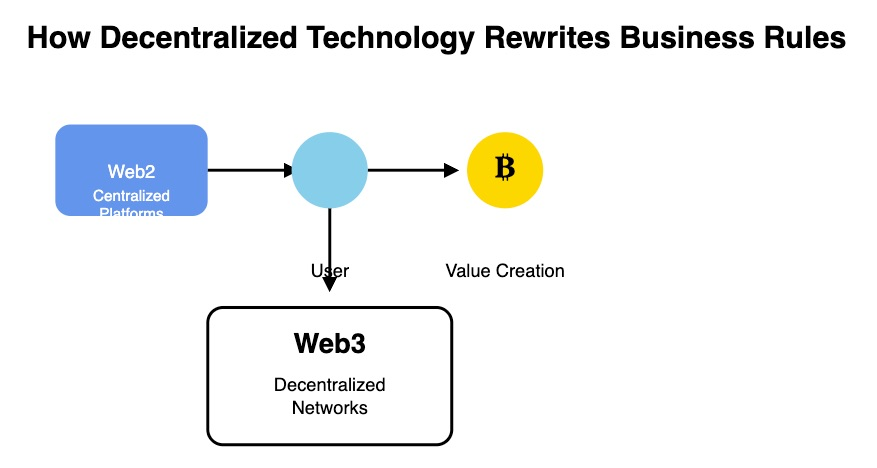
\includegraphics[keepaspectratio]{_resources/assets/images/ch2-overview.jpg}}

\section{Data Sovereignty Revolution}\label{data-sovereignty-revolution}

Web3 technologies introduce the possibility of data sovereignty,
fundamentally altering the balance of power between platforms and users.
In current systems, every click, purchase, search, and interaction
generates data that flows to platform owners who use this information to
optimize their own revenue generation. Users have no visibility into how
their data is collected, processed, or monetized, and receive no
compensation for the value their activities create.

Decentralized identity systems enable individuals to own and control
their digital identities across multiple platforms and applications.
Rather than creating separate accounts for each service and surrendering
personal information to each platform, users can maintain portable
identities that they fully control. This shift has profound implications
for how digital commerce functions, as it eliminates platforms' ability
to trap users through data lock-in effects.

When users own their data, they can choose which information to share
with different services and under what conditions. They can grant
temporary access permissions that can be revoked at any time. Most
importantly, they can negotiate compensation for sharing valuable data
or participating in data-generating activities. This creates market
mechanisms for data exchange rather than the current system of
uncompensated extraction.

The implications extend to customer relationships in commercial
contexts. Merchants who interact with customers through Web3 systems can
develop direct relationships without intermediary platforms controlling
access. Customer data remains with customers, who can choose to share
purchase history, preferences, and other valuable information directly
with merchants they trust. This enables more genuine relationships
between businesses and customers while eliminating the platform tax on
these interactions.

Decentralized storage systems ensure that user data cannot be lost,
corrupted, or manipulated by platform owners. Information stored on
distributed networks remains accessible to users regardless of what
happens to any particular platform or service provider. This creates
genuine data portability, enabling users to move between services while
maintaining their digital history and relationships.

The data sovereignty revolution also enables new forms of value creation
through user participation. When users own their data and interactions,
they can choose to monetize these assets directly rather than allowing
platforms to capture all the value. This might involve selling data to
researchers, participating in content creation that generates direct
revenue, or contributing to network effects that create tokenized
rewards.

\section{From Consumer to
Stakeholder}\label{from-consumer-to-stakeholder}

Traditional platform relationships cast users as consumers who purchase
products or services in exchange for money, or as content creators who
provide material in exchange for platform-mediated revenue sharing. Web3
systems enable a fundamental role transformation where users become
stakeholders with ownership interests in the platforms and networks they
help create and maintain.

This transformation occurs through token-based ownership systems that
distribute economic rights to network participants based on their
contributions to network value. Rather than working for platforms that
capture most of the value from user activities, participants can earn
ownership stakes in the networks they help build and maintain. These
ownership stakes typically take the form of governance tokens that
provide voting rights on network decisions and economic tokens that
entitle holders to shares of network revenue.

The stakeholder model aligns incentives between platforms and
participants in ways that platform-based systems cannot achieve. When
users own portions of the networks they participate in, they benefit
directly from network growth and success. This creates powerful
incentives for users to contribute high-quality content, provide helpful
feedback, recruit new participants, and support network development in
other ways. The result is typically faster growth and higher-quality
outcomes than centralized platforms can achieve through purely
extractive relationships.

Governance rights associated with stakeholder positions enable genuine
democratic participation in platform development and policy decisions.
Rather than accepting whatever changes platform owners decide to
implement, stakeholders can propose modifications, vote on important
decisions, and collectively guide network evolution. This creates
systems that remain responsive to participant needs rather than
optimizing solely for owner benefit.

The economic implications of stakeholder participation compound over
time as successful networks grow in value. Early participants who help
establish and develop networks can see substantial appreciation in their
ownership stakes as networks achieve scale and adoption. This creates
incentives for long-term commitment and high-quality participation
rather than the short-term extraction that characterizes many platform
relationships.

Furthermore, stakeholder models enable risk sharing and collaborative
investment in network development. When participants have ownership
stakes, they become willing to invest time, money, and effort in network
improvements because they will share in the benefits of these
investments. This can accelerate innovation and development compared to
systems where only platform owners benefit from network improvements.

\section{Smart Contract Commerce}\label{smart-contract-commerce}

Smart contracts represent one of the most significant innovations in
Web3 technology, enabling automated execution of agreements without
requiring trusted intermediaries. In commercial contexts, smart
contracts can automate payment processing, enforce service agreements,
distribute revenue shares, and manage complex multi-party transactions
with mathematical precision and complete transparency.

The elimination of intermediaries through smart contract automation
reduces transaction costs while increasing reliability and speed of
execution. Traditional commercial transactions often require banks,
payment processors, escrow services, and other intermediaries to ensure
that all parties fulfill their obligations. Each intermediary adds cost,
complexity, and potential points of failure to the transaction process.
Smart contracts can replace many of these intermediaries with automated
code that executes predefined logic when specified conditions are met.

Consider a typical e-commerce transaction involving a merchant,
customer, payment processor, and shipping company. Traditional systems
require multiple intermediaries to coordinate these interactions, with
each taking fees and introducing delays. A smart contract system could
automatically process payment when goods are delivered, distribute
appropriate portions to the merchant and shipping company, handle tax
calculations, and trigger customer service processes if problems arise.
The entire transaction executes according to predefined rules without
requiring manual intervention or intermediary coordination.

Smart contracts also enable more sophisticated commercial arrangements
that would be impractical to manage through traditional systems. Revenue
sharing agreements between multiple parties can be automated to ensure
accurate and timely distribution of funds according to complex formulas.
Subscription services can automatically adjust pricing based on usage
patterns or market conditions. Insurance claims can be processed
automatically when triggering events occur. These capabilities enable
new business models that were previously too complex or expensive to
implement.

The transparency of smart contract systems builds trust between
commercial partners by making all transaction logic visible and
verifiable. Participants can examine the code that governs their
interactions, ensuring that automated systems will behave as expected.
This transparency reduces disputes and enables cooperation between
parties who might not otherwise trust each other to honor complex
agreements.

Smart contracts also enable programmable money that can automatically
enforce spending rules, savings goals, and investment strategies. Rather
than relying on individual discipline or third-party financial services,
individuals can create automated systems that allocate income according
to predetermined rules, invest in diversified portfolios, and execute
complex financial strategies without ongoing manual management.

\section{The Death of Middlemen}\label{the-death-of-middlemen}

Web3 technologies enable direct peer-to-peer transactions that eliminate
many traditional intermediary roles while creating new forms of value
creation through network participation. Rather than paying
intermediaries to facilitate transactions, participants can interact
directly while contributing to shared infrastructure that serves their
collective interests.

Decentralized finance protocols demonstrate how intermediary elimination
works in practice. Traditional banking requires customers to deposit
money with financial institutions that then lend these funds to
borrowers while capturing the interest rate spread. DeFi protocols
enable depositors to lend directly to borrowers through automated
systems, often earning higher returns while borrowers pay lower rates.
The intermediary profits are eliminated, with the savings shared between
lenders and borrowers.

Similar dynamics apply to many other commercial sectors. Content
creators can distribute their work directly to audiences through
decentralized platforms, keeping larger portions of revenue that would
otherwise flow to platform intermediaries. Freelancers can connect with
clients through peer-to-peer networks that charge minimal fees compared
to traditional freelancing platforms. Merchants can sell directly to
consumers through decentralized marketplaces that take smaller
commissions than centralized platforms.

The elimination of intermediaries does not mean the elimination of
valuable services that intermediaries traditionally provided. Instead,
these services become distributed among network participants or
automated through smart contracts. Quality assurance, dispute
resolution, payment processing, and other intermediary functions
continue to exist but are provided through decentralized mechanisms
rather than centralized intermediaries.

This transition creates opportunities for individuals to earn income by
providing specific services within decentralized networks rather than
working for intermediary companies. Network participants can earn
rewards for content moderation, dispute resolution, quality
verification, customer service, and many other functions that were
previously performed by platform employees. This creates more flexible
and often more lucrative opportunities for individuals while reducing
the overhead costs associated with centralized intermediary
organizations.

The death of traditional intermediaries also enables more direct
relationships between producers and consumers, leading to better price
discovery and more efficient markets. When multiple layers of
intermediaries are removed, both producers and consumers can capture
larger portions of the value created through their interactions. This
typically results in lower prices for consumers and higher revenues for
producers, with the difference representing the elimination of
intermediary extraction.

\section{Implications for Business
Strategy}\label{implications-for-business-strategy}

The transition to Web3 commerce requires fundamental changes in how
businesses approach customer acquisition, relationship management, and
value creation. Companies that understand and adapt to these changes
will find significant competitive advantages, while those that cling to
platform-dependent strategies may find themselves increasingly
disadvantaged.

Customer acquisition in Web3 environments focuses on providing genuine
value and building trust rather than purchasing attention through
advertising platforms. Since Web3 users own their data and identities,
they can more easily evaluate and compare different options. Businesses
must compete on the basis of actual value provided rather than marketing
sophistication or advertising spending power.

Relationship management shifts from platform-mediated interactions
toward direct engagement with customers who own their data and
identities. This enables deeper, more authentic relationships but
requires businesses to provide ongoing value rather than relying on
platform lock-in effects to maintain customer loyalty. Companies that
excel at creating genuine value for customers will thrive, while those
that depend on information asymmetries or switching costs will struggle.

Value creation opportunities expand significantly in Web3 environments
as businesses can participate in network effects and token economies
rather than simply extracting profits from transactions. Companies can
create and participate in decentralized networks that grow in value as
they attract more participants. This can provide exponential growth
opportunities that are not available through traditional business
models.

The Web3 transition represents both a technological shift and a
philosophical evolution toward more equitable and efficient forms of
digital commerce. As we will explore in Chapter 3, the practical
implementation of these principles requires systematic approaches to
platform design, token economics, and community governance. The six
pillars of OnChain Commerce provide a framework for understanding how
these abstract concepts translate into concrete business systems that
can operate at scale while maintaining the benefits of decentralization
and participant ownership.

\chapter{The Six Pillars of OnChain Commerce}\label{sec-six-pillars}

The architectural foundation of decentralized business

The transformation from traditional platform-based commerce to
decentralized OnChain Commerce requires more than technological
innovation alone. It demands a comprehensive framework that addresses
the fundamental challenges of trust, value distribution, scalability,
and sustainable growth that have constrained previous attempts at
creating equitable digital economies. The six pillars of OnChain
Commerce provide this framework, offering a systematic approach to
building commercial systems that can operate at scale while maintaining
the benefits of decentralization and participant ownership.

These pillars work together as an integrated system rather than
independent components. Each pillar addresses specific weaknesses in
traditional commercial systems while reinforcing the others to create
stable, self-sustaining economic ecosystems. The interdependence among
the pillars ensures that OnChain Commerce systems can achieve both the
efficiency required for practical adoption and the fairness necessary
for long-term participant commitment.

Understanding these pillars requires examining both their individual
functions and their collective operation within complete OnChain
Commerce implementations. As we explored in Chapters 1 and 2, the shift
toward circulation-based wealth creation and Web3's disruption of
traditional platform models creates opportunities for new approaches to
commercial organization. The six pillars provide the specific mechanisms
through which these opportunities can be realized in practice.

\begin{figure}[H]

{\centering \pandocbounded{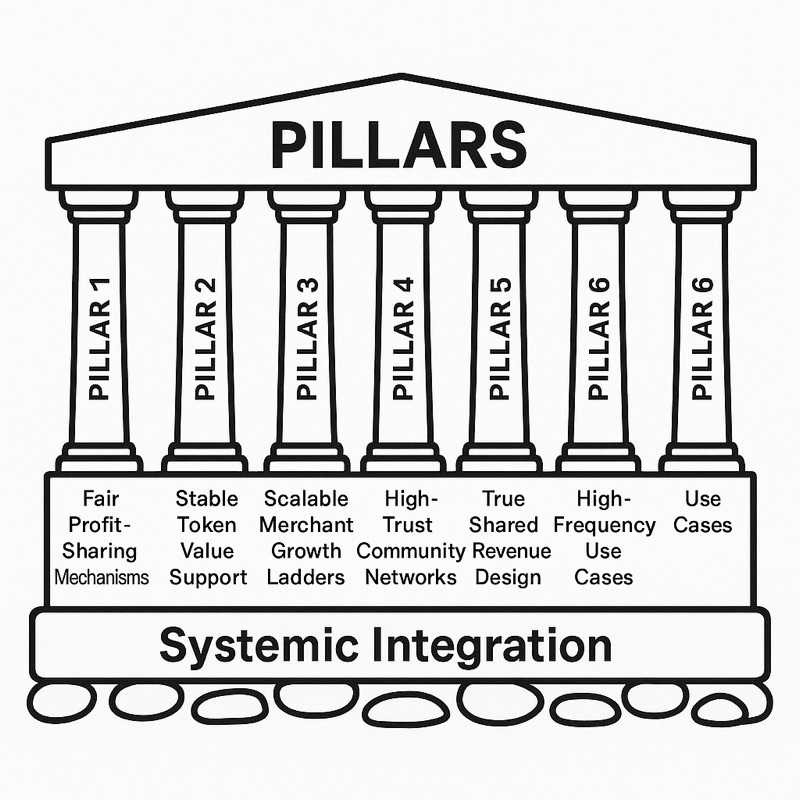
\includegraphics[keepaspectratio]{_resources/assets/images/Ch3-6-pillars.jpg}}

}

\caption{The Six Pillars}

\end{figure}%

\section{Pillar 1: Fair Profit-Sharing
Mechanisms}\label{pillar-1-fair-profit-sharing-mechanisms}

Traditional commercial systems concentrate profits among platform owners
and investors while distributing only wages or small commissions to the
participants who actually create value through their activities. OnChain
Commerce systems reverse this dynamic by implementing automatic
profit-sharing mechanisms that distribute value among all contributors
based on their actual contributions to network success.

Fair profit-sharing operates through smart contracts that automatically
allocate portions of transaction revenue among different participants
according to predefined formulas. When a customer makes a purchase
through an OnChain Commerce system, the transaction value flows through
automated distribution mechanisms that immediately allocate appropriate
portions to the merchant, the customer, referral partners, network
infrastructure providers, and other contributors to the transaction's
success.

The automation eliminates disputes and delays that characterize
traditional profit-sharing arrangements. Participants receive their
allocated portions immediately upon transaction completion, with all
calculations performed transparently according to publicly auditable
smart contract code. This creates trust through mathematical certainty
rather than relying on institutional promises or legal enforcement
mechanisms.

The specific allocation formulas can be customized for different types
of businesses and markets while maintaining core principles of fairness
and transparency. A typical distribution might allocate sixty percent of
transaction value to the customer as rewards, fifteen percent to the
merchant as incentive compensation, four percent to referral partners,
three percent to regional coordinators, and eighteen percent distributed
among various network participants according to their contributions to
the transaction's facilitation.

These percentages represent more than simple revenue sharing. They
constitute a fundamental restructuring of how commercial value is
created and distributed. Rather than extracting value from participants
to maximize platform profits, OnChain Commerce systems optimize for
participant success and network growth. This creates positive feedback
loops where successful participants attract more activity to the
network, generating increased value for all participants.

The profit-sharing mechanisms also extend beyond individual transactions
to encompass network growth and development. Participants who contribute
to network expansion, quality improvement, or infrastructure development
receive ongoing compensation from the increased value their
contributions create. This aligns individual incentives with collective
network success in ways that traditional employment or contractor
relationships cannot achieve.

Furthermore, the transparent nature of automated profit-sharing enables
participants to understand exactly how their compensation is calculated
and to verify that they receive fair treatment. This transparency
reduces conflicts and builds trust among participants who might
otherwise be skeptical of revenue-sharing claims.

\section{Pillar 2: Stable Token Value Support (AC
Model)}\label{pillar-2-stable-token-value-support-ac-model}

Many blockchain projects have failed because their tokens lacked
meaningful value backing, leading to speculation, volatility, and
eventual collapse when speculative interest waned. The Apollo Coin (AC)
model addresses this fundamental weakness by creating stable value
support through real economic activity rather than speculative trading.

The AC model links token creation directly to actual commercial
transactions rather than arbitrary token generation. When merchants
participate in OnChain Commerce systems by offering percentage discounts
on their products, these discount amounts are converted into AC tokens
that are distributed to customers and other network participants. This
ensures that every AC token represents real economic value that was
actually generated through productive commercial activity.

The mathematical foundation of AC value support operates through a
reserve fund mechanism. When customers make purchases and receive AC
tokens equivalent to merchant discounts, the corresponding dollar
amounts are deposited into decentralized reserve funds that provide
backing for AC token value. This creates a direct relationship between
AC tokens in circulation and actual dollars held in reserve, similar to
how traditional currency systems operated under gold standard
mechanisms.

Market dynamics further stabilize AC value through natural supply and
demand balancing. When AC tokens trade below their reserve-backed value,
arbitrage opportunities emerge for purchasing undervalued tokens and
redeeming them for their underlying reserve value. Conversely, when
tokens trade above reserve value, additional tokens can be created
through new commercial transactions, increasing supply until prices
stabilize near intrinsic value levels.

The stability mechanisms enable AC tokens to function as practical
currency for daily transactions rather than speculative investment
vehicles. Merchants can accept AC payments with confidence that token
values will remain relatively stable. Customers can hold AC tokens
without fear of sudden value collapses that characterize many
cryptocurrency projects. This stability is essential for building trust
and enabling widespread adoption among participants who need reliable
value storage and exchange mechanisms.

The AC model also creates built-in incentives for network growth and
adoption. As more merchants join the system and offer discounts that
convert to AC tokens, the total reserve backing increases, providing
stronger support for token values. Simultaneously, increased merchant
participation creates more opportunities for AC token usage, increasing
demand for tokens and supporting price stability through fundamental
supply and demand dynamics.

The reserve backing system is transparent and auditable, enabling
participants to verify that sufficient reserves exist to support
outstanding token values. This transparency builds confidence in the
system and reduces the risk of speculative bubbles or value collapses
that have plagued other token-based projects.

\section{Pillar 3: Scalable Merchant Growth
Ladders}\label{pillar-3-scalable-merchant-growth-ladders}

OnChain Commerce systems must accommodate participants ranging from
individual entrepreneurs to large established businesses while providing
pathways for growth and development that benefit both individual
merchants and the broader network. The scalable merchant growth ladder
creates structured progression opportunities that encourage
participation and investment while maintaining network cohesion and
shared values.

The foundation level welcomes individual entrepreneurs and small
businesses with minimal barriers to entry. New merchants can join
OnChain Commerce networks without significant upfront investments or
complex qualification processes. They gain immediate access to
token-based reward systems, automated payment processing, and basic
marketing tools that help them establish their businesses within the
network ecosystem.

As merchants achieve specific milestones related to transaction volume,
customer satisfaction, and network contribution, they unlock access to
enhanced features and benefits. The growth ladder might include access
to advanced analytics tools, priority customer service, expanded token
allocation percentages, and collaboration opportunities with other
successful merchants within the network.

Regional partnership opportunities represent the next level of merchant
development, enabling successful individual merchants to coordinate with
others in their geographic areas to create local business ecosystems.
Regional partners can pool resources for marketing campaigns, share
customer bases, and develop complementary service offerings that
increase value for local customers while strengthening the overall
network presence in their markets.

The highest levels of merchant participation involve strategic
partnerships with the core network development team, enabling large
merchants to influence network direction and development priorities
while taking on greater responsibilities for network growth and
stability. These strategic partners might operate multiple locations,
mentor new merchants, or provide specialized services that benefit the
entire network ecosystem.

The ladder structure creates clear incentives for long-term
participation and investment in network success. Merchants understand
that their growth within the network depends on providing genuine value
to customers and contributing positively to network development. This
aligns individual success with collective network prosperity in ways
that traditional business development programs often fail to achieve.

Each level of the growth ladder provides meaningful benefits that
justify the increased commitments and responsibilities associated with
advancement. The progression from individual entrepreneur to regional
partner to strategic alliance creates a career development path that can
accommodate lifelong business growth while maintaining connection to the
OnChain Commerce network.

The scalable structure also ensures that network governance remains
responsive to participant needs across different business sizes and
development stages. Individual entrepreneurs have voice in network
decisions through democratic governance mechanisms, while larger
strategic partners provide stability and resources for network
development and expansion.

\section{Pillar 4: High-Trust Community
Networks}\label{pillar-4-high-trust-community-networks}

Traditional multi-level marketing and pyramid schemes create superficial
community structures that ultimately prioritize recruitment and
hierarchy over genuine value creation and mutual support. OnChain
Commerce networks build authentic community relationships based on
shared success, transparent operations, and collaborative value creation
rather than extraction and exploitation.

The foundation of high-trust community networks lies in eliminating the
structural incentives that create exploitation in traditional systems.
OnChain Commerce participants do not profit primarily from recruiting
new members or building downline organizations. Instead, their success
depends on facilitating genuine value creation through merchant
services, customer satisfaction, and network development activities that
benefit all participants.

Network transparency creates accountability mechanisms that prevent the
development of exploitative relationships. All transactions, reward
distributions, and governance decisions are recorded on blockchain
systems that enable any participant to verify fair treatment and
appropriate compensation. This transparency eliminates the information
asymmetries that enable manipulation and exploitation in traditional
hierarchical systems.

The community network structure emphasizes horizontal collaboration
rather than vertical hierarchy. Participants at similar levels of
network involvement work together to solve problems, share resources,
and develop new opportunities rather than competing against each other
for limited positions in organizational hierarchies. This collaborative
approach creates stronger relationships and more sustainable community
bonds.

Regional clustering enables local community development while
maintaining connection to the broader global network. Participants in
specific geographic areas can develop personal relationships, coordinate
local marketing efforts, and provide mutual support while benefiting
from the resources and opportunities available through the larger
network. This balance between local community and global network access
provides both personal connection and scalable opportunity.

Educational and support systems ensure that all community members have
access to the knowledge and resources necessary for success within the
network. Rather than hoarding information to maintain competitive
advantages, successful participants are incentivized to share knowledge
and provide mentorship because network growth benefits everyone through
increased activity and token value appreciation.

Conflict resolution mechanisms enable community members to address
disputes and disagreements through transparent, fair processes rather
than relying on arbitrary decisions by authority figures. Decentralized
governance systems provide structured approaches to problem-solving that
maintain community cohesion while protecting individual rights and
interests.

The high-trust community networks also create social validation and
support systems that help participants maintain motivation and
commitment during challenging periods. The combination of financial
incentives and social relationships creates stronger participant
retention than purely economic arrangements can achieve.

\section{Pillar 5: True Shared Revenue
Design}\label{pillar-5-true-shared-revenue-design}

Most traditional revenue-sharing programs provide token amounts or
conditional benefits that do not represent genuine profit participation.
OnChain Commerce systems implement true shared revenue designs where
participants receive meaningful portions of actual network profits
rather than nominal rewards or limited discount programs.

True shared revenue operates through mathematical formulas that allocate
specific percentages of network revenue among different categories of
participants based on their contributions to network success. These
allocations represent real economic value rather than promotional
gimmicks or marketing expenses. Participants understand that their
compensation comes from genuine profit-sharing rather than new
participant recruitment or other unsustainable sources.

The revenue sharing extends beyond immediate transaction rewards to
encompass ongoing network profitability. As OnChain Commerce networks
grow and generate increased transaction volume, all participants benefit
from this growth through increased revenue sharing rather than having
growth benefits captured exclusively by platform owners or early
investors.

Network participants earn revenue sharing through multiple types of
contributions rather than single activities. Customer referrals,
merchant support, content creation, network governance participation,
and infrastructure development can all generate revenue sharing based on
their actual value contributions to network success. This diversity of
value creation opportunities ensures that participants with different
skills and interests can find meaningful ways to contribute and benefit.

The shared revenue design also includes appreciation opportunities
through token ownership. As networks grow and become more valuable,
participants who own AC tokens benefit from value appreciation in
addition to ongoing revenue sharing. This creates both immediate income
opportunities and long-term wealth building possibilities for active
network participants.

Transparency in revenue calculation and distribution ensures that
participants can verify their fair treatment and understand how their
contributions translate into compensation. Regular reporting and
auditable smart contract systems provide visibility into network
financial performance and revenue allocation, building trust and
enabling participants to make informed decisions about their level of
network involvement.

The revenue sharing formulas can evolve over time through democratic
governance processes, ensuring that compensation structures remain fair
and competitive as network conditions change. Participants have voice in
decisions about revenue allocation priorities and can propose
modifications that better serve network development and participant
interests.

\section{Pillar 6: High-Frequency Use
Cases}\label{pillar-6-high-frequency-use-cases}

Successful OnChain Commerce networks must serve real business needs with
high-frequency use cases rather than depending on speculative trading or
novel applications that lack practical utility. The sixth pillar ensures
that network activity is driven by genuine economic demand rather than
artificial adoption incentives or speculative investment.

High-frequency use cases focus on essential daily business activities
rather than occasional or luxury transactions. Food service, retail
merchandise, personal services, and professional services represent the
types of businesses that generate consistent customer demand and repeat
transactions. These sectors provide the transaction volume necessary to
support robust token economies while serving genuine market needs.

The integration of OnChain Commerce systems into existing business
operations ensures that network adoption serves practical business
improvement rather than requiring complete operational transformation.
Merchants can implement token-based reward systems alongside traditional
payment methods, gradually increasing OnChain Commerce integration as
they become comfortable with the systems and observe positive results.

Geographic concentration strategies enable OnChain Commerce networks to
achieve critical mass within specific regions before expanding to new
markets. When sufficient merchants within a local area participate in
the network, customers can use AC tokens for many of their daily
purchases, creating practical utility that supports token demand and
network growth.

Cross-merchant compatibility ensures that tokens earned from one
business can be used with other network merchants, creating utility that
exceeds what any individual merchant could provide. Customers who
receive AC tokens from restaurant purchases can use these tokens for
retail shopping, personal services, or other participating businesses,
creating network effects that benefit all merchants.

Service quality standards maintain customer satisfaction and retention
by ensuring that OnChain Commerce merchants provide positive customer
experiences. Network governance systems can implement quality monitoring
and improvement programs that protect network reputation and encourage
continued customer participation.

The high-frequency focus also enables rapid feedback cycles that support
continuous network improvement. When systems serve daily business needs,
problems and opportunities become apparent quickly, enabling responsive
development and optimization that keeps network services aligned with
practical business requirements.

Integration with existing payment and business management systems
reduces barriers to merchant adoption while providing seamless customer
experiences. OnChain Commerce systems that work alongside familiar
business tools and processes achieve faster adoption than those
requiring complete operational transformation.

\section{Systemic Integration and
Synergies}\label{systemic-integration-and-synergies}

The six pillars function as an integrated system where each pillar
reinforces and amplifies the others to create stable, growing OnChain
Commerce networks. Fair profit-sharing creates incentives for
participation, while stable token value support enables practical usage.
Merchant growth ladders provide development pathways that high-trust
communities support through collaboration and knowledge sharing. True
shared revenue design rewards genuine contributions, while
high-frequency use cases provide the transaction volume necessary to
sustain revenue generation.

This systemic integration creates positive feedback loops that
strengthen network effects over time. As more merchants join and offer
high-frequency services, token utility increases, supporting token
values and enabling more generous profit-sharing. Improved
profit-sharing attracts more participants, expanding the community
networks that support merchant growth and service quality. The resulting
growth creates more revenue for true sharing among participants,
creating sustainable cycles of expansion and value creation.

The interdependence among pillars also provides stability against
external challenges and market fluctuations. Networks that depend on
single benefits or isolated features can collapse when those specific
advantages disappear. OnChain Commerce networks built on all six pillars
maintain multiple sources of value and resilience that enable adaptation
to changing conditions while preserving core participant benefits.

As we will explore in Chapter 4, these architectural foundations enable
the specific mechanisms through which spending can become investment and
consumption can generate wealth for participants. The six pillars
provide the infrastructure necessary to implement the ``spend more, earn
more'' operating system that distinguishes OnChain Commerce from
traditional business models.

\part{Part II: The Mechanics of Transformation}

\chapter{The ``Spend More, Earn More'' Operating
System}\label{sec-spend-earn-system}

How consumption becomes investment in the new economy

The concept that spending money can actually increase wealth rather than
diminish it represents one of the most counterintuitive aspects of
OnChain Commerce systems. Traditional economic thinking treats
consumption and investment as opposing activities: money spent on goods
and services is no longer available for wealth-building investments.
OnChain Commerce fundamentally restructures this relationship by
creating mechanisms through which consumption activities simultaneously
generate investment returns for participants.

This transformation occurs through sophisticated token distribution
systems that convert portions of consumer spending into tradeable
digital assets while maintaining the fundamental value exchange that
characterizes normal commercial transactions. Customers receive the
goods and services they purchase while also receiving tokens that
represent ownership stakes in the commercial network that facilitated
their purchases. The result is a system where increased participation
and spending generates increased wealth accumulation rather than
depleting financial resources.

Understanding how this system operates requires examining the specific
mechanisms through which traditional consumption expenditures are
converted into investment assets, the mathematical foundations that
ensure sustainable returns, and the economic principles that enable such
systems to create genuine value rather than simply redistributing
existing wealth among participants.

\section{Transaction-to-Asset
Conversion}\label{transaction-to-asset-conversion}

The foundational mechanism of spend-more-earn-more systems lies in the
automatic conversion of transaction amounts into token assets that
appreciate over time. When a customer makes a purchase through an
OnChain Commerce platform, the merchant's profit-sharing commitment is
immediately converted into Apollo Coin (AC) tokens that are distributed
to the customer and other network participants according to
predetermined allocation formulas.

This conversion process operates through smart contracts that
automatically execute complex calculations and distributions without
requiring manual intervention or trust in third-party administrators.
The merchant sets a profit-sharing percentage that represents the
portion of gross sales they are willing to allocate toward network token
distribution. This percentage, typically ranging from three to
ninety-nine percent of transaction value, represents real economic value
that the merchant forgoes in exchange for the marketing benefits and
customer loyalty generated by participating in the OnChain Commerce
network.

Consider a specific example of how this conversion operates in practice.
A customer purchases a fifty-dollar meal at a restaurant that
participates in OnChain Commerce with a thirty percent profit-sharing
commitment. The customer pays fifty dollars and receives their meal,
exactly as in any traditional transaction. Additionally, however, the
smart contract system automatically converts fifteen dollars (thirty
percent of fifty dollars) into AC tokens based on current market
exchange rates and distributes these tokens according to the network's
allocation formula.

Using the distribution model discussed in Chapter 3, sixty percent of
the converted amount would flow to the customer as rewards, fifteen
percent to the merchant as participation incentives, four percent to
referral partners, three percent to regional coordinators, and the
remaining eighteen percent distributed among various network
infrastructure participants. This means the customer would receive AC
tokens worth nine dollars, while the merchant receives tokens worth two
dollars and twenty-five cents, despite having contributed fifteen
dollars worth of profit margin to the conversion pool.

The transaction-to-asset conversion creates immediate value for
customers while establishing long-term relationships that benefit
merchants through increased customer loyalty and repeat business.
Customers develop financial incentives to return to participating
merchants because their spending generates ongoing investment returns
through token appreciation. Merchants benefit from reduced customer
acquisition costs and increased transaction frequency, often more than
compensating for the profit margins allocated to token distribution.

The conversion mechanism also creates network effects that benefit all
participants as the system grows. Each transaction strengthens the
reserve backing for AC tokens while demonstrating real economic demand
for network services. This combination of reserve strengthening and
demand validation supports token value appreciation that benefits all
token holders throughout the network.

Furthermore, the automatic nature of transaction-to-asset conversion
eliminates the complexity and barriers that often prevent consumer
participation in traditional investment programs. Customers do not need
to understand token mechanics, manage digital wallets, or make explicit
investment decisions. The conversion occurs seamlessly as part of normal
shopping activities, making investment participation accessible to
individuals who might never engage with traditional cryptocurrency or
investment systems.

\section{The AC Token Economy}\label{the-ac-token-economy}

The Apollo Coin token economy provides the mathematical foundation that
enables sustainable spend-more-earn-more operations. Unlike speculative
cryptocurrencies that derive value primarily from trading activity and
market sentiment, AC tokens are backed by real economic reserves
generated through actual commercial transactions. This backing creates
intrinsic value that supports long-term price stability and appreciation
based on fundamental economic activity rather than speculative bubbles.

The reserve backing system operates through decentralized smart
contracts that automatically deposit portions of merchant profit-sharing
contributions into reserve pools. These reserves are held in stable
cryptocurrencies such as USDC (US Dollar Coin) that maintain reliable
value relationships with traditional currencies. The reserve pools
provide mathematical support for AC token values while enabling token
holders to redeem tokens for underlying reserve assets under specific
conditions.

The relationship between circulating AC tokens and reserve backing
creates natural price stabilization mechanisms. When AC tokens trade
below their reserve-backed intrinsic value, arbitrage opportunities
emerge for purchasing undervalued tokens and potentially redeeming them
for higher-value reserve assets. Conversely, when tokens trade above
intrinsic value, additional token creation through new merchant
transactions increases supply until prices stabilize near mathematically
supported levels.

The token economy also incorporates velocity incentives that encourage
circulation rather than hoarding. AC tokens generate additional value
when used for purchases within the network rather than held as static
investments. Network participants who actively spend AC tokens with
participating merchants often receive bonus allocations, referral
rewards, or other incentives that increase their total token
accumulation compared to passive holders.

The mathematical models underlying AC token distribution ensure that
network growth creates positive-sum outcomes rather than zero-sum
redistribution. As more merchants join the network and contribute
profit-sharing to the reserve pools, the total backing for all
outstanding tokens increases. Simultaneously, increased merchant
participation creates more opportunities for token utilization,
generating demand that supports price appreciation through fundamental
supply and demand dynamics.

Geographic expansion strategies further strengthen the token economy by
creating multiple regional markets that support token utility and
demand. When sufficient merchants within specific geographic areas
participate in the network, customers can use AC tokens for many of
their daily purchases, creating practical utility that transcends
speculative trading value. This utility-based demand provides
sustainable support for token values independent of cryptocurrency
market fluctuations.

The transparency of reserve backing and token distribution creates
accountability that builds participant confidence in the system's
long-term sustainability. Unlike traditional investment programs that
rely on institutional promises or complex financial engineering, AC
token holders can verify the mathematical relationships between their
token holdings and underlying reserve assets through blockchain-based
auditing systems.

\section{Closed-Loop Value Systems}\label{closed-loop-value-systems}

The most sophisticated aspect of spend-more-earn-more systems lies in
their creation of closed-loop value systems that amplify benefits for
participants while reducing dependency on external economic conditions.
These systems achieve sustainability by creating multiple interconnected
value streams that reinforce each other through network effects and
participant behavior optimization.

The primary loop operates through customer spending, token accumulation,
and reinvestment within the network. Customers who receive AC tokens
through their purchases are incentivized to spend these tokens with
other network merchants, both to utilize their token value and to
generate additional token rewards through continued network
participation. This creates a circulation pattern where tokens flow
between customers and merchants while generating incremental value at
each transaction point.

Secondary loops emerge through referral and community building
activities that expand network participation and increase total
transaction volume. Participants who successfully recruit new merchants
or customers to the network receive ongoing compensation from the
increased activity their referrals generate. This creates incentives for
network evangelism and growth that benefit existing participants through
increased token utility and appreciation rather than simply diluting
existing value among more participants.

The merchant ecosystem creates additional value loops through
collaboration and cross-referral activities. Participating merchants
often develop complementary relationships where they refer customers to
each other for services outside their own specialties. A restaurant
might partner with a nearby spa, retail store, or entertainment venue to
create comprehensive local networks that increase customer convenience
while generating referral income for participating businesses.

Regional coordination mechanisms enable local merchant networks to pool
resources for marketing campaigns, customer acquisition programs, and
infrastructure development that benefits all network participants. These
collaborative investments generate returns that are distributed among
participating merchants according to their contribution levels and
network activity, creating incentives for collective rather than purely
individual optimization.

The closed-loop systems also incorporate feedback mechanisms that
optimize network performance based on participant behavior and outcomes.
Analytics systems track customer satisfaction, merchant profitability,
token circulation patterns, and network growth metrics to identify
optimization opportunities and adjust system parameters for improved
performance. This continuous improvement process ensures that the
networks evolve to better serve participant needs while maintaining
mathematical sustainability.

Quality assurance loops maintain network integrity by monitoring
merchant performance and customer satisfaction levels. Merchants who
consistently provide positive customer experiences receive enhanced
benefits and promotional support, while those who generate complaints or
negative feedback may face reduced participation benefits or removal
from the network. This creates incentives for service quality that
protect network reputation and customer retention.

The integration of multiple value loops creates resilience against
external economic disruptions. When traditional economic conditions
deteriorate, closed-loop networks can continue generating value for
participants through internal circulation and exchange activities. This
resilience becomes particularly valuable during economic uncertainty
when traditional investment and employment opportunities may become less
reliable.

\section{Risk Mitigation and System
Safeguards}\label{risk-mitigation-and-system-safeguards}

The spend-more-earn-more model incorporates comprehensive risk
mitigation strategies that distinguish it from gambling, speculation, or
unsustainable financial schemes. These safeguards protect participant
investments while ensuring system sustainability through conservative
mathematical models and transparent operational procedures.

Reserve backing requirements ensure that token values are supported by
real economic assets rather than speculative market sentiment. The
percentage of reserve backing relative to outstanding tokens is
maintained through algorithmic controls that prevent over-issuance of
tokens relative to available reserve funds. This creates mathematical
floors for token values that protect participants against total loss
scenarios that characterize purely speculative investments.

Merchant vetting procedures verify the legitimacy and sustainability of
businesses before they can participate in profit-sharing programs. New
merchants must demonstrate stable business operations, appropriate
licensing and registration, and sufficient transaction volume to support
their proposed profit-sharing commitments. This screening process
reduces the risk of fraudulent or unsustainable merchant participation
that could damage network integrity.

Transaction limits prevent individual participants from risking
excessive amounts relative to their financial capacity. Daily, weekly,
and monthly limits on token acquisition through spending activities
ensure that participants cannot inadvertently over-invest in network
tokens relative to their overall financial situations. These limits can
be adjusted based on participant income verification and demonstrated
understanding of system operations.

Geographic diversification spreads network risk across multiple regional
markets and economic conditions. Rather than concentrating all activity
in single locations or industries, OnChain Commerce networks
deliberately cultivate merchant diversity across geographic regions and
business sectors. This diversification reduces the impact of local
economic disruptions on overall network stability and participant
returns.

Governance mechanisms enable participant input into system modifications
and risk management policies. Token holders can propose and vote on
changes to reserve requirements, distribution formulas, merchant
qualification criteria, and other system parameters that affect network
operations and participant safety. This democratic governance ensures
that risk management policies reflect participant preferences and
evolving market conditions.

Regulatory compliance procedures ensure that network operations conform
to applicable financial regulations and consumer protection laws. Legal
frameworks governing securities, payment processing, consumer
protection, and taxation are carefully analyzed and incorporated into
system design to prevent regulatory conflicts that could threaten
network operations or participant interests.

Exit mechanisms enable participants to recover their investments under
various circumstances. Token redemption options, merchant withdrawal
procedures, and customer refund policies provide multiple pathways for
participants to exit the network if their circumstances or preferences
change. These exit options reduce participant risk while maintaining
network integrity through orderly departure procedures.

\section{Return on Investment
Analysis}\label{return-on-investment-analysis}

The mathematical foundations of spend-more-earn-more systems enable
quantitative analysis of participant returns under various scenarios and
market conditions. These calculations demonstrate how ordinary spending
activities can generate investment-like returns while maintaining the
practical utility of normal commercial transactions.

The immediate return component derives from token allocation percentages
that provide instant value back to customers from their purchases. A
customer purchasing one hundred dollars worth of goods from a merchant
with thirty percent profit-sharing would immediately receive AC tokens
worth eighteen dollars (sixty percent of the thirty-dollar conversion
amount). This represents an immediate eighteen percent return on
spending, comparable to high-yield investment returns but achieved
through normal consumption activities.

The appreciation component depends on network growth and token value
increases over time. Historical analysis of successful OnChain Commerce
implementations demonstrates annual token appreciation rates ranging
from twenty to three hundred percent, depending on network adoption
rates and regional economic conditions. Conservative projections based
on sustainable growth models suggest that token values might appreciate
fifty to one hundred percent annually under favorable but realistic
conditions.

The compound growth component emerges from reinvesting tokens within the
network to generate additional token accumulation. Customers who use
their AC tokens for subsequent purchases continue earning additional
tokens while benefiting from any appreciation in their existing token
holdings. This compounding effect can significantly amplify total
returns over time, particularly for participants who maintain high
levels of network engagement.

Regional network effects create additional return opportunities through
cross-merchant utilization and referral programs. Participants in mature
regional networks often report total annual returns exceeding two
hundred percent of their spending activities when combining immediate
token allocations, appreciation gains, referral income, and network
participation rewards. These returns reflect the network effects that
emerge when sufficient merchants and customers participate in localized
OnChain Commerce ecosystems.

Risk-adjusted return calculations account for potential token value
fluctuations and network adoption uncertainties. Even under conservative
scenarios that assume modest network growth and limited token
appreciation, participants typically achieve positive returns that
exceed traditional savings accounts, money market funds, and many
conventional investment options. The combination of immediate token
allocations and modest appreciation often generates returns that justify
participation from purely financial perspectives.

The practical benefits of increased purchasing power further enhance
effective returns through improved access to goods and services within
network merchant communities. Participants often discover new
businesses, receive preferential treatment from network merchants, and
gain access to exclusive offers and services that provide value beyond
pure financial returns. These qualitative benefits complement
quantitative returns to create comprehensive value propositions that
justify network participation.

Long-term wealth building potential emerges from sustained participation
in growing OnChain Commerce networks over multi-year periods.
Participants who maintain consistent engagement and reinvestment within
expanding networks often accumulate substantial token holdings that
appreciate significantly as networks achieve regional or national scale.
This wealth building potential transforms routine spending activities
into systematic investment programs that can generate substantial
long-term financial benefits.

The spend-more-earn-more operating system represents a fundamental
innovation in consumer economics that aligns individual spending
decisions with investment returns while supporting genuine business
development and community prosperity. As we will explore in Chapter 5,
this system operates distinctly from traditional multi-level marketing,
e-commerce, and franchising models that often create conflicts between
individual and collective interests. The mathematical foundations and
systematic safeguards of OnChain Commerce create sustainable value
generation that benefits all participants while serving real economic
needs in local and regional markets.

\chapter{Beyond MLM, E-commerce, and
Franchising}\label{sec-beyond-traditional}

Fundamental differences from traditional business models

OnChain Commerce systems are frequently misunderstood as variations of
multi-level marketing, e-commerce platforms, or franchise operations
because they share certain surface characteristics with these
traditional business models. All involve networks of participants,
revenue sharing among multiple parties, and growth through participant
recruitment and retention. However, the fundamental structures,
incentive systems, and value creation mechanisms of OnChain Commerce
differ dramatically from these traditional approaches in ways that
address the systemic problems that limit their sustainability and
fairness.

Understanding these differences requires examining not just the
operational mechanics of each model, but the underlying economic
principles and incentive structures that determine their long-term
viability and impact on participants. While traditional models often
create conflicts between individual success and collective
sustainability, OnChain Commerce aligns individual and collective
interests through carefully designed token economics and governance
mechanisms.

The distinction matters because many promising business innovations have
failed due to being built on flawed foundational assumptions borrowed
from traditional models. OnChain Commerce represents a genuinely new
approach to commercial organization that transcends the limitations of
existing frameworks while preserving their beneficial elements.

\section{The MLM Trap: Structural Flaws in Multi-Level
Marketing}\label{the-mlm-trap-structural-flaws-in-multi-level-marketing}

Multi-level marketing systems create the appearance of distributed
opportunity while actually concentrating wealth and power among early
participants at the expense of later joiners. The mathematical structure
of MLM systems ensures that the vast majority of participants will lose
money while a small percentage achieve substantial returns, creating
unsustainable dynamics that inevitably lead to system collapse.

The fundamental flaw in MLM systems lies in their dependence on
exponential recruitment growth to generate revenue for existing
participants. Each participant must recruit multiple new participants
who must each recruit additional participants to maintain income levels.
This creates pyramid structures where early participants benefit from
the efforts of increasingly large numbers of later participants without
providing proportional value in return.

Consider the mathematics of a typical MLM structure where each
participant needs to recruit five new participants to achieve meaningful
income. After five levels of recruitment, the system would require over
three thousand participants at the bottom level to support roughly six
hundred participants at higher levels. After ten levels, the bottom
level would need millions of participants, quickly exceeding the
available population in most markets. This mathematical impossibility
guarantees that most participants will fail to achieve meaningful
returns regardless of their effort or skill.

MLM systems also create perverse incentives that prioritize recruitment
over actual value creation. Participants earn more money by recruiting
new distributors than by selling products to end customers, leading to
focus on sales presentations and recruitment activities rather than
customer service and product improvement. This misalignment often
results in poor customer experiences and low-quality products that
cannot compete effectively in normal market conditions.

The inventory loading requirements common in MLM systems force
participants to purchase products they cannot sell, creating immediate
financial losses that are justified through promises of future
recruitment success. These inventory requirements generate revenue for
the MLM company while shifting financial risk to participants who must
invest their own money before earning any returns.

OnChain Commerce eliminates these structural problems by basing rewards
on actual transaction value rather than recruitment activities.
Participants earn tokens from genuine commercial transactions where
customers purchase goods and services they actually want, rather than
from selling business opportunities to new recruits. No one is required
to purchase inventory or maintain minimum purchase volumes to
participate in the system.

The token distribution mechanisms ensure that value flows to all
participants based on their contributions to network activity rather
than their position in recruitment hierarchies. Unlike MLM systems where
only top-level participants achieve substantial returns, OnChain
Commerce can provide meaningful benefits to all participants because
rewards come from shared economic value creation rather than
redistribution from lower levels to higher levels.

Furthermore, OnChain Commerce systems become more valuable as they grow,
creating positive-sum outcomes where network expansion benefits existing
participants rather than diluting their returns. MLM systems become less
sustainable as they grow because the recruitment requirements become
increasingly difficult to fulfill, while OnChain Commerce systems become
more useful and valuable as more merchants and customers participate.

\section{Platform Prison: E-commerce Dependency and
Exploitation}\label{platform-prison-e-commerce-dependency-and-exploitation}

Modern e-commerce platforms have created sophisticated systems for
extracting value from merchants while making them dependent on platform
services for market access. Amazon, eBay, Shopify, and similar platforms
initially attracted merchants by offering valuable services at
reasonable costs, but have gradually increased fees and restrictions as
merchants became dependent on platform traffic for their survival.

The platform prison operates through multiple interconnected mechanisms
that make departure increasingly costly and difficult over time.
Merchants invest substantial effort in building their platform presence,
accumulating customer reviews, optimizing for platform algorithms, and
integrating their operations with platform tools. These investments
become stranded costs if merchants attempt to leave the platform,
creating switching costs that enable platforms to gradually increase
their extraction without losing merchant participation.

Customer relationship control represents the most significant element of
platform control over merchants. Platforms own all customer data and
relationships, preventing merchants from building direct connections
with their buyers. Merchants cannot contact customers outside the
platform, cannot transfer customer lists to alternative platforms, and
cannot build brand loyalty that transcends platform dependency. This
customer relationship control ensures that merchants remain dependent on
platform services regardless of how those services evolve.

The algorithmic manipulation of merchant visibility creates artificial
scarcity that platforms monetize through advertising and premium
placement services. Merchants who previously received organic traffic
find their visibility reduced unless they purchase advertising or
premium services from the platform. This forces merchants to pay for
access to customers they previously reached through organic discovery,
gradually converting platform benefits into platform costs.

Fee escalation occurs as platforms achieve market dominance and
merchants become dependent on platform traffic. Initial fees that seemed
reasonable when platforms provided genuine value gradually increase as
platforms optimize for maximum revenue extraction. Merchants who built
their businesses around platform economics find themselves trapped
between unsustainable fee structures and the inability to replace
platform traffic through alternative channels.

OnChain Commerce addresses these problems by giving merchants direct
relationships with customers through token-based loyalty systems.
Customers who receive AC tokens from merchant purchases develop direct
financial relationships with those merchants that exist independently of
any platform intermediary. Merchants can communicate with customers,
build direct relationships, and maintain customer loyalty through token
rewards rather than depending on platform algorithms and advertising
systems.

The decentralized nature of OnChain Commerce prevents any single entity
from controlling merchant access to customers or manipulating merchant
visibility for profit. Network governance mechanisms enable merchants to
participate in decisions about network development and policy changes,
ensuring that network evolution serves merchant interests rather than
platform owner profit maximization.

Token-based customer acquisition creates sustainable customer
relationships that appreciate over time rather than becoming more
expensive. As OnChain Commerce networks grow and token values
appreciate, existing customer relationships become more valuable rather
than requiring increasing advertising spending to maintain. This creates
positive feedback loops that reward merchants for providing excellent
customer service rather than penalizing them through increased platform
fees.

\section{Franchise Limitations: Operational and
Geographic}\label{franchise-limitations-operational-and-geographic}

Traditional franchise systems offer business model replication and brand
recognition in exchange for substantial upfront investments, ongoing
royalty payments, and operational restrictions that limit franchisee
flexibility and growth potential. While franchising can provide proven
business models and marketing support, it also creates dependencies and
limitations that prevent franchisees from adapting to local market
conditions or pursuing innovative opportunities.

The franchise fee structure front-loads costs and risks onto franchisees
while ensuring revenue for franchisors regardless of franchisee success.
Initial franchise fees often range from tens of thousands to hundreds of
thousands of dollars, creating substantial financial barriers to entry
and immediate debt burdens for new franchisees. These fees must be paid
before franchisees generate any revenue from their operations, shifting
financial risk away from franchisors who have proven expertise toward
franchisees who are learning the business.

Ongoing royalty payments create permanent revenue extraction that
reduces franchisee profitability throughout the life of the franchise
relationship. Royalties typically range from four to twelve percent of
gross revenue, representing significant portions of franchisee profits
that flow to franchisors regardless of the actual support or value
provided. These ongoing payments can make the difference between
profitable and unprofitable operations for franchisees, particularly
during challenging economic periods.

Operational restrictions prevent franchisees from adapting to local
market conditions or pursuing innovative improvements to their
businesses. Franchise agreements typically specify detailed requirements
for product offerings, pricing structures, marketing approaches, vendor
relationships, and operational procedures. While this standardization
can ensure quality consistency, it also prevents franchisees from
responding to local customer preferences or competitive conditions.

Geographic exclusivity limitations restrict franchisee growth
opportunities by preventing expansion beyond designated territories.
Successful franchisees who want to open additional locations may be
restricted by geographic boundaries or required to purchase additional
franchise rights at substantial cost. These restrictions can prevent
successful franchisees from capitalizing on their expertise and market
knowledge while protecting franchisor revenue from territory sales.

Brand dependency creates vulnerabilities to franchisor decisions and
reputation management failures. Franchisees invest in building
businesses around franchisor brands, making their success dependent on
franchisor marketing effectiveness and reputation management. When
franchisors make poor decisions or face public relations problems,
franchisees suffer consequences despite having no control over the
decisions that created the problems.

OnChain Commerce provides business development benefits similar to
franchising without the restrictive contractual relationships and
ongoing fee obligations. Merchants can access proven token-based
customer loyalty systems, marketing tools, and operational best
practices through network participation without paying franchise fees or
surrendering operational control.

The open-source nature of OnChain Commerce systems enables merchants to
adapt and modify their operations based on local market conditions while
maintaining access to network benefits. Merchants can adjust their
product offerings, pricing strategies, and customer engagement
approaches to optimize for their specific markets without violating
franchise restrictions or losing network access.

Regional coordination within OnChain Commerce networks provides
collaborative marketing and development opportunities without the
hierarchical control structures that characterize franchise systems.
Merchants can work together on regional marketing campaigns, customer
acquisition programs, and business development initiatives while
maintaining their independence and operational flexibility.

The token-based reward system creates customer loyalty that benefits
individual merchants rather than franchise brands. Customers develop
financial relationships with specific merchants through token
accumulation rather than generic brand loyalty that could transfer to
any franchise location. This enables merchants to build sustainable
competitive advantages through superior customer service rather than
depending solely on brand recognition.

\section{OnChain Advantages: Improvements Over Traditional
Models}\label{onchain-advantages-improvements-over-traditional-models}

OnChain Commerce systems address the fundamental weaknesses of
traditional business models through systematic design improvements that
align individual and collective interests while preserving the
beneficial aspects of network participation and shared resources. These
improvements create sustainable competitive advantages that benefit all
participants rather than extracting value from some participants to
benefit others.

The decentralized governance structure eliminates the concentration of
power and decision-making authority that enables exploitation in
traditional systems. Rather than having centralized authorities who can
change rules, increase fees, or modify operational requirements for
their own benefit, OnChain Commerce networks operate through democratic
governance where participants vote on network modifications and policy
changes.

Transparent operations through blockchain technology ensure that all
participants can verify fair treatment and appropriate compensation.
Unlike traditional systems where fee calculations, revenue sharing, and
decision-making processes often lack transparency, OnChain Commerce
systems record all transactions and distributions on public ledgers that
anyone can audit. This transparency eliminates information asymmetries
that enable manipulation and exploitation.

The positive-sum economics of token appreciation creates value for all
participants rather than redistributing existing value from some
participants to others. As OnChain Commerce networks grow and generate
more transaction volume, token values typically appreciate, benefiting
all token holders regardless of their position in the network. This
contrasts with traditional systems where network growth often benefits
early participants at the expense of later joiners.

Direct customer relationships enable merchants to build sustainable
competitive advantages through customer service excellence rather than
depending on platform intermediaries or brand recognition. Customers who
receive tokens from merchant purchases develop direct financial
relationships that incentivize continued patronage and referrals. These
relationships belong to individual merchants rather than platforms or
franchisors.

Flexible operational structures allow merchants to adapt their
businesses to local market conditions while maintaining access to
network benefits. Unlike franchise systems that impose standardized
operational requirements, OnChain Commerce networks provide tools and
infrastructure that merchants can implement according to their specific
needs and market conditions.

Risk distribution mechanisms spread financial risks across multiple
participants and revenue streams rather than concentrating risks on
individual merchants or franchisees. Token values are supported by
reserve backing and diversified merchant networks rather than depending
on individual business success or franchisor decisions. This distributed
risk structure provides stability and resilience that benefits all
network participants.

\section{Comparative Analysis: Structural Differences and
Outcomes}\label{comparative-analysis-structural-differences-and-outcomes}

A systematic comparison of OnChain Commerce with traditional business
models reveals fundamental differences in incentive structures, risk
distribution, value creation mechanisms, and long-term sustainability
prospects. These differences explain why OnChain Commerce can achieve
outcomes that traditional models cannot sustain while avoiding the
exploitation and conflicts that ultimately undermine traditional
systems.

Revenue generation in traditional MLM systems depends on recruitment
growth that becomes mathematically impossible to sustain, while OnChain
Commerce revenue comes from genuine commercial transactions that can
grow sustainably over time. Traditional e-commerce platforms generate
revenue by extracting increasing percentages from merchant transactions,
while OnChain Commerce creates value through network effects that
benefit all participants. Franchise systems generate revenue through
upfront fees and ongoing royalties regardless of franchisee success,
while OnChain Commerce participants benefit from shared token
appreciation based on collective network success.

Risk allocation in traditional systems typically concentrates risks on
individual participants while guaranteeing returns for system operators.
MLM participants risk their investment capital and effort with no
guarantee of returns, while MLM companies receive revenue from product
sales and membership fees. E-commerce merchants risk their business
viability on platform policy changes and algorithm modifications while
platforms collect fees regardless of merchant success. Franchisees risk
substantial capital investments and ongoing royalty obligations while
franchisors receive revenue regardless of individual franchise
performance. OnChain Commerce distributes risks across diversified
merchant networks and reserve backing systems while enabling all
participants to benefit from network success.

Value creation mechanisms distinguish OnChain Commerce from traditional
models through their focus on genuine economic activity rather than
recruitment, dependency, or extraction. MLM systems primarily create
value for companies and early participants rather than for customers or
later participants. E-commerce platforms create value for platform
owners and shareholders while gradually extracting value from merchants
and customers. Franchise systems create value for franchisors and
successful franchisees while requiring substantial investments and
ongoing payments from all franchisees. OnChain Commerce creates value
for all participants through shared economic activity and token
appreciation based on collective success.

Sustainability prospects differ dramatically between traditional models
and OnChain Commerce due to their underlying mathematical and incentive
structures. MLM systems are mathematically unsustainable because they
require exponential recruitment growth that cannot continue
indefinitely. E-commerce platforms face increasing resistance from
merchants and regulatory scrutiny as their extraction becomes more
aggressive. Franchise systems can become less attractive as markets
mature and growth opportunities diminish. OnChain Commerce becomes more
valuable and sustainable as networks grow because network effects and
token utility increase with participation.

The fundamental difference lies in whether systems create positive-sum
or zero-sum outcomes for participants. Traditional models often create
zero-sum or negative-sum dynamics where some participants must lose for
others to win, leading to conflicts and ultimate sustainability
problems. OnChain Commerce creates positive-sum dynamics where network
growth and success benefits all participants, enabling sustainable
long-term growth that serves genuine economic needs while providing
meaningful benefits to all stakeholders.

Understanding these structural differences enables individuals and
businesses to make informed decisions about participation in various
business models based on their goals, risk tolerance, and ethical
considerations. As we will explore in Chapter 6, certain types of
participants are particularly well-positioned to benefit from OnChain
Commerce systems based on their existing skills, resources, and market
positions.

\chapter{Ideal OnChain Commerce
Participants}\label{sec-ideal-participants}

Who benefits most from decentralized business

OnChain Commerce systems create opportunities for a wide range of
participants, but certain types of individuals and businesses are
uniquely positioned to maximize the benefits these networks provide.
Understanding who thrives in OnChain Commerce environments helps both
potential participants evaluate their fit and existing participants
optimize their strategies for success within decentralized business
networks.

The most successful OnChain Commerce participants typically share
certain characteristics that align with the fundamental principles and
operational mechanisms discussed in previous chapters. They understand
the value of circulation over storage, appreciate the benefits of
decentralized systems over platform dependency, and possess the skills
or resources necessary to contribute meaningfully to network growth and
sustainability.

However, success in OnChain Commerce does not require extensive
technical knowledge, large capital investments, or previous
cryptocurrency experience. The systems are designed to accommodate
participants across a wide spectrum of technical sophistication and
business experience. What matters most is alignment with the
collaborative, value-creation-focused principles that distinguish
OnChain Commerce from traditional competitive business models.

\section{Independent Entrepreneurs: Building Personal Brand
Equity}\label{independent-entrepreneurs-building-personal-brand-equity}

Independent entrepreneurs represent one of the most natural fits for
OnChain Commerce participation because these systems amplify the
advantages that independent operators already possess while eliminating
many of the disadvantages that traditionally constrain small business
success. Independent entrepreneurs typically excel at customer service,
innovation, and adaptability, but struggle with marketing reach,
customer acquisition costs, and competition against larger businesses
with substantial advertising budgets.

OnChain Commerce addresses these traditional small business challenges
by providing built-in customer acquisition mechanisms through
token-based rewards that incentivize customer discovery and retention.
Rather than competing primarily on advertising spending or brand
recognition, independent entrepreneurs can compete based on the value
they provide to customers, knowing that satisfied customers will be
financially incentivized to return and refer others through the token
reward systems.

The personal brand development opportunities within OnChain Commerce
networks often exceed what independent entrepreneurs can achieve through
traditional marketing channels. When customers receive tokens from their
purchases, they develop ongoing financial relationships with specific
merchants rather than generic transactions. This creates stronger
customer loyalty and word-of-mouth marketing than traditional
advertising can achieve, while costing less than conventional customer
acquisition programs.

Independent entrepreneurs also benefit from the collaborative rather
than competitive nature of OnChain Commerce networks. Instead of viewing
other businesses as threats, network participants have incentives to
support each other's success because network growth benefits all
participants through increased token utility and appreciation. This
collaborative environment often leads to referral relationships,
resource sharing, and joint marketing efforts that would be difficult to
establish in traditional competitive environments.

The flexibility of OnChain Commerce systems allows independent
entrepreneurs to maintain their operational independence while accessing
network benefits. Unlike franchise systems that impose standardized
operational requirements, or platform systems that control customer
relationships, OnChain Commerce enables independent operators to adapt
their businesses to local market conditions while maintaining access to
network infrastructure and benefits.

Financial independence represents another significant advantage for
independent entrepreneurs in OnChain Commerce systems. Rather than
depending on bank loans, investor funding, or platform policies,
entrepreneurs can build sustainable businesses through customer-funded
growth. The token rewards and profit-sharing mechanisms create cash flow
positive operations from early stages, reducing financial risks and
external dependencies that often constrain traditional small business
development.

The data ownership and customer relationship control provided by OnChain
Commerce systems also particularly benefit independent entrepreneurs who
traditionally struggle against larger competitors with sophisticated
customer data systems. When customers control their own data and choose
to share it directly with trusted merchants, independent entrepreneurs
can build detailed customer insights without expensive customer
relationship management systems or data analytics platforms.

\section{Small-Medium Brand Merchants: Escaping Platform
Exploitation}\label{small-medium-brand-merchants-escaping-platform-exploitation}

Small to medium-sized brand merchants who have achieved some market
success but find themselves increasingly constrained by platform
dependencies represent another ideal category of OnChain Commerce
participants. These businesses often have established customer bases,
proven business models, and operational expertise, but face growing
pressure from platform fees, policy changes, and reduced organic reach
on traditional e-commerce and social media platforms.

The platform escape that OnChain Commerce provides can be
transformational for these merchants. Rather than paying increasing
percentages of revenue to platforms for customer access, they can invest
those same resources in token rewards that build direct customer
relationships and loyalty. This typically results in lower customer
acquisition costs and higher customer lifetime value compared to
platform-dependent strategies.

Brand merchants bring valuable assets to OnChain Commerce networks in
the form of existing customer relationships, established operational
systems, and proven product or service offerings. These assets can
accelerate network development and provide stability that benefits other
network participants. In return, these merchants gain access to
token-based customer acquisition systems that can expand their reach
beyond their existing customer bases.

The inventory and cash flow management benefits of OnChain Commerce can
be particularly valuable for medium-sized merchants who often struggle
with the working capital requirements of traditional retail and
e-commerce operations. Token-based systems can improve cash flow timing
and reduce inventory risks through more predictable customer demand and
improved customer retention rates.

Medium-sized merchants also often have the operational capacity to take
advantage of the cross-merchant collaboration opportunities that OnChain
Commerce networks provide. They can participate in regional marketing
campaigns, coordinate with complementary businesses, and contribute to
network infrastructure development in ways that benefit their own
businesses while supporting overall network growth.

The brand protection advantages of OnChain Commerce can be crucial for
medium-sized merchants who have invested significantly in brand
development but lack the resources of large corporations to protect
their market positions. Token-based customer loyalty creates stronger
brand attachment than traditional marketing can achieve, while the
decentralized nature of OnChain Commerce reduces vulnerability to
platform policy changes or competitive attacks through platform
manipulation.

\section{Content Creators and Influencers: Monetizing Influence
Directly}\label{content-creators-and-influencers-monetizing-influence-directly}

Content creators and influencers who have built audiences but struggle
with platform monetization limitations find OnChain Commerce provides
more direct and lucrative alternatives to traditional sponsorship and
advertising revenue models. Rather than depending on platform
algorithms, advertising rates, and sponsor availability, creators can
monetize their influence through direct merchant partnerships and
customer referrals within OnChain Commerce networks.

The token-based reward systems enable creators to offer genuine value to
their audiences rather than simply promoting products for commission
payments. When creators refer their audiences to OnChain Commerce
merchants, the audiences receive token rewards from their purchases
while creators earn referral compensation. This alignment of interests
creates more authentic and effective marketing relationships than
traditional influencer sponsorships often achieve.

Content creators also benefit from the data ownership and audience
relationship control that OnChain Commerce provides. Rather than
building audiences on platforms that own all customer data and
relationships, creators can develop direct connections with their
audiences through token-based interactions and communications. This
reduces platform dependency while creating more sustainable long-term
relationships with audiences.

The collaborative opportunities within OnChain Commerce networks enable
content creators to develop ongoing partnerships with multiple merchants
rather than depending on single sponsorship deals or platform revenue
sharing. These diversified income streams often prove more stable and
lucrative than traditional content monetization methods while requiring
less time and effort to maintain.

Geographic expansion opportunities through OnChain Commerce networks can
also benefit content creators by enabling them to monetize their
influence in new markets where network merchants operate. Rather than
being limited to local sponsorship opportunities or platform-specific
audiences, creators can develop revenue streams across multiple regions
and business sectors within the same network infrastructure.

The authenticity advantages of OnChain Commerce referrals often improve
content creator effectiveness and audience satisfaction compared to
traditional advertising partnerships. When creators can offer genuine
value through token rewards rather than simply promoting products for
commission, their audiences typically respond more positively and
maintain higher levels of trust and engagement.

\section{E-commerce: Breaking Free from Middleman
Fees}\label{e-commerce-breaking-free-from-middleman-fees}

Existing e-commerce merchants who have become successful on traditional
platforms but face increasing fee structures, policy restrictions, and
algorithm dependencies represent a particularly motivated category of
potential OnChain Commerce participants. These merchants understand
digital commerce operations and customer acquisition, but need
alternatives to increasingly expensive and restrictive platform
relationships.

The economic benefits of transitioning from platform dependency to
OnChain Commerce can be substantial for these merchants. Platform fees
that often range from fifteen to forty percent of gross sales can
instead be redirected toward token rewards that build direct customer
relationships. This typically results in improved profit margins while
providing better value to customers through token rewards.

Platform-experienced merchants also bring valuable skills and knowledge
to OnChain Commerce networks. Their understanding of digital marketing,
customer service, inventory management, and online operations can
accelerate their success within decentralized systems while providing
mentorship and support for less experienced network participants.

The customer data and relationship control that OnChain Commerce
provides can be particularly valuable for merchants who have built
businesses on platforms but lack direct access to their customer
information. The ability to communicate directly with customers, build
email lists, and develop repeat business relationships represents a
significant competitive advantage over platform-dependent operations.

Operational integration between existing e-commerce systems and OnChain
Commerce networks often proves straightforward for experienced merchants
who already understand digital payment processing, inventory management,
and customer service systems. This reduces implementation barriers while
enabling gradual transition from platform dependency to network
independence.

The risk mitigation that diversified revenue streams provide can be
crucial for merchants who have experienced platform policy changes,
account suspensions, or algorithm modifications that damaged their
businesses. OnChain Commerce provides alternative revenue channels that
reduce dependence on any single platform or system.

\section{Success Stories: Real Participant Case
Studies}\label{success-stories-real-participant-case-studies}

The theoretical benefits of OnChain Commerce become concrete through
examining actual participant experiences across different business types
and implementation strategies. While OnChain Commerce represents a
relatively new approach to digital business, early implementations have
generated documented case studies that demonstrate practical outcomes
for different types of participants.

Regional restaurant networks provide compelling examples of how OnChain
Commerce can transform traditional local businesses. Participating
restaurants typically report customer retention rates twenty to fifty
percent higher than traditional loyalty programs achieve, with average
customer spending increases ranging from fifteen to thirty percent. The
token rewards create stronger incentives for repeat visits while
cross-restaurant partnerships enable customers to use tokens across
multiple dining options within their regions.

Independent retail merchants often achieve particularly dramatic results
through OnChain Commerce participation. Case studies document customer
acquisition cost reductions of forty to sixty percent compared to
traditional advertising methods, with customer lifetime value increases
often exceeding one hundred percent. The combination of reduced
acquisition costs and improved retention creates substantially improved
unit economics for participating retailers.

Professional service providers such as consultants, attorneys,
accountants, and healthcare practitioners find that token-based referral
systems generate more qualified leads than traditional marketing methods
while creating stronger client relationships. The financial incentives
for referrals typically produce referral rates three to five times
higher than traditional word-of-mouth marketing achieves.

Content creators who transition from platform-dependent monetization to
OnChain Commerce partnerships often report income increases of fifty to
two hundred percent within their first year of participation. The
combination of referral commissions, audience token rewards, and reduced
platform dependency creates more stable and lucrative income streams
than traditional sponsorship or advertising revenue models provide.

Technology service providers and consultants who specialize in OnChain
Commerce implementation often achieve exceptional results because they
understand both the technical and business aspects of network
development. These participants typically develop multiple revenue
streams through implementation services, ongoing network participation,
and token appreciation from early network involvement.

\section{Participant Characteristics for
Success}\label{participant-characteristics-for-success}

Successful OnChain Commerce participants typically share certain
characteristics and approaches that distinguish them from less
successful participants. Understanding these success factors can help
potential participants evaluate their fit and develop strategies for
maximizing their network involvement benefits.

Customer service orientation represents one of the most important
success factors because OnChain Commerce systems amplify the importance
of customer satisfaction through token-based feedback mechanisms and
referral systems. Merchants who consistently provide positive customer
experiences typically achieve higher token allocations, better customer
retention, and more referral activity than those who focus primarily on
transaction completion.

Long-term thinking and commitment enable participants to maximize the
network effects and token appreciation benefits that OnChain Commerce
systems provide. Participants who approach network involvement as
long-term business development rather than short-term revenue generation
typically achieve better results through compound growth and
relationship building.

Collaborative mindset and willingness to support other network
participants often prove crucial for success because OnChain Commerce
networks thrive on mutual support and shared growth rather than zero-sum
competition. Participants who actively refer customers to other network
merchants, share knowledge and resources, and contribute to network
development typically receive reciprocal support that accelerates their
own success.

Technology comfort and willingness to learn new systems help
participants take full advantage of OnChain Commerce capabilities,
though extensive technical knowledge is not required. Participants who
embrace digital tools and automated systems typically achieve better
operational efficiency and customer communication than those who resist
technological adoption.

Market understanding and customer focus enable participants to optimize
their OnChain Commerce strategies for their specific industries and
customer bases. Participants who understand their customers' needs and
preferences can design token reward programs and service offerings that
maximize customer satisfaction and retention within network systems.

The ideal OnChain Commerce participant combines business acumen with
collaborative mindset, customer service excellence with long-term
thinking, and operational competence with willingness to embrace new
approaches to value creation and customer relationships. As we will
explore in Chapter 7, these individual success factors scale up to
enable regional and global network development that creates sustainable
economic opportunities for entire communities and market sectors.

\part{Part III: Global Implementation Strategy}

\chapter{Global Expansion Through Decentralized
Networks}\label{sec-global-expansion}

How OnChain Commerce spreads worldwide

The expansion of OnChain Commerce systems beyond their initial regional
markets presents unique opportunities and challenges that distinguish
decentralized networks from traditional international business
development. Unlike centralized companies that must establish
subsidiaries, navigate complex regulatory frameworks, and maintain
control over distant operations, OnChain Commerce networks can grow
organically through participant-driven expansion while maintaining
coherent operational standards and shared value systems.

This decentralized approach to global expansion leverages the
fundamental characteristics that make OnChain Commerce networks
resilient and adaptable at local levels. The same principles that enable
democratic governance, transparent operations, and collaborative value
creation within individual regions can be applied to coordinate
activities across multiple countries and cultures while preserving local
autonomy and market responsiveness.

Understanding how OnChain Commerce networks achieve global scale
requires examining the specific mechanisms through which decentralized
systems balance standardization with localization, maintain quality and
consistency across diverse markets, and create value flows that benefit
participants regardless of their geographic location or cultural
background.

\section{Regional Agency Model: Local Autonomy with Global
Standards}\label{regional-agency-model-local-autonomy-with-global-standards}

The regional agency model provides the foundational framework for
OnChain Commerce expansion by creating autonomous local networks that
operate according to shared global standards while maintaining the
flexibility to adapt to specific market conditions and cultural
requirements. This approach enables rapid expansion without the capital
requirements and operational complexity that characterize traditional
international business development.

Regional agencies operate as independent OnChain Commerce networks
within specific geographic territories, typically encompassing major
metropolitan areas or economic regions that have sufficient population
and business density to support sustainable network effects. Each
regional agency maintains full operational autonomy over merchant
recruitment, customer acquisition, marketing strategies, and day-to-day
network management while adhering to technical standards and governance
principles that ensure compatibility with the global OnChain Commerce
ecosystem.

The autonomy provided to regional agencies enables them to optimize
their operations for local market conditions without requiring approval
or coordination from centralized authorities. Regional managers can
adjust token distribution formulas within established parameters,
develop marketing campaigns that resonate with local cultures, and
establish partnerships with local businesses that serve their specific
market needs. This flexibility often proves crucial for success in
diverse international markets where centralized approaches frequently
fail due to insufficient understanding of local preferences and
requirements.

The global standards that regional agencies must maintain ensure
interoperability and quality consistency across the worldwide OnChain
Commerce network. These standards encompass technical specifications for
token systems, smart contract implementations, and data security
protocols, as well as operational requirements for merchant vetting,
customer service, and financial transparency. The standardization
enables seamless interaction between regional networks while protecting
the reputation and integrity of the global OnChain Commerce brand.

Compensation mechanisms reward regional agencies based on their
contribution to both local and global network success. Regional agencies
receive revenue sharing from transaction volume within their
territories, token appreciation benefits from global network growth, and
performance bonuses based on customer satisfaction and merchant
retention metrics. This compensation structure aligns regional interests
with global objectives while providing strong incentives for local
optimization and growth.

The regional agency model also enables knowledge sharing and best
practice distribution across the global network. Successful strategies
developed in one region can be adapted and implemented in other markets
through the global communication and coordination systems that connect
regional agencies. This knowledge sharing accelerates network
development while reducing the trial-and-error costs that typically
accompany international expansion.

Furthermore, the regional structure provides natural risk distribution
and resilience against local economic disruptions or regulatory
challenges. When individual regions face difficulties, other network
regions can provide support and alternatives while the global network
continues operating. This distributed resilience represents a
significant advantage over centralized international operations that can
be severely impacted by problems in key markets.

\section{Cross-Cultural Adaptation}\label{cross-cultural-adaptation}

Successful global expansion of OnChain Commerce networks requires
sophisticated approaches to cultural adaptation that preserve the
fundamental principles of fairness, transparency, and collaborative
value creation while accommodating diverse business practices,
communication styles, and economic expectations across different
societies and markets.

Cultural adaptation in OnChain Commerce contexts extends beyond simple
translation of marketing materials or modification of user interfaces.
It encompasses deep understanding of how different cultures approach
business relationships, trust formation, financial planning, and
collective decision-making. These cultural factors significantly
influence how OnChain Commerce systems must be presented, implemented,
and operated to achieve acceptance and success in diverse international
markets.

Business relationship formation varies dramatically across cultures,
with some societies emphasizing formal contracts and institutional
guarantees while others prioritize personal relationships and community
consensus. OnChain Commerce networks must adapt their merchant
recruitment and customer acquisition strategies to align with local
preferences for how business relationships are established and
maintained. In relationship-focused cultures, network development might
emphasize community events and personal introductions, while
transaction-focused cultures might respond better to clear value
propositions and mathematical demonstrations of benefits.

Trust mechanisms and verification systems also require cultural
adaptation because different societies have varying comfort levels with
technological systems, institutional authority, and peer-to-peer
validation. The blockchain transparency that builds confidence in
technology-oriented cultures might create anxiety in privacy-focused
societies, requiring different approaches to demonstrating system
reliability and participant protection. Regional agencies must develop
communication strategies that build trust through culturally appropriate
means while maintaining the mathematical and technological foundations
that ensure system integrity.

Financial planning and investment approaches differ significantly across
cultures, affecting how OnChain Commerce benefits should be presented
and structured. Cultures with strong savings traditions might emphasize
the wealth preservation aspects of token accumulation, while
entrepreneurial cultures might focus on the business development and
income generation opportunities. The same OnChain Commerce system can
provide different primary benefits to participants depending on how
these benefits align with cultural financial priorities and risk
tolerance levels.

Communication styles and decision-making processes require adaptation of
governance mechanisms and community interaction systems. Hierarchical
cultures might need different approaches to democratic participation
than egalitarian societies. Consensus-building cultures might require
extended discussion periods for network decisions, while
efficiency-focused cultures might prefer streamlined voting mechanisms.
Regional agencies must adapt their governance and communication systems
to work effectively within local cultural expectations while maintaining
the democratic principles that define OnChain Commerce networks.

Economic integration approaches must also accommodate different
regulatory environments, banking systems, and business practice norms
across international markets. Some regions might require specific
compliance procedures or documentation requirements that other markets
do not need. Regional agencies must navigate these requirements while
maintaining the operational efficiency and user experience that make
OnChain Commerce systems attractive to participants.

The localization process preserves core OnChain Commerce principles by
maintaining the mathematical and technological foundations that ensure
fairness and transparency while adapting surface-level implementations
to cultural preferences. The smart contract systems, token distribution
algorithms, and blockchain verification mechanisms remain consistent
across all regions, ensuring that the fundamental value propositions and
participant protections are preserved regardless of cultural
adaptations.

\section{Network Effects: How Merchants Connect Across
Borders}\label{network-effects-how-merchants-connect-across-borders}

The global expansion of OnChain Commerce creates network effects that
transcend individual regional markets by enabling cross-border merchant
connections, customer mobility, and value flows that benefit
participants throughout the worldwide system. These international
network effects often provide competitive advantages that purely local
or regional business systems cannot achieve.

Cross-border merchant connections enable businesses in different regions
to develop partnerships, referral relationships, and collaborative
marketing opportunities that would be difficult or impossible to
establish through traditional international business development
approaches. OnChain Commerce merchants can connect with complementary
businesses in other regions through the shared token systems and
communication platforms that link regional networks, creating
opportunities for customer referrals, joint promotions, and knowledge
sharing across geographic boundaries.

Customer mobility benefits emerge when OnChain Commerce participants
travel between regions that have active network operations. Customers
who have accumulated tokens through purchases in their home regions can
utilize these tokens for purchases in other network regions, creating
seamless international commerce experiences. This mobility creates value
for both customers and merchants while strengthening the overall network
utility and token demand across multiple markets.

The global token economy creates appreciation opportunities that benefit
all participants regardless of their specific regional location. As
OnChain Commerce networks expand into new markets and achieve increased
transaction volume, the global token appreciation benefits all token
holders throughout the worldwide system. This creates incentives for
participants in established regions to support expansion efforts while
providing early participants with rewards for their foundational
contributions to network development.

Supply chain integration opportunities enable merchants in different
regions to develop direct trading relationships that bypass traditional
import-export intermediaries and distribution systems. OnChain Commerce
merchants can establish token-based trading relationships with suppliers
and distributors in other regions, creating more efficient and
profitable international trade arrangements. These direct relationships
often provide cost advantages and quality control benefits compared to
traditional international commerce systems.

Knowledge and expertise sharing across regions accelerates innovation
and best practice development throughout the global network. Successful
merchants in one region can share their strategies and techniques with
merchants in other regions through the global communication systems that
connect OnChain Commerce networks. This knowledge sharing often leads to
improved business performance and faster network development across all
participating regions.

The global network effects also create opportunities for specialized
services and consulting businesses that serve the worldwide OnChain
Commerce ecosystem. Technology providers, marketing specialists, legal
advisors, and other professional service providers can develop expertise
in OnChain Commerce systems and offer their services across multiple
regional networks, creating scalable business opportunities that benefit
from global network growth.

\section{From Public to Private to Chain
Domains}\label{from-public-to-private-to-chain-domains}

OnChain Commerce global expansion typically follows a three-stage
development model that progresses from public awareness and education
through private network development to full blockchain integration and
autonomous operation. This staged approach enables sustainable growth
while managing risks and ensuring quality development at each phase of
expansion.

The public stage focuses on education, awareness building, and community
development within target regions. During this phase, potential
participants learn about OnChain Commerce principles, benefits, and
operational mechanisms through educational content, demonstration
events, and pilot programs. The public stage serves to identify
interested participants, build local communities, and establish the
foundational relationships necessary for sustainable network
development.

Public stage activities typically include educational workshops,
demonstration programs, and small-scale pilot implementations that
showcase OnChain Commerce benefits without requiring full system
deployment. These activities enable potential participants to understand
how OnChain Commerce systems work and how they might benefit from
participation while building the trust and relationships necessary for
larger-scale implementation. The public stage also serves to identify
potential regional agency leaders and core merchant participants who can
drive subsequent development phases.

The private stage involves the development of closed-network
implementations that serve limited numbers of carefully selected
merchants and customers within specific geographic areas or market
sectors. Private networks enable refinement of operational procedures,
testing of local market adaptations, and development of the participant
base necessary to support full public network launch. The private stage
typically lasts six to eighteen months while network developers optimize
their systems for local conditions and build sufficient transaction
volume to support sustainable operations.

Private stage operations focus on proving system effectiveness and
building participant confidence through demonstrated results rather than
promotional activities. Participating merchants and customers experience
the actual benefits of OnChain Commerce systems while network operators
refine their processes and resolve operational challenges in controlled
environments. The private stage typically concludes when networks
achieve sufficient transaction volume and participant satisfaction to
support broader public availability.

The chain domain stage represents full integration with global OnChain
Commerce blockchain systems and autonomous operation according to smart
contract governance mechanisms. During this stage, regional networks
become fully self-governing while maintaining technical and operational
compatibility with the worldwide OnChain Commerce ecosystem. Chain
domain networks can interact seamlessly with other regional networks
while maintaining local autonomy and market responsiveness.

Chain domain operations enable maximum efficiency and participant
benefits through automated systems and global integration while
preserving the local adaptation and cultural sensitivity developed
during earlier stages. Regional networks achieve full autonomy while
contributing to and benefiting from global network effects and
development initiatives. The progression to chain domain status
typically occurs twelve to twenty-four months after initial public stage
activities, depending on market conditions and development speed.

\section{Legal and Regulatory
Navigation}\label{legal-and-regulatory-navigation}

Global expansion of OnChain Commerce networks requires sophisticated
approaches to legal and regulatory compliance that accommodate diverse
international regulatory environments while maintaining operational
efficiency and participant protection. The decentralized nature of
OnChain Commerce systems creates both opportunities and challenges for
regulatory compliance that require careful planning and expert legal
guidance.

Regulatory classification varies significantly across jurisdictions,
with different countries and regions applying different legal frameworks
to blockchain-based business systems, token distributions, and
decentralized governance mechanisms. Some jurisdictions treat OnChain
Commerce tokens as securities requiring extensive registration and
disclosure requirements, while others classify them as utility tokens
with different regulatory obligations. Regional agencies must work with
qualified legal counsel to ensure compliance with applicable regulations
while preserving the operational flexibility necessary for network
success.

Financial services regulations affect OnChain Commerce operations in
many jurisdictions, particularly those aspects related to payment
processing, money transmission, and customer fund protection. Some
regions require specific licenses or registrations for businesses that
facilitate payment transactions or hold customer funds, while others
exempt certain types of token-based systems from financial services
regulations. Understanding and complying with these requirements often
determines whether OnChain Commerce networks can operate legally within
specific jurisdictions.

Consumer protection laws and data privacy regulations create additional
compliance requirements that vary significantly across international
markets. European Union privacy regulations impose different
requirements than United States or Asian privacy frameworks, requiring
regional agencies to implement appropriate data handling and customer
protection procedures for their specific jurisdictions. These compliance
requirements must be balanced against the transparency and verification
mechanisms that provide security and trust within OnChain Commerce
systems.

Tax treatment of token distributions, merchant revenue sharing, and
customer rewards requires careful analysis and planning within each
jurisdiction where OnChain Commerce networks operate. Different tax
authorities apply different rules to blockchain-based business
activities, with implications for how networks must structure their
operations and how participants must report their OnChain Commerce
income. Regional agencies typically provide guidance and resources to
help participants understand their tax obligations while ensuring
network operations comply with applicable tax regulations.

International coordination mechanisms enable regional agencies to share
compliance knowledge and coordinate responses to regulatory developments
that affect multiple jurisdictions. The global OnChain Commerce network
maintains relationships with legal and regulatory experts across
different regions who can provide guidance and support for local
compliance efforts while identifying opportunities for regulatory
engagement and improvement.

Regulatory engagement strategies enable OnChain Commerce networks to
participate constructively in policy development processes while
protecting their operational interests and participant benefits. Rather
than avoiding regulatory attention, successful OnChain Commerce networks
often engage proactively with regulators to explain their systems,
demonstrate their benefits, and contribute to the development of
appropriate regulatory frameworks for decentralized business systems.

The regulatory navigation process also includes contingency planning for
regulatory changes or challenges that might affect network operations.
Regional agencies develop alternative operational structures and
compliance procedures that can be implemented if regulatory environments
change in ways that affect their current operations. This planning
ensures that networks can adapt to regulatory developments while
maintaining service to participants and preserving accumulated network
value.

As OnChain Commerce networks achieve global scale through the regional
agency model, cross-cultural adaptation, international network effects,
staged development approaches, and regulatory compliance strategies,
they create opportunities for individual economic empowerment and
sovereignty that transcend traditional employment and business ownership
models. Chapter 8 will explore how these global networks enable
individuals to participate directly in economic value creation through
personal brand development, utility-focused participation, and
distributed wealth creation mechanisms.

\chapter{The Individual Economy
Revolution}\label{sec-individual-economy}

How OnChain Commerce enables personal economic sovereignty

The emergence of OnChain Commerce systems creates unprecedented
opportunities for individuals to achieve genuine economic sovereignty
through direct participation in value creation networks rather than
traditional employment or business ownership models. This individual
economy revolution transforms how people think about work, income,
wealth building, and economic security by enabling direct monetization
of personal skills, relationships, and contributions without requiring
institutional intermediaries or traditional business structures.

Traditional economic participation has historically required individuals
to choose between employment, where they sell their time and skills to
employers in exchange for wages, or business ownership, where they
assume significant financial risks and operational responsibilities in
pursuit of potentially higher returns. OnChain Commerce creates a third
path that combines the security advantages of employment with the
wealth-building potential of business ownership while eliminating many
of the disadvantages of both traditional approaches.

This transformation extends beyond simple income generation to encompass
fundamental changes in how individuals build wealth, develop
professional capabilities, and achieve long-term financial security. The
individual economy revolution enables people to become genuine economic
participants rather than passive recipients of wages or returns from
others' business activities.

\section{Personal Brand as Business Asset: Individual Value
Creation}\label{personal-brand-as-business-asset-individual-value-creation}

OnChain Commerce systems enable individuals to monetize their personal
brands and reputations as genuine business assets rather than simply
using these qualities to secure traditional employment or business
opportunities. Personal brands become valuable network assets that
generate ongoing income through customer relationships, referral
activities, and content creation within token-based economic systems.

The development of personal brand value occurs through authentic
relationship building and genuine value creation rather than traditional
marketing and self-promotion activities. Individuals who consistently
provide valuable information, make helpful introductions, and support
other network participants often develop strong personal brands that
attract customers, merchants, and collaboration opportunities. These
relationships generate economic value through referral income,
consulting opportunities, and participation in network governance and
development activities.

Unlike traditional personal branding that primarily serves to attract
employment or business opportunities, OnChain Commerce personal branding
generates direct economic returns through token-based reward systems.
Individuals with strong personal brands often receive enhanced token
allocations, priority access to new opportunities, and invitations to
participate in high-value network activities. The economic value of
personal brand development becomes measurable and immediate rather than
speculative and long-term.

Content creation opportunities within OnChain Commerce networks enable
individuals to monetize their knowledge and expertise through
educational materials, marketing content, and community leadership
activities. Rather than creating content to attract traditional
advertising revenue or sponsorship deals, individuals can develop
content that drives network participation and merchant success,
generating token-based compensation that often exceeds traditional
content monetization approaches.

Personal brand development within OnChain Commerce networks also creates
opportunities for skills development and professional growth that
traditional employment rarely provides. Individuals who participate
actively in network development often acquire skills in digital
marketing, customer service, business development, and technology
implementation that increase their value within the network while
creating transferable skills for other opportunities.

The scalability of personal brand monetization through OnChain Commerce
often exceeds what traditional freelancing or consulting can achieve.
While traditional personal services are limited by individual time and
energy constraints, personal brands within token-based networks can
generate value through network effects and automated systems that
continue operating without constant personal attention. This creates
opportunities for passive income generation that traditional personal
service businesses rarely achieve.

Furthermore, personal brand development within OnChain Commerce networks
often proves more authentic and sustainable than traditional personal
marketing because it focuses on genuine value creation rather than
promotional activities. Individuals who consistently help others succeed
within the network typically develop strong personal brands organically
through their actual contributions rather than through marketing
campaigns or self-promotion efforts.

\section{From Speculation to Utility}\label{from-speculation-to-utility}

OnChain Commerce systems provide practical alternatives to the
speculation-focused cryptocurrency trading culture that has dominated
much blockchain adoption by creating utility-based token systems that
generate value through genuine economic activity rather than market
sentiment and price speculation.

The speculation trap that has characterized much cryptocurrency adoption
creates boom-and-bust cycles that benefit sophisticated traders while
harming ordinary participants who lack the knowledge, resources, or risk
tolerance necessary for successful trading. Many individuals who have
attempted to build wealth through cryptocurrency trading have
experienced significant losses while contributing to market volatility
that undermines broader blockchain adoption for practical business
purposes.

Utility-focused participation in OnChain Commerce generates value
through actual business activities rather than market timing or price
prediction. Individuals earn tokens through merchant purchases, referral
activities, content creation, and network development contributions that
create genuine economic value rather than zero-sum trading profits. This
approach enables sustainable wealth building based on productive
activities rather than speculative market movements.

The predictable income streams that utility-based participation provides
often prove more valuable for individual financial planning than the
potential gains from speculative trading. While trading profits can be
substantial, they are unpredictable and require constant attention and
market analysis. Utility-based token earning provides more consistent
and reliable income that individuals can budget and plan around while
building long-term wealth through token accumulation and appreciation.

Risk management advantages of utility-based participation include
diversification across multiple income streams and reduced exposure to
market manipulation and volatility. Individuals who earn tokens through
multiple network activities are less vulnerable to disruptions in any
single income source, while their token accumulation benefits from
network growth rather than speculative trading dynamics.

The educational value of utility-based participation often exceeds what
individuals gain from trading activities because it develops practical
business skills rather than market analysis capabilities. Participants
in OnChain Commerce networks often acquire skills in customer service,
business development, digital marketing, and technology implementation
that create value in multiple contexts rather than specialized trading
knowledge that applies only to cryptocurrency markets.

Community building aspects of utility-based participation create social
and professional relationships that extend beyond purely financial
benefits. Individuals who participate in OnChain Commerce networks often
develop meaningful relationships with other participants, creating
social capital and collaboration opportunities that enhance their
overall quality of life and professional development.

\section{Everyone as a Value Node: Distributed Economic
Participation}\label{everyone-as-a-value-node-distributed-economic-participation}

OnChain Commerce networks enable every participant to function as a
value node within distributed economic systems, creating and capturing
value through their unique combinations of skills, relationships, and
market positions rather than competing for limited employment positions
or business opportunities.

The value node concept recognizes that every individual possesses unique
assets in the form of personal relationships, local knowledge,
specialized skills, and market access that can contribute to network
success while generating economic returns for the individual. Rather
than requiring individuals to fit into predefined employment roles or
business categories, OnChain Commerce systems enable flexible
participation that leverages whatever value individuals can contribute
to network growth and success.

Personal relationship networks become monetizable assets when
individuals can refer friends, family members, and professional contacts
to OnChain Commerce merchants and earn token-based compensation for
successful referrals. These referral relationships often generate
ongoing income as referred customers continue participating in the
network, creating passive income streams from relationship development
and maintenance activities.

Local market knowledge and geographic access enable individuals to serve
as regional coordinators, market developers, or merchant recruiters
within their specific areas. Individuals who understand local business
communities, customer preferences, and market conditions can contribute
to network expansion while earning compensation for their knowledge and
relationship-building activities. This creates opportunities for
individuals to monetize their local expertise without requiring
traditional business development skills or capital investments.

Specialized skills and expertise become valuable network resources when
individuals can contribute to network development, customer service,
content creation, or merchant support activities. Technical skills,
marketing expertise, customer service capabilities, and business
development knowledge all create opportunities for value contribution
and economic participation within OnChain Commerce networks. The
flexible nature of network participation enables individuals to
contribute according to their strengths and interests rather than
conforming to rigid job descriptions.

Time and attention become valuable resources when individuals can
contribute to network activities that require human judgment,
creativity, or relationship management. Content moderation, customer
service, quality verification, and community management activities all
require human participation and can generate token-based compensation
for individuals who contribute these services to network operations.

The aggregation of individual value contributions creates network
effects that benefit all participants while enabling each individual to
capture fair compensation for their specific contributions. Rather than
creating zero-sum competition where individual success requires others
to fail, the value node model creates positive-sum dynamics where
individual success contributes to collective network success that
benefits all participants.

\section{Income-Generating Assets: Building Sustainable Revenue
Streams}\label{income-generating-assets-building-sustainable-revenue-streams}

OnChain Commerce participation enables individuals to build portfolios
of income-generating assets that provide ongoing revenue streams rather
than depending solely on traditional employment or business ownership
for financial security. These assets typically appreciate over time
while generating current income, creating both immediate financial
benefits and long-term wealth building opportunities.

Token accumulation through network participation creates appreciating
assets that provide both current utility and long-term investment value.
Unlike traditional savings accounts that lose purchasing power to
inflation, or speculative investments that carry high risk, OnChain
Commerce tokens typically appreciate based on network growth and
adoption while providing immediate utility for purchases within network
merchant communities.

Customer relationship assets develop when individuals build ongoing
relationships with merchants and other network participants that
generate referral income, collaboration opportunities, and priority
access to new network developments. These relationships often appreciate
over time as the network grows and participants achieve greater success,
creating compounding value from relationship building and maintenance
activities.

Content and intellectual property assets emerge when individuals create
educational materials, marketing content, or business development
resources that continue generating value over time through ongoing
network use and reference. Unlike traditional content creation that
typically generates one-time payments or limited advertising revenue,
content within OnChain Commerce networks can continue generating
token-based compensation as it contributes to network growth and
participant success.

Business development assets result from individuals' contributions to
merchant recruitment, network expansion, and infrastructure development
that generate ongoing compensation as the network grows and succeeds.
Individuals who help establish successful merchant relationships or
contribute to network development often receive ongoing compensation
from the increased activity and value their contributions create.

Regional network positions create ongoing income opportunities for
individuals who develop leadership roles within specific geographic
markets or business sectors. Regional coordinators, market developers,
and community leaders often receive compensation from network activity
within their territories while building valuable expertise and
relationships that create additional opportunities.

The diversification across multiple income-generating assets provides
financial security that traditional employment or single business
ownership cannot achieve. Individuals who participate in multiple
aspects of OnChain Commerce networks typically develop several different
income streams that are not correlated with traditional economic cycles
or dependent on single employers or business relationships.

Portfolio management of income-generating assets enables individuals to
optimize their network participation based on their changing
circumstances, interests, and market opportunities. Unlike traditional
employment that requires individuals to choose single career paths,
OnChain Commerce enables flexible participation that can evolve over
time as individuals develop new skills, interests, and opportunities.

\section{Economic Democracy: Participatory Wealth
Creation}\label{economic-democracy-participatory-wealth-creation}

OnChain Commerce systems implement genuine economic democracy by
enabling all participants to have voice in network governance decisions
while sharing in the economic benefits of collective success. This
democratic participation extends beyond simple voting rights to
encompass actual economic ownership and shared decision-making authority
over network development and policy decisions.

Governance participation enables individuals to influence network
policies, development priorities, and resource allocation decisions
based on their stake in network success rather than their position in
traditional hierarchies or their ability to accumulate capital for
investment purposes. Token-based voting systems typically weight
individual influence based on network participation and contribution
rather than pure wealth accumulation, creating more equitable
representation than traditional corporate governance systems.

Collective decision-making processes enable network participants to
guide network evolution in directions that serve their collective
interests rather than optimizing solely for platform owners or
investors. Decisions about fee structures, reward formulas, technology
development, and expansion strategies involve input from merchants,
customers, content creators, and other participants who are affected by
these decisions and who contribute to network success.

Shared ownership through token distribution creates genuine economic
democracy where network success benefits all participants rather than
concentrating gains among a small number of owners or investors. Unlike
traditional businesses where ownership is typically limited to founders
and investors, OnChain Commerce networks distribute ownership among all
participants based on their contributions to network value creation.

Economic benefits sharing ensures that network growth and success
translate into increased benefits for all participants rather than
simply increasing profits for network operators. Revenue sharing, token
appreciation, and enhanced benefits from network growth create
incentives for all participants to contribute to collective success
while ensuring that individual contributions are fairly compensated.

Democratic accountability mechanisms enable participants to hold network
operators and leaders accountable for their decisions and performance
through transparent governance processes and the ability to replace
leadership through democratic processes. Unlike traditional employment
or business relationships where individuals have limited recourse
against poor management or unfair treatment, OnChain Commerce networks
provide structured mechanisms for addressing grievances and ensuring
fair treatment.

The scaling of economic democracy through network expansion creates
opportunities for individuals to participate in increasingly large and
valuable economic systems while maintaining their voice and influence in
network governance. As networks grow and achieve greater scale, the
economic benefits increase for all participants while democratic
governance ensures that growth benefits serve participant interests
rather than external investor interests.

Educational and development opportunities within democratic economic
systems often exceed what traditional employment provides because
participants have incentives to help each other succeed and access to
resources and knowledge sharing that benefit the entire network. The
collaborative nature of democratic economic participation creates
learning environments that accelerate individual skill development while
contributing to collective network capability.

The individual economy revolution enabled by OnChain Commerce represents
a fundamental shift from traditional employment and business ownership
models toward participatory economic systems that combine security,
opportunity, and democratic control in ways that traditional systems
cannot achieve. As we will explore in Chapter 9 through the detailed F2C
system case study, these abstract principles translate into concrete
operational systems that are already generating documented benefits for
thousands of participants across multiple regions and market sectors.

\part{Part IV: Real-World Applications}

\chapter{F2C System Case Study}\label{sec-f2c-case-study}

Detailed analysis of a working OnChain Commerce implementation

The Factory-to-Consumer (F2C) system represents one of the most
comprehensive and successful implementations of OnChain Commerce
principles in practice. Developed and refined over several years of
real-world operation, the F2C system demonstrates how the theoretical
frameworks discussed in previous chapters translate into functioning
economic networks that create measurable value for thousands of
participants across multiple geographic regions and business sectors.

Understanding the F2C system through detailed case study analysis
provides concrete insights into how OnChain Commerce operates beyond
abstract concepts and theoretical models. The system's architecture,
distribution mechanisms, participant benefits, risk management
protocols, and performance metrics offer documented evidence of OnChain
Commerce viability while illustrating both the opportunities and
challenges inherent in decentralized business networks.

The F2C implementation serves as a reference model for other OnChain
Commerce developments while continuing to evolve through participant
feedback and technological advancement. Its multi-year operational
history provides sufficient data to evaluate both short-term
effectiveness and long-term sustainability of OnChain Commerce
approaches to business organization and value distribution.

\section{System Architecture: Technical and Economic
Design}\label{system-architecture-technical-and-economic-design}

The F2C system architecture integrates blockchain technology, smart
contract automation, and traditional business processes to create
seamless operation between decentralized token systems and conventional
commercial activities. The technical infrastructure supports thousands
of concurrent transactions while maintaining the transparency and
security requirements that enable participant trust and regulatory
compliance.

The blockchain foundation utilizes established cryptocurrency networks
that provide proven security and reliability while avoiding the risks
and uncertainties associated with experimental blockchain technologies.
Smart contracts handle token distribution calculations, reserve fund
management, and governance voting mechanisms according to predefined
mathematical formulas that ensure consistent and fair treatment of all
participants regardless of transaction volume or timing.

The economic design centers on Apollo Coin (AC) tokens that serve as
both reward mechanism and utility currency within the F2C network.
Merchants contribute predetermined percentages of their transaction
revenues to token distribution pools, with these contributions
automatically converted to AC tokens based on current market exchange
rates. The token conversion creates immediate value for customers while
establishing reserve backing that supports long-term token stability and
appreciation.

Integration with existing business systems enables merchants to
participate in F2C networks without replacing their current payment
processing, inventory management, or customer service systems. The F2C
platform operates alongside existing business infrastructure rather than
requiring comprehensive operational transformation, reducing
implementation barriers while preserving merchants' investments in
established systems.

Customer interface design emphasizes simplicity and familiar user
experiences that enable participation without technical knowledge or
cryptocurrency expertise. Customers interact with F2C systems through
standard web and mobile interfaces that handle token transactions
automatically, eliminating the complexity typically associated with
blockchain-based applications while preserving the benefits of
decentralized operation.

The scalability architecture supports network growth from hundreds to
hundreds of thousands of participants without requiring fundamental
system redesign or performance degradation. Distributed processing
systems handle transaction volume increases while smart contract
automation manages increased complexity in reward calculations and
distribution mechanisms as networks expand across multiple regions and
business sectors.

Regional deployment strategies enable F2C networks to adapt to local
market conditions and regulatory requirements while maintaining
technical compatibility with the global system. Regional nodes can
adjust certain operational parameters and user interface elements to
serve local preferences while preserving the mathematical foundations
and security protocols that ensure network integrity and participant
protection.

\section{Reward Distribution Model: The Mathematics of Fair
Sharing}\label{reward-distribution-model-the-mathematics-of-fair-sharing}

The F2C reward distribution model implements sophisticated mathematical
algorithms that allocate token rewards among different participant
categories based on their contributions to network value creation. These
algorithms ensure fair compensation for all participants while
maintaining system sustainability and supporting continued network
growth through appropriate incentive structures.

The primary distribution formula allocates merchant profit-sharing
contributions according to predetermined percentages that balance
immediate participant rewards with long-term network development
requirements. Customer rewards typically receive sixty percent of total
token distributions, reflecting their central role in generating network
transaction volume and their importance for customer acquisition and
retention.

Merchant compensation accounts for fifteen percent of distributed
tokens, recognizing merchants' essential contributions to network
infrastructure and customer value creation. This merchant allocation
provides financial incentives for continued participation while
generating returns that often exceed the profit margins merchants
contribute to the token distribution pool through increased customer
loyalty and transaction frequency.

Referral rewards comprise four percent of distributions, compensating
participants who successfully introduce new customers or merchants to
the network. The referral system creates organic growth mechanisms that
reduce traditional marketing costs while rewarding community members who
contribute to network expansion through personal relationship
development and word-of-mouth promotion.

Regional coordination receives three percent of token distributions,
supporting local network development activities, merchant recruitment,
customer service, and market adaptation efforts. Regional coordinators
provide human-scale relationship management that complements automated
system functions while ensuring that networks remain responsive to local
market conditions and participant needs.

Infrastructure and development allocation claims eighteen percent of
distributions, funding ongoing technology development, security
maintenance, compliance activities, and reserve fund management. This
allocation ensures that networks maintain technical competitiveness
while building financial reserves that support token value stability and
provide resources for expansion into new markets and business sectors.

The mathematical precision of these distribution formulas eliminates
disputes and misunderstandings that often characterize traditional
revenue-sharing arrangements. All participants can verify their
compensation through blockchain transaction records while understanding
exactly how their rewards are calculated based on their specific
contributions and network activity levels.

Dynamic adjustment mechanisms enable distribution formulas to evolve
over time through democratic governance processes while maintaining
mathematical consistency and participant protection. Network
participants can propose and vote on distribution formula modifications
that respond to changing market conditions or network development
priorities without compromising the fundamental fairness and
transparency principles that define F2C operations.

\section{Multi-Level Benefits: How Different Participants
Profit}\label{multi-level-benefits-how-different-participants-profit}

The F2C system creates value streams for multiple categories of
participants through complementary benefit structures that align
individual success with collective network prosperity. Rather than
creating zero-sum competition between different participant types, the
system generates positive-sum outcomes where individual participant
success contributes to benefits for all network members.

Customer benefits extend far beyond simple discount programs or loyalty
points to encompass genuine wealth building opportunities through token
accumulation and appreciation. Active customers who make regular
purchases within F2C networks typically accumulate substantial token
holdings that appreciate as networks grow and achieve increased
transaction volume. Many customers report total annual returns that
exceed traditional investment opportunities while maintaining access to
high-quality goods and services.

Merchant benefits include customer acquisition cost reduction, increased
customer loyalty, improved cash flow, and access to collaborative
marketing opportunities that individual merchants could not achieve
independently. F2C merchants typically experience customer retention
rates twenty to fifty percent higher than industry averages while
reducing their marketing expenses through token-based customer
acquisition systems.

Content creator and influencer benefits provide sustainable monetization
alternatives to traditional advertising and sponsorship models. Creators
who successfully refer audiences to F2C merchants often generate ongoing
income streams that exceed traditional content monetization approaches
while providing genuine value to their audiences through token rewards
and quality merchant services.

Regional coordinator benefits encompass multiple income streams from
network development activities, merchant support services, customer
service assistance, and participation in network governance and
expansion planning. Successful regional coordinators often develop
substantial businesses that serve their local markets while contributing
to global network development and expansion efforts.

Investor and infrastructure provider benefits include token appreciation
from network growth, revenue sharing from increased transaction volume,
and participation in governance decisions that guide network development
priorities. Early participants in F2C networks often achieve substantial
returns through combination of token appreciation and ongoing income
from network activity.

Professional service provider benefits create opportunities for lawyers,
accountants, technology consultants, marketing specialists, and other
professionals to develop expertise in OnChain Commerce systems while
serving growing client bases within F2C networks. These professionals
often achieve premium pricing for specialized knowledge while building
scalable practices that serve multiple regional networks.

The interconnected nature of these benefit streams creates network
effects where individual success reinforces collective prosperity.
Successful customers attract merchant attention and improve service
quality. Successful merchants attract more customers and enhance network
reputation. Successful coordinators improve regional network performance
and attract additional participants. The result is self-reinforcing
growth that benefits all participants rather than extractive
relationships that pit participants against each other.

\section{Risk Management: Built-in Safeguards and
Limitations}\label{risk-management-built-in-safeguards-and-limitations}

The F2C system incorporates comprehensive risk management protocols that
protect participant investments while maintaining system integrity and
regulatory compliance. These safeguards address financial risks,
operational risks, technical risks, and regulatory risks through
multiple layers of protection that operate automatically without
requiring constant manual oversight.

Financial risk management centers on reserve backing requirements that
ensure token values are supported by real economic assets rather than
speculative market dynamics. Reserve funds maintain minimum ratios
relative to outstanding tokens while being diversified across stable
cryptocurrencies and traditional financial instruments to protect
against market volatility and ensure redemption capability under various
economic conditions.

Participant protection mechanisms include transaction limits that
prevent individuals from risking excessive amounts relative to their
financial capacity, merchant vetting procedures that verify business
legitimacy and sustainability, and customer verification processes that
prevent fraudulent activity while protecting participant privacy and
data security.

Technical risk management employs multiple redundant systems, regular
security audits, and gradual rollout procedures for system updates that
minimize the possibility of technical failures disrupting network
operations or compromising participant assets. Smart contracts undergo
extensive testing and review before deployment while emergency
procedures enable rapid response to technical issues that might affect
system operation.

Operational risk controls include quality monitoring systems that track
merchant performance and customer satisfaction, dispute resolution
procedures that address conflicts between participants, and governance
mechanisms that enable democratic responses to operational challenges or
policy disagreements that might arise as networks evolve.

Regulatory compliance risk management involves ongoing legal analysis
across multiple jurisdictions, proactive engagement with regulatory
authorities, and adaptive operational structures that can accommodate
regulatory changes without disrupting network operations or participant
benefits. Legal experts monitor regulatory developments while
maintaining compliant operational procedures that protect both
individual participants and network integrity.

Market risk diversification spreads network exposure across multiple
geographic regions, business sectors, and economic conditions to reduce
vulnerability to localized economic disruptions or industry-specific
challenges. This diversification provides stability that enables
networks to continue operating and serving participants even when
specific markets or sectors experience difficulties.

Exit and redemption mechanisms enable participants to recover their
investments under various circumstances through token redemption
options, merchant withdrawal procedures, and customer refund policies.
These mechanisms reduce participant risk while maintaining network
integrity through orderly departure procedures that protect remaining
participants from disruption.

\section{Performance Metrics: Real Data from Active
Implementations}\label{performance-metrics-real-data-from-active-implementations}

The F2C system generates extensive performance data that demonstrates
the practical effectiveness of OnChain Commerce principles through
measurable outcomes across multiple participant categories and
geographic regions. These metrics provide objective evidence of system
performance while identifying areas for continued improvement and
optimization.

Customer satisfaction metrics consistently exceed ninety percent across
multiple regional implementations, with participants reporting high
levels of satisfaction with both the token reward systems and the
quality of merchant services. Customer retention rates typically range
from seventy to eighty-five percent annually, substantially higher than
traditional loyalty program retention rates of forty to sixty percent.

Merchant performance data shows average customer lifetime value
increases of forty to seventy percent for F2C participants compared to
non-participating merchants in similar markets. Customer acquisition
costs typically decrease by thirty to fifty percent while transaction
frequency increases by twenty to forty percent for participating
merchants.

Token appreciation metrics demonstrate average annual appreciation rates
of fifty to one hundred and fifty percent across established F2C
networks, with appreciation driven by network growth and increased
transaction volume rather than speculative trading activity. Token
stability measurements show lower volatility than major cryptocurrencies
while maintaining consistent upward price trends over multi-year
periods.

Network growth statistics document consistent expansion in both
participant numbers and transaction volume across multiple regional
implementations. Active F2C networks typically achieve twenty to forty
percent annual growth in merchant participation while maintaining
customer acquisition rates that support sustainable expansion without
diluting benefits for existing participants.

Financial performance metrics show positive cash flow for regional
networks within six to eighteen months of initial operation, with
profitability supported by transaction volume growth rather than
requiring external investment or subsidization. Reserve fund growth
consistently exceeds token issuance requirements, providing increasing
stability and backing for token values.

Regional expansion success rates demonstrate that F2C implementation
strategies achieve sustainable operations in approximately seventy-five
percent of attempted regional markets, with success factors including
adequate population density, sufficient business diversity, and
effective local coordination and management.

Competitive performance comparisons show F2C merchants typically
outperform non-participating competitors in customer retention,
transaction frequency, and profit margins while achieving these results
with lower marketing costs and reduced customer acquisition expenses.
These competitive advantages often enable F2C merchants to expand their
businesses while improving service quality and customer satisfaction.

The comprehensive performance data from active F2C implementations
provides concrete evidence that OnChain Commerce principles can operate
successfully at significant scale while generating measurable benefits
for all participant categories. As we will explore in Chapter 10, these
proven results enable confident application of OnChain Commerce
approaches to diverse industry sectors and business models beyond the
initial F2C implementation framework.

\chapter{Industry-Specific
Applications}\label{sec-industry-applications}

OnChain Commerce across different business sectors

The principles and mechanisms of OnChain Commerce that we have explored
throughout this book adapt effectively across diverse industry sectors,
each presenting unique opportunities and challenges for implementation.
While the fundamental concepts of token-based rewards, decentralized
governance, and collaborative value creation remain consistent, their
specific applications vary significantly based on industry
characteristics, customer behavior patterns, and business model
requirements.

Understanding these industry-specific applications enables business
owners, entrepreneurs, and investors to identify the most promising
opportunities for OnChain Commerce implementation within their specific
sectors while avoiding common pitfalls that can undermine adoption and
success. Each industry sector offers different advantages for OnChain
Commerce development while requiring distinct approaches to customer
acquisition, merchant coordination, and value creation.

The successful adaptation of OnChain Commerce principles to specific
industries requires careful consideration of existing business
practices, regulatory environments, customer expectations, and
competitive dynamics that characterize different sectors. The following
analysis examines how OnChain Commerce creates value across major
industry categories while identifying the unique factors that determine
implementation success within each sector.

\section{Retail and E-commerce: Direct-to-Consumer
Revolution}\label{retail-and-e-commerce-direct-to-consumer-revolution}

Retail and e-commerce sectors represent ideal environments for OnChain
Commerce implementation because they involve frequent customer
transactions, established payment systems, and existing loyalty program
infrastructure that can be enhanced rather than replaced by token-based
systems. The direct-to-consumer revolution enabled by OnChain Commerce
provides retailers with alternatives to platform dependency while
creating superior customer experiences compared to traditional loyalty
programs.

Traditional retail loyalty programs suffer from limited utility, complex
redemption processes, and lack of transferability between merchants.
OnChain Commerce tokens address these limitations by providing immediate
utility, simple redemption through automatic application, and
cross-merchant compatibility that increases customer value while
reducing operational complexity for participating retailers.

Customer acquisition cost reduction represents one of the most
significant benefits for retail OnChain Commerce implementation.
Traditional retail customer acquisition through advertising and
promotional activities often costs twenty to fifty dollars per customer,
while token-based systems typically achieve similar results for five to
fifteen dollars per customer through referral incentives and
word-of-mouth promotion generated by token rewards.

Inventory turnover improvements result from increased customer retention
and higher purchase frequency among token-rewarded customers. Retail
merchants participating in OnChain Commerce systems typically report
inventory turnover rates fifteen to thirty percent higher than
non-participating competitors, leading to improved cash flow and reduced
carrying costs that often exceed the profit margins allocated to token
distribution.

Cross-selling and up-selling opportunities increase when customers have
token incentives to explore different product categories and
higher-value items. Token rewards can be structured to provide enhanced
benefits for specific product categories or purchase thresholds, guiding
customer behavior toward higher-margin products while maintaining
customer satisfaction through genuine value creation.

Geographic expansion becomes more feasible for regional retail chains
when token-based customer loyalty transfers across locations. Customers
who accumulate tokens from one location have financial incentives to
visit other network locations, enabling retail chains to expand into new
markets with built-in customer acquisition advantages that reduce the
risks typically associated with geographic expansion.

Online-to-offline integration improves when token systems connect
digital and physical retail channels through unified reward structures.
Customers can earn tokens through online purchases and redeem them in
physical stores, or vice versa, creating seamless omnichannel
experiences that traditional retailers struggle to achieve through
conventional loyalty programs.

Partnership opportunities expand when multiple retailers can share token
systems and cross-promote each other's offerings. Complementary
businesses such as clothing stores, restaurants, entertainment venues,
and service providers can create regional retail ecosystems that provide
customers with comprehensive lifestyle benefits while generating
referral income for participating merchants.

\section{Content and Media: Creator Economy
Transformation}\label{content-and-media-creator-economy-transformation}

Content and media industries face significant challenges from platform
dependency, algorithm changes, and advertising revenue volatility that
OnChain Commerce systems can address through direct creator
monetization, audience ownership, and collaborative content funding
models that align creator and audience interests more effectively than
traditional media economics.

Creator platform dependency has become increasingly problematic as
social media platforms and content distribution systems capture larger
percentages of creator revenue while imposing arbitrary policy changes
that can destroy creator businesses overnight. OnChain Commerce enables
creators to develop direct relationships with their audiences through
token-based interactions that persist regardless of platform policies or
algorithm modifications.

Audience monetization through OnChain Commerce typically proves more
lucrative and sustainable than traditional advertising revenue or
sponsorship deals. Creators can earn tokens through audience referrals
to network merchants, collaborative content creation, and community
building activities that generate ongoing income rather than one-time
payments from advertising or sponsorship arrangements.

Content quality incentives improve when creators earn rewards based on
audience engagement and satisfaction rather than simply generating views
or clicks for advertising purposes. Token-based reward systems can
compensate creators for educational content, community moderation,
audience support, and other valuable activities that traditional
advertising models do not reward effectively.

Audience relationship ownership enables creators to maintain direct
communication and financial relationships with their supporters
regardless of platform changes or restrictions. Audiences who receive
token rewards through creator referrals develop financial incentives to
maintain relationships with creators while creators build sustainable
businesses based on audience value rather than platform access.

Collaborative funding opportunities emerge when audiences can
collectively support creator projects through token contributions while
receiving ongoing benefits from creator success. This creates
alternatives to traditional patron models or advertising-dependent
content creation while aligning creator and audience interests more
effectively than conventional media funding approaches.

Cross-platform distribution becomes more effective when creators can
offer unified token rewards regardless of which platforms audiences use
to consume content. Creators can maintain consistent value propositions
across multiple distribution channels while reducing platform dependency
through diversified audience relationships and revenue streams.

International monetization opportunities expand when token-based systems
enable creators to monetize global audiences without navigating complex
international payment systems or currency conversion requirements.
Creators can serve international audiences more effectively while
audiences worldwide can support creators through universal token
systems.

Educational content monetization improves when token systems reward
knowledge sharing and skill development activities that traditional
media monetization often undervalues. Educational creators can earn
ongoing compensation for helping audience members succeed in business,
personal development, and professional skills rather than depending
solely on advertising revenue or course sales.

\section{Manufacturing and Supply Chain: Factory-to-Consumer
Models}\label{manufacturing-and-supply-chain-factory-to-consumer-models}

Manufacturing and supply chain sectors offer unique opportunities for
OnChain Commerce implementation through factory-to-consumer models that
eliminate intermediary markups while providing transparency, quality
assurance, and direct customer relationships that traditional
manufacturing distribution systems rarely achieve.

Intermediary elimination represents the most significant value creation
opportunity for manufacturing OnChain Commerce implementation.
Traditional manufacturing distribution often involves wholesalers,
distributors, and retailers who each add markups that can double or
triple final customer prices compared to manufacturing costs. Direct
factory-to-consumer models through OnChain Commerce can capture these
intermediary margins for distribution among manufacturers and customers
while reducing final prices.

Supply chain transparency becomes achievable when blockchain systems
track product origins, manufacturing processes, and distribution
channels in ways that enable customers to verify product quality and
authenticity. This transparency often commands premium pricing for
participating manufacturers while building customer trust and loyalty
that supports long-term business development.

Quality assurance improvements result from direct manufacturer-customer
relationships that provide immediate feedback and accountability for
product quality and customer service. Manufacturers who serve customers
directly through OnChain Commerce systems typically achieve higher
customer satisfaction scores while developing better products through
direct customer input and feedback.

Inventory optimization becomes more effective when manufacturers can
predict customer demand through pre-orders, subscription systems, and
direct customer communication rather than relying on intermediary
purchasing decisions that may not reflect actual customer preferences.
This often reduces inventory carrying costs while improving product
availability and customer satisfaction.

Customization opportunities expand when direct customer relationships
enable manufacturers to offer personalized products and services that
intermediary distribution systems cannot accommodate. Token-based
systems can reward customers for providing design input, product
feedback, and usage data that enable manufacturers to develop better
products while customers receive compensation for their contributions.

Regional manufacturing networks become viable when OnChain Commerce
systems connect local manufacturers with regional customer bases through
token-based loyalty and referral systems. This can reduce shipping costs
and delivery times while supporting local economic development and
providing customers with unique products from regional manufacturers.

International trade facilitation improves when token systems enable
direct relationships between manufacturers and customers across
international boundaries without requiring complex intermediary
distribution networks. Manufacturing companies can serve global markets
more efficiently while customers access products directly from preferred
manufacturers.

Innovation funding becomes possible when customer token contributions
support new product development, manufacturing equipment upgrades, and
technology improvements that benefit both manufacturers and customers.
This creates alternatives to traditional venture capital or debt
financing while aligning customer and manufacturer interests in product
innovation and quality improvement.

\section{Service Industries: Professional Services
Tokenization}\label{service-industries-professional-services-tokenization}

Professional service industries including consulting, legal services,
healthcare, education, and financial planning present excellent
opportunities for OnChain Commerce implementation through tokenization
models that improve client acquisition, retention, and referral
generation while providing clients with ongoing value and relationship
benefits.

Referral system optimization addresses one of the most significant
challenges for professional service providers: generating qualified
leads and new client relationships. Token-based referral systems
typically generate three to five times more referrals than traditional
word-of-mouth marketing while providing financial incentives for clients
to actively promote their trusted service providers.

Client relationship enhancement occurs when ongoing token rewards create
financial incentives for clients to maintain long-term relationships
with service providers while enabling service providers to offer
additional value through network participation benefits. This often
leads to increased client lifetime value and reduced client acquisition
costs for participating professionals.

Service quality incentives improve when token rewards are tied to client
satisfaction and successful outcomes rather than simply service
delivery. Professionals who consistently achieve positive client results
typically receive enhanced token allocations and referral opportunities
while clients benefit from working with proven high-quality service
providers.

Cross-referral opportunities expand when multiple complementary service
providers share token systems and refer clients to each other for
specialized services. Legal professionals can refer clients to
accountants, financial planners, consultants, and other professionals
within their OnChain Commerce networks while earning referral income and
providing enhanced value to their clients.

Geographic expansion becomes more feasible for regional service
providers when token-based client relationships transfer across service
locations. Professionals who serve clients in multiple regions can
maintain unified client relationships while expanding their service
territories with reduced marketing costs and built-in client acquisition
advantages.

Continuing education incentives can be structured to reward both
professionals and clients for ongoing skill development and knowledge
sharing activities. Professionals who complete advanced training or
certification programs can receive enhanced network benefits while
clients who participate in educational activities receive token rewards
for their engagement and learning.

Performance measurement and transparency improve when blockchain systems
track service delivery, client satisfaction, and outcome achievement in
ways that enable potential clients to evaluate service provider
performance objectively. This transparency often enables premium pricing
for high-performing professionals while protecting clients from poor
service experiences.

Collaborative service delivery becomes possible when multiple
professionals can coordinate complex client engagements through shared
token systems and communication platforms. This enables smaller
professional practices to compete with larger firms by providing
comprehensive services through professional network collaboration rather
than requiring extensive in-house capabilities.

\section{Real Estate and Hospitality: High-Value Transaction
Applications}\label{real-estate-and-hospitality-high-value-transaction-applications}

Real estate and hospitality industries present unique opportunities for
OnChain Commerce implementation through high-value transaction
applications that provide substantial token rewards while creating
long-term customer relationships and referral networks that can
significantly enhance business development and customer satisfaction.

Transaction value amplification occurs when the substantial values
involved in real estate purchases, hospitality bookings, and related
services generate proportionally large token rewards that create
meaningful wealth-building opportunities for customers. A single real
estate transaction or luxury hospitality booking can generate token
rewards worth thousands of dollars, creating strong incentives for
customer loyalty and referrals.

Customer relationship longevity in real estate often spans decades,
creating opportunities for ongoing value creation through property
management, refinancing, additional purchases, and referrals to family
and friends. Token-based systems can maintain these relationships while
providing ongoing benefits that traditional real estate services rarely
offer after transaction completion.

Trust and transparency requirements in high-value transactions align
well with blockchain-based verification and smart contract automation
that can provide security and accountability for complex transactions
while reducing fraud risks and dispute potential. This enhanced security
often justifies premium pricing while improving customer confidence and
satisfaction.

Referral network expansion becomes particularly valuable in real estate
and luxury hospitality where personal recommendations carry significant
weight in customer decision-making. Token-based referral systems often
generate referral rates substantially higher than traditional real
estate and hospitality marketing while reducing customer acquisition
costs for participating professionals.

Service ecosystem integration enables real estate and hospitality
providers to coordinate with mortgage lenders, insurance providers,
contractors, decorators, and other related service providers through
shared token systems that benefit all participants while providing
customers with comprehensive service coordination and ongoing value.

International customer service becomes more manageable when token
systems enable consistent service delivery and customer relationship
management across different countries and currencies. This is
particularly valuable for hospitality providers serving international
guests and real estate professionals working with international buyers
and investors.

Property management and maintenance services can be integrated with
token systems to provide ongoing value for property owners while
creating recurring revenue streams for service providers. Property
owners can earn tokens through property management participation while
service providers develop sustainable business relationships.

Investment and development funding opportunities emerge when token
systems enable customer participation in real estate development
projects, hospitality expansion, and property improvement initiatives.
Customers can contribute tokens toward development projects while
receiving ongoing benefits from successful property development and
hospitality business expansion.

The diverse applications of OnChain Commerce across these major industry
sectors demonstrate the flexibility and adaptability of decentralized
business principles while highlighting the specific advantages and
implementation considerations that determine success within different
business contexts. As we will explore in Chapter 11, understanding these
industry-specific applications enables practical implementation planning
that maximizes the likelihood of successful OnChain Commerce adoption
and operation.

\chapter{Building Your OnChain Business}\label{sec-building-business}

Practical guide to implementation

The transition from understanding OnChain Commerce principles to
successfully implementing them in real business operations requires
systematic planning, careful execution, and ongoing optimization based
on practical experience and market feedback. While the concepts and
frameworks discussed throughout this book provide the theoretical
foundation, successful implementation depends on addressing the specific
challenges and opportunities that arise when translating these ideas
into functioning business systems.

Building an OnChain business differs significantly from traditional
business development because it emphasizes network effects,
collaborative value creation, and token-based incentive systems rather
than competitive advantage and profit extraction. This fundamental
difference requires new approaches to planning, execution, and growth
that align with decentralized principles while achieving practical
business objectives.

The implementation process involves multiple phases that progress from
initial planning and setup through community development, revenue
optimization, and scaling strategies. Understanding these phases and
their specific requirements enables entrepreneurs and business owners to
develop realistic timelines and resource allocation plans while avoiding
common implementation pitfalls that can undermine OnChain Commerce
adoption and success.

\section{Getting Started: First Steps for Individuals and
Businesses}\label{getting-started-first-steps-for-individuals-and-businesses}

The initial phase of OnChain business development focuses on education,
planning, and basic system setup that establishes the foundation for
sustainable network participation. Whether starting as an individual
participant or implementing OnChain Commerce within an existing
business, the fundamental steps remain consistent while the specific
details vary based on business type, market conditions, and available
resources.

Educational preparation represents the most important first step because
successful OnChain Commerce participation requires understanding both
the technical mechanisms and the collaborative principles that
differentiate these systems from traditional business models.
Prospective participants should thoroughly understand token distribution
mechanics, governance processes, community building strategies, and
legal compliance requirements before committing resources to
implementation.

Market research and competitive analysis help identify the most
promising opportunities for OnChain Commerce implementation within
specific industries and geographic regions. This research should examine
existing merchant density, customer demographics, regulatory
environments, and competitive dynamics that might affect network
development and participant success.

Business model adaptation involves modifying existing business practices
to accommodate token-based reward systems, collaborative marketing
approaches, and community-focused customer relationship management. This
often requires changes to pricing strategies, customer service
procedures, and accounting systems that can be implemented gradually to
minimize operational disruption.

Legal and regulatory compliance preparation ensures that OnChain
Commerce implementation conforms to applicable laws and regulations
governing business operations, token distribution, customer data
protection, and financial record keeping. This preparation often
requires consultation with qualified legal and accounting professionals
who understand blockchain-based business systems.

Technology evaluation and selection focuses on choosing appropriate
platforms, tools, and service providers that can support OnChain
Commerce operations without requiring extensive technical expertise or
infrastructure investment. Most successful implementations utilize
established platforms and service providers rather than attempting to
develop custom technology solutions.

Financial planning and resource allocation establish realistic budgets
and timelines for OnChain Commerce implementation while identifying
funding sources and revenue projections that support sustainable
business development. This planning should account for both initial
setup costs and ongoing operational expenses while projecting realistic
revenue growth timelines.

Partnership development and network identification help establish
relationships with other potential participants, service providers, and
support organizations that can accelerate implementation and provide
ongoing assistance with network development and optimization. These
relationships often prove crucial for long-term success and sustainable
growth.

\section{Technology Requirements: Minimal Technical Barriers to
Entry}\label{technology-requirements-minimal-technical-barriers-to-entry}

OnChain Commerce implementation has been deliberately designed to
minimize technical barriers and complexity that might prevent widespread
adoption among traditional business owners and entrepreneurs. Most
participants can implement functional OnChain Commerce systems using
existing technology tools and service platforms without requiring
programming skills or blockchain expertise.

Basic digital infrastructure requirements include reliable internet
connectivity, standard computing devices, and existing business software
systems that can integrate with OnChain Commerce platforms through
web-based interfaces or simple API connections. Most businesses already
possess the necessary technology infrastructure to support OnChain
Commerce implementation.

Platform selection focuses on choosing established OnChain Commerce
service providers that handle the technical complexity of blockchain
integration, smart contract management, and token distribution while
providing user-friendly interfaces for business operation and customer
interaction. These platforms typically operate on subscription or
transaction-fee models that eliminate large upfront technology
investments.

Payment system integration usually involves connecting existing
point-of-sale systems, e-commerce platforms, or accounting software with
OnChain Commerce platforms through simple configuration procedures
rather than complex technical development. Most established business
systems can be integrated within hours or days rather than weeks or
months.

Customer interface implementation typically utilizes standard web
technologies and mobile applications that customers can access through
familiar browsers and devices without requiring specialized software
installation or technical knowledge. The customer experience should feel
similar to conventional online shopping or loyalty program
participation.

Data management and backup procedures ensure that business and customer
information remains secure and accessible while conforming to applicable
privacy regulations and industry best practices. OnChain Commerce
platforms typically provide automated backup and security features that
exceed what individual businesses can implement independently.

Security and compliance monitoring involves regular review of system
access controls, transaction monitoring, and regulatory compliance
procedures that protect both business operations and customer
information. Most OnChain Commerce platforms provide automated
monitoring and alert systems that simplify security management for
participating businesses.

Support and maintenance resources include technical assistance, training
materials, and troubleshooting services provided by OnChain Commerce
platform providers and community networks. These resources enable
businesses to resolve technical issues quickly while continuing to
operate effectively without requiring internal technical expertise.

\section{Community Building: Growing Your Participant
Network}\label{community-building-growing-your-participant-network}

Successful OnChain Commerce implementation depends more on community
development and relationship building than on technology deployment or
marketing campaigns. Building thriving participant networks requires
systematic approaches to relationship development, value creation, and
collaborative growth that differ significantly from traditional customer
acquisition and retention strategies.

Relationship-first approaches prioritize genuine value creation and
mutual benefit over promotional activities and sales tactics. Successful
OnChain Commerce participants typically focus on helping others succeed
within the network rather than simply promoting their own products or
services. This relationship-focused approach builds trust and loyalty
that supports long-term network growth and sustainability.

Educational content creation helps potential participants understand
OnChain Commerce benefits and implementation procedures while
establishing thought leadership and expertise within the community.
Educational activities might include workshops, webinars, blog posts,
video content, and one-on-one consultations that provide value to
potential participants while building relationships and network
awareness.

Referral system optimization focuses on identifying and cultivating
relationships with individuals who can effectively introduce new
participants to the network. These might include existing customers,
business partners, industry colleagues, or community leaders who
understand the value proposition and can communicate it effectively to
their networks.

Cross-promotion and collaboration opportunities enable network
participants to support each other's businesses through referrals, joint
marketing efforts, and resource sharing that benefits all participants
while strengthening community bonds. These collaborative activities
often generate better results than individual marketing efforts while
building lasting business relationships.

Event organization and participation provide opportunities for network
participants to meet, share experiences, and develop personal
relationships that strengthen community cohesion and mutual support.
Events might include local meetups, industry conferences, educational
workshops, or social gatherings that build community engagement and
participant retention.

Quality assurance and community standards help maintain network
integrity by ensuring that new participants understand and commit to the
collaborative principles and customer service standards that define
successful OnChain Commerce communities. This might involve vetting
procedures, training requirements, or mentorship programs that support
new participant success.

Recognition and reward systems acknowledge and celebrate participant
contributions to community development, customer service excellence, and
network growth. These recognition programs often motivate continued
participation and high-quality performance while providing examples and
inspiration for other community members.

Feedback and improvement processes enable community members to
contribute to network development and optimization through suggestions,
criticism, and collaborative problem-solving that improves network
operations and participant satisfaction over time.

\section{Revenue Optimization: Maximizing Returns Within the
System}\label{revenue-optimization-maximizing-returns-within-the-system}

OnChain Commerce revenue optimization focuses on maximizing value
creation and token accumulation rather than simply increasing
transaction volume or profit margins. This approach requires
understanding how different activities generate token rewards and
appreciation while building sustainable business relationships that
support long-term growth and success.

Token accumulation strategies involve optimizing business operations to
maximize token earning through customer transactions, referral
activities, community participation, and network development
contributions. This might include adjusting product mix, pricing
strategies, or service offerings to increase customer satisfaction and
repeat business while maximizing token rewards per transaction.

Customer lifetime value enhancement focuses on building long-term
relationships that generate ongoing token rewards through repeat
business, referrals, and community engagement rather than optimizing for
single-transaction profits. This approach often involves providing
exceptional customer service, ongoing value creation, and community
building activities that exceed traditional business relationships.

Cross-selling and upselling optimization within OnChain Commerce systems
typically involves helping customers discover products and services from
other network participants rather than simply promoting higher-value
offerings from individual businesses. This collaborative approach often
generates more total value while building stronger community
relationships.

Referral income maximization involves developing systematic approaches
to identifying and cultivating referral opportunities while providing
ongoing value to referred participants that generates continued referral
activity. Successful referral strategies often involve education,
relationship building, and ongoing support rather than simple
promotional activities.

Network participation rewards can be optimized through active
involvement in community development, governance activities, content
creation, and support services that generate token rewards while
building valuable relationships and expertise within the network.

Geographic expansion strategies enable businesses to leverage OnChain
Commerce networks to enter new markets with reduced risk and accelerated
customer acquisition through network relationships and token-based
customer incentives that transfer across geographic boundaries.

Partnership development and collaborative revenue generation create
opportunities for businesses to work together on projects, services, or
market development initiatives that generate shared revenue while
strengthening network relationships and expanding business capabilities.

Performance measurement and optimization involve tracking key metrics
related to token accumulation, customer satisfaction, network
participation, and business growth to identify opportunities for
improvement and optimization within OnChain Commerce systems.

\section{Scaling Strategies: From Local to Regional to Global
Operations}\label{scaling-strategies-from-local-to-regional-to-global-operations}

OnChain Commerce scaling strategies emphasize sustainable growth through
network effects and collaborative development rather than
capital-intensive expansion or competitive market domination. This
approach enables businesses to achieve significant scale while
maintaining operational flexibility and community relationships that
support continued growth and adaptation.

Local market development typically focuses on building dense networks of
participating merchants and customers within specific geographic areas
that can support frequent interactions and strong community
relationships. Local success often provides the foundation for regional
and global expansion through proven systems and established
relationships.

Regional network coordination involves working with other successful
local networks to develop regional marketing campaigns, resource sharing
arrangements, and collaborative services that benefit all participating
communities while creating economies of scale and enhanced customer
value propositions.

Multi-location expansion strategies enable successful local businesses
to replicate their operations in new geographic markets while
maintaining access to established OnChain Commerce networks and
relationships. This approach often reduces expansion risks while
accelerating customer acquisition and market penetration.

Digital platform development allows successful OnChain Commerce
businesses to extend their reach beyond local markets through
e-commerce, content creation, consulting services, or digital product
offerings that can serve customers globally while maintaining local
community relationships.

Franchise and licensing opportunities enable successful OnChain Commerce
businesses to share their systems and expertise with entrepreneurs in
other markets while generating ongoing revenue through royalties,
service fees, or partnership arrangements that benefit all participants.

Strategic partnership development with larger organizations,
institutions, or networks can provide access to new markets, customer
bases, and resources while maintaining the collaborative principles and
community focus that define successful OnChain Commerce operations.

Technology and infrastructure scaling involves upgrading systems,
processes, and capabilities to support increased transaction volume and
geographic expansion while maintaining operational efficiency and
customer service quality that supports continued growth and success.

Governance and management scaling requires developing leadership
structures, decision-making processes, and operational procedures that
can coordinate complex multi-location or multi-market operations while
preserving the democratic and collaborative principles that enable
OnChain Commerce success.

The practical implementation of OnChain Commerce through systematic
planning, appropriate technology selection, community development,
revenue optimization, and scaling strategies provides the foundation for
sustainable business success within decentralized economic networks. As
we will explore in Chapter 12, these individual business success stories
collectively contribute to broader economic paradigm shifts that
transform how commercial activity operates at regional, national, and
global scales.

\part{Part V: The Future of Commerce}

\chapter{Economic Paradigm Shift}\label{sec-paradigm-shift}

The broader implications of OnChain Commerce

The widespread adoption of OnChain Commerce systems represents more than
incremental improvement to existing business models. It constitutes a
fundamental economic paradigm shift that has the potential to reshape
how wealth is created, distributed, and accumulated across local,
national, and global economies. This transformation extends beyond
individual business success to encompass systemic changes in economic
power distribution, international trade patterns, and the relationship
between technology and economic opportunity.

Understanding these broader implications requires examining how the
principles and mechanisms of OnChain Commerce scale beyond individual
implementations to create new economic realities that challenge existing
assumptions about platform dominance, wealth concentration, global
integration, and sustainable development. The cumulative effect of
thousands of successful OnChain Commerce implementations begins to alter
fundamental economic structures and relationships.

The paradigm shift encompasses technological, social, political, and
environmental dimensions that interact in complex ways to create new
possibilities for economic organization and development. These changes
have implications for individuals, businesses, communities, and
governments that extend far beyond the immediate benefits of
participation in OnChain Commerce networks.

\section{Post-Platform Economics: Life After Big Tech
Dominance}\label{post-platform-economics-life-after-big-tech-dominance}

The current economic landscape is dominated by massive technology
platforms that control access to markets, customers, and information
while extracting substantial portions of economic value created by their
users. OnChain Commerce systems provide viable alternatives to platform
dependency that collectively have the potential to fundamentally alter
the balance of economic power between platforms and participants.

Platform power concentration has reached levels that constrain economic
opportunity and innovation across multiple sectors. Amazon controls
substantial portions of e-commerce, Google dominates search and
advertising, Facebook manages social interactions, and Apple controls
mobile application distribution. These platforms use their intermediary
positions to capture increasing percentages of economic value while
limiting alternatives and innovation that might challenge their
dominance.

The network effects that enable platform dominance also create the
mechanisms for their potential displacement. OnChain Commerce networks
can achieve similar scale advantages through participant cooperation
rather than platform control, creating competitive alternatives that
provide better value distribution while maintaining the efficiency and
convenience that make platforms attractive to users.

Economic value redistribution through OnChain Commerce systems begins to
reduce platform extraction while providing participants with greater
shares of the value they create. As more merchants and customers adopt
OnChain Commerce alternatives, platforms face reduced transaction volume
and pricing pressure that limits their ability to maintain extractive
fee structures and policies.

Innovation acceleration occurs when entrepreneurs and businesses can
develop new products and services without requiring platform approval or
revenue sharing. OnChain Commerce networks provide infrastructure and
market access that enable innovation without platform gatekeeping or
extraction, potentially leading to faster technological and business
model development.

Data ownership and control shifts from platforms to users through
OnChain Commerce systems that enable participants to own and monetize
their data rather than providing it free to platforms for commercial
exploitation. This shift creates new revenue opportunities for
individuals while reducing platform advantages based on data
accumulation and analysis.

Competitive market restoration becomes possible when OnChain Commerce
networks provide alternatives to platform monopolies while maintaining
the scale and efficiency advantages that platforms traditionally
offered. This can lead to more competitive markets where value creation
is rewarded rather than extracted by intermediary platforms.

Entrepreneurial opportunity expansion results from reduced barriers to
market entry and customer access that platforms traditionally control.
OnChain Commerce networks enable entrepreneurs to reach customers and
build businesses without requiring platform approval or conforming to
platform policies that might limit innovation or business model
development.

\section{Wealth Redistribution: How Decentralized Systems Reduce
Inequality}\label{wealth-redistribution-how-decentralized-systems-reduce-inequality}

Traditional economic systems concentrate wealth among capital owners,
platform operators, and financial intermediaries while distributing
smaller portions to workers and consumers who create value through their
labor and purchasing activities. OnChain Commerce systems reverse this
dynamic by distributing wealth creation opportunities among all
participants based on their contributions to network value.

Income opportunity democratization enables individuals to earn money
through multiple activities including customer referrals, content
creation, community building, and network development rather than
depending solely on employment or business ownership for income
generation. This democratization creates opportunities for wealth
building that were previously available only to entrepreneurs and
investors.

Asset accumulation through token ownership provides ordinary consumers
and small business owners with appreciating assets that grow in value as
networks expand and succeed. This enables wealth building through
network participation rather than requiring large capital investments or
specialized knowledge for traditional investment opportunities.

Geographic wealth distribution improves when OnChain Commerce networks
enable participants in developing regions to access global markets and
earn income from international customers without requiring local
economic development or infrastructure investment. This can reduce
geographic inequality while providing development opportunities in
underserved regions.

Educational and skill development opportunities within OnChain Commerce
networks often provide participants with valuable capabilities in
digital marketing, customer service, business development, and
technology implementation that increase their earning potential both
within and outside network systems.

Small business empowerment through OnChain Commerce networks enables
local entrepreneurs to compete more effectively with larger corporations
by accessing shared infrastructure, marketing systems, and customer
acquisition tools that were previously available only to larger
businesses with substantial resources.

Community economic development accelerates when OnChain Commerce
networks keep economic value within local communities rather than
extracting it to distant corporate headquarters or investment centers.
This can strengthen local economies while providing community members
with ownership stakes in local economic development.

Intergenerational wealth transfer becomes more accessible when token
accumulation and network participation create assets that can be passed
to family members while providing ongoing income and appreciation
opportunities. This can help families build long-term wealth without
requiring large initial investments or specialized knowledge.

\section{Global Economic Integration: Borderless Business
Opportunities}\label{global-economic-integration-borderless-business-opportunities}

OnChain Commerce systems operate across national boundaries without
requiring complex international business structures or regulatory
compliance that traditionally constrains cross-border commerce. This
creates opportunities for seamless global economic integration that
benefits participants worldwide while reducing barriers to international
trade and cooperation.

Currency and payment system unification through token systems eliminates
many of the complexities and costs associated with international
currency exchange and payment processing. Participants can conduct
business globally using unified token systems that operate consistently
across different countries and regulatory environments.

Cultural and language barriers diminish when OnChain Commerce systems
provide translation tools, cultural adaptation resources, and community
support that enable participants to engage effectively with customers
and partners from different cultural backgrounds. This can expand market
opportunities while building international relationships and
understanding.

Regulatory arbitrage opportunities enable businesses to operate in
jurisdictions with favorable regulatory environments while serving
customers globally through OnChain Commerce networks. This can
accelerate innovation while providing regulatory competition that
encourages governments to develop business-friendly policies.

Knowledge and expertise sharing across international boundaries
accelerates innovation and best practice development when OnChain
Commerce networks connect experts and practitioners from different
countries and cultures. This can speed up economic development while
building international cooperation and understanding.

Supply chain optimization becomes possible when OnChain Commerce
networks enable direct relationships between manufacturers and customers
across international boundaries without requiring complex intermediary
distribution systems. This can reduce costs while improving quality and
customer service for international trade.

Economic development assistance flows more effectively when OnChain
Commerce networks enable direct support for entrepreneurs and businesses
in developing countries without requiring government or institutional
intermediaries. This can accelerate economic development while building
sustainable business relationships.

International competition and cooperation balance improves when OnChain
Commerce networks enable businesses to compete globally while
maintaining cooperative relationships that benefit all participants
rather than creating zero-sum competitive dynamics that can damage
international relationships.

\section{Sustainability Factors: Environmental and Social
Benefits}\label{sustainability-factors-environmental-and-social-benefits}

OnChain Commerce systems promote economic activity patterns that often
prove more environmentally and socially sustainable than traditional
business models. The emphasis on local networks, collaborative
consumption, and efficient resource utilization aligns with
sustainability objectives while creating economic incentives for
environmentally responsible behavior.

Resource efficiency improvements result from OnChain Commerce networks
that emphasize sharing, reuse, and collaborative consumption rather than
individual ownership and disposal. Token-based systems can reward
participants for sustainable behaviors while creating economic
incentives for resource conservation and waste reduction.

Local production and consumption patterns strengthen when OnChain
Commerce networks connect local producers with regional customers,
reducing transportation costs and environmental impacts while supporting
local economic development and community resilience.

Circular economy principles integrate naturally with OnChain Commerce
systems that can track product lifecycles, reward recycling and reuse
activities, and create economic incentives for sustainable production
and consumption patterns. Token systems can provide economic rewards for
environmental stewardship and resource conservation.

Social capital development occurs when OnChain Commerce networks build
relationships, trust, and cooperation among community members while
providing economic incentives for mutual support and collaborative
problem-solving. This can strengthen social cohesion while creating
resilient communities.

Educational and awareness opportunities within OnChain Commerce networks
can promote understanding of sustainability issues while providing
economic incentives for learning and behavior change that supports
environmental and social objectives.

Innovation incentives for sustainable technologies and business models
emerge when OnChain Commerce networks reward participants for developing
and implementing solutions that provide environmental and social
benefits along with economic returns.

Democratic participation and governance within OnChain Commerce networks
can extend to environmental and social decision-making that reflects
community values and priorities rather than simply optimizing for
economic returns without considering broader impacts.

\section{Regulatory Evolution: How Governments Adapt to Decentralized
Commerce}\label{regulatory-evolution-how-governments-adapt-to-decentralized-commerce}

The growth of OnChain Commerce systems creates new challenges and
opportunities for governments seeking to balance innovation promotion
with consumer protection, economic stability, and social welfare
objectives. Regulatory evolution must address the unique characteristics
of decentralized systems while preserving their benefits and managing
potential risks.

Traditional regulatory frameworks designed for centralized businesses
and institutions often prove inadequate for governing decentralized
networks that operate across jurisdictions and involve multiple types of
participants with varying roles and responsibilities. This creates needs
for new regulatory approaches that can address decentralized systems
effectively.

International coordination becomes increasingly important as OnChain
Commerce networks operate across national boundaries and involve
participants from multiple jurisdictions. Governments need to develop
cooperative approaches to regulation that prevent regulatory arbitrage
while enabling innovation and cross-border commerce.

Consumer protection adaptations must address the unique characteristics
of token-based systems, smart contract automation, and decentralized
governance while preserving the protections that consumers expect from
commercial activities. This requires new approaches to disclosure,
dispute resolution, and remediation.

Financial regulation evolution must accommodate token systems that
combine characteristics of currencies, securities, commodities, and
utility systems while providing appropriate protections against fraud,
money laundering, and systemic risk without stifling innovation.

Tax policy development needs to address token earning, appreciation, and
utilization in ways that provide fair revenue collection while avoiding
double taxation or creating compliance burdens that discourage
participation in OnChain Commerce systems.

Competition policy adaptation must consider how OnChain Commerce
networks compete with traditional platforms while potentially creating
their own forms of market power or competitive advantages that might
require regulatory attention.

Innovation promotion policies can support OnChain Commerce development
through regulatory sandboxes, educational initiatives, infrastructure
investment, and other measures that encourage experimentation while
managing risks.

The economic paradigm shift represented by widespread OnChain Commerce
adoption creates both opportunities and challenges that extend far
beyond individual business success to encompass fundamental changes in
economic organization, wealth distribution, global integration, and
sustainability. As we will explore in Chapter 13, addressing the
challenges and obstacles that might impede this transformation requires
careful analysis and systematic solutions that preserve the benefits
while managing the risks inherent in any major economic transition.

\chapter{Challenges and Solutions}\label{sec-challenges-solutions}

Addressing potential obstacles and criticisms

The transition to OnChain Commerce systems, while promising significant
benefits for participants and broader economic transformation, faces
substantial challenges that must be acknowledged and systematically
addressed to ensure successful adoption and sustainable development.
These challenges span technical, regulatory, social, and economic
dimensions that require comprehensive solutions developed through
collaborative effort between technology developers, business
practitioners, regulatory authorities, and community leaders.

Understanding these challenges and their potential solutions enables
realistic planning and implementation strategies that can overcome
obstacles while preserving the fundamental benefits that make OnChain
Commerce attractive to participants. Rather than dismissing or
minimizing these challenges, successful OnChain Commerce development
requires honest assessment and systematic solution development that
addresses legitimate concerns while maintaining the principles and
mechanisms that create value for participants.

The challenges facing OnChain Commerce adoption are not insurmountable,
but they require sustained effort, resources, and coordination among
multiple stakeholders to resolve effectively. The solutions discussed in
this chapter represent ongoing work rather than completed achievements,
requiring continued development and refinement as OnChain Commerce
systems evolve and scale.

\section{Technical Barriers: User Experience and Accessibility
Issues}\label{technical-barriers-user-experience-and-accessibility-issues}

The technical complexity inherent in blockchain systems, cryptocurrency
transactions, and smart contract operations creates significant barriers
to mainstream adoption among users who lack technical knowledge or
comfort with digital systems. These barriers must be substantially
reduced to enable widespread OnChain Commerce participation across
diverse demographics and technical skill levels.

User interface complexity represents one of the most significant
obstacles to OnChain Commerce adoption. Traditional cryptocurrency and
blockchain applications often require users to manage private keys,
understand gas fees, navigate complex wallet interfaces, and comprehend
technical concepts that are unfamiliar and intimidating to most
potential users. OnChain Commerce systems must provide interfaces that
feel as simple and familiar as traditional e-commerce or mobile
applications.

Solution development for user interface challenges focuses on
abstraction layers that hide technical complexity while preserving the
benefits of decentralized systems. Successful implementations utilize
familiar web and mobile interfaces that handle blockchain transactions
automatically, eliminating the need for users to understand or manage
technical details. These solutions often involve progressive disclosure
approaches that introduce advanced features gradually as users become
more comfortable with basic functionality.

Device and connectivity requirements can exclude potential participants
who lack access to modern smartphones, reliable internet connectivity,
or sufficient data plans to support blockchain applications. OnChain
Commerce systems must accommodate diverse technological access levels
while maintaining security and functionality standards necessary for
safe operation.

Accessibility solutions include offline capability development,
low-bandwidth optimizations, and support for older devices that enables
participation across diverse technological contexts. These solutions
often involve hybrid approaches that combine online and offline
functionality while maintaining synchronization with blockchain systems
when connectivity is available.

Digital literacy barriers affect substantial portions of potential
OnChain Commerce participants who may be comfortable with basic internet
usage but lack familiarity with digital payments, mobile applications,
or online account management. These barriers are particularly
significant among older demographics and in regions with limited digital
infrastructure development.

Educational and support solutions include comprehensive training
programs, community mentorship systems, and simplified onboarding
processes that gradually introduce users to OnChain Commerce
functionality while providing ongoing assistance and support. These
programs often utilize peer-to-peer learning approaches that leverage
community relationships and local knowledge to overcome individual
learning barriers.

Cross-platform compatibility challenges arise when OnChain Commerce
systems must operate across different operating systems, browsers, and
device types while maintaining consistent functionality and security
standards. These compatibility requirements can increase development
complexity while potentially creating performance or feature
limitations.

Technical standardization efforts focus on developing common protocols
and interfaces that enable seamless operation across diverse technical
environments while reducing development complexity and improving user
experience consistency. These standardization initiatives often involve
collaboration between multiple OnChain Commerce platform providers and
technology companies.

\section{Regulatory Concerns: Compliance and Legal
Frameworks}\label{regulatory-concerns-compliance-and-legal-frameworks}

The regulatory environment surrounding blockchain technologies,
cryptocurrency systems, and decentralized business models remains
uncertain and fragmented across different jurisdictions, creating
compliance challenges and legal risks that can impede OnChain Commerce
adoption and operation. These regulatory concerns require systematic
attention and collaborative solution development between OnChain
Commerce participants and regulatory authorities.

Token classification uncertainty affects how OnChain Commerce systems
must structure their operations to comply with securities regulations,
money transmission laws, and consumer protection requirements. Different
regulatory authorities may classify identical token systems differently,
creating compliance conflicts and operational uncertainties that
complicate business planning and legal compliance.

Solution approaches include proactive regulatory engagement,
standardized compliance frameworks, and adaptive operational structures
that can accommodate different regulatory interpretations while
maintaining core OnChain Commerce functionality. These solutions often
involve working with regulatory authorities to develop clear guidelines
and safe harbor provisions that provide legal certainty for OnChain
Commerce operations.

Cross-border regulatory coordination challenges arise when OnChain
Commerce networks operate across multiple jurisdictions with different
legal requirements and regulatory approaches. Participants may find
themselves subject to conflicting legal obligations or uncertain about
which regulations apply to their specific activities within global
networks.

International harmonization efforts focus on developing common
regulatory approaches and mutual recognition agreements that enable
OnChain Commerce systems to operate across borders while maintaining
appropriate consumer protections and regulatory oversight. These efforts
often involve collaboration between regulatory authorities and
international organizations to develop consistent frameworks.

Consumer protection implementation requires OnChain Commerce systems to
provide appropriate disclosures, dispute resolution mechanisms, and
participant protections while operating through decentralized systems
that may not fit traditional regulatory categories. These protection
requirements must be balanced against the efficiency and cost advantages
that make OnChain Commerce attractive to participants.

Compliance innovation involves developing new approaches to consumer
protection that work effectively within decentralized systems while
meeting regulatory objectives for participant safety and fair treatment.
These innovations often involve smart contract automation, community
governance mechanisms, and hybrid centralized-decentralized structures
that can provide effective protections.

Tax treatment clarification remains uncertain for many OnChain Commerce
activities, particularly regarding token earning, appreciation, and
utilization across different types of transactions and participant
roles. These uncertainties can create compliance burdens and financial
risks that discourage participation or complicate business operations.

Tax policy development requires collaboration between OnChain Commerce
communities and tax authorities to develop clear guidance and practical
compliance procedures that provide fair revenue collection while
avoiding double taxation or excessive compliance burdens that might
inhibit adoption.

\section{Adoption Challenges: Overcoming Traditional Business
Inertia}\label{adoption-challenges-overcoming-traditional-business-inertia}

Traditional businesses and consumers often resist adopting new systems
and processes, particularly those that involve unfamiliar technologies
or require changes to established practices and relationships.
Overcoming this adoption inertia requires systematic approaches that
demonstrate clear benefits while minimizing disruption and risk for
potential participants.

Risk aversion among potential participants stems from uncertainty about
new technologies, concerns about financial loss, and unfamiliarity with
decentralized business models that differ significantly from traditional
commercial relationships. These concerns are often heightened by
negative media coverage of cryptocurrency scams and technical failures
that create generalized skepticism about blockchain-based systems.

Trust building solutions focus on transparency, education, and gradual
implementation approaches that allow potential participants to
experience OnChain Commerce benefits in low-risk environments before
making larger commitments. These solutions often involve pilot programs,
educational workshops, and demonstration projects that provide concrete
evidence of benefits while addressing specific concerns and questions.

Competitive resistance from established platforms and businesses can
create obstacles to OnChain Commerce adoption through restrictive
policies, legal challenges, or marketing campaigns that discourage
participation in alternative systems. Traditional businesses may view
OnChain Commerce as threats to their market positions rather than
opportunities for improvement.

Market development strategies include demonstration of complementary
benefits, partnership opportunities, and competitive advantages that
position OnChain Commerce as value creation rather than value
extraction. These strategies often focus on expanding market
opportunities rather than simply displacing existing businesses.

Network effects requirements mean that OnChain Commerce systems often
need substantial numbers of participants to provide meaningful benefits,
creating adoption challenges where early participants may not experience
full value until networks reach critical mass. This creates timing
coordination problems that can slow adoption and discourage early
participation.

Community building and incentive alignment solutions focus on providing
meaningful benefits for early participants while creating clear pathways
to network growth that benefit all participants. These solutions often
involve enhanced rewards for early adoption, community development
grants, and marketing support that accelerates network growth.

Integration complexity with existing business systems can create
implementation barriers for merchants and service providers who need to
coordinate OnChain Commerce participation with established operational
procedures, accounting systems, and customer relationship management
practices.

Implementation support services include technical assistance, training
programs, and integration tools that simplify OnChain Commerce adoption
while minimizing disruption to existing business operations. These
services often provide gradual implementation pathways that enable
businesses to test and optimize OnChain Commerce participation before
full integration.

\section{Scalability Solutions: Handling Growth Without Compromising
Principles}\label{scalability-solutions-handling-growth-without-compromising-principles}

OnChain Commerce systems must be able to scale from small local networks
to global operations involving millions of participants while
maintaining the decentralization, transparency, and collaborative
principles that create their distinctive benefits. This scaling
challenge requires technical, organizational, and governance solutions
that preserve core values while enabling practical operation at large
scale.

Technical scalability limitations in blockchain systems can create
transaction processing bottlenecks, increased costs, and slower
settlement times as networks grow in size and activity. These
limitations can undermine user experience and economic efficiency that
are essential for mainstream adoption and sustainable operation.

Infrastructure development solutions include layer-two scaling
technologies, optimized blockchain protocols, and hybrid architectures
that can handle large transaction volumes while maintaining security and
decentralization characteristics. These solutions often involve ongoing
research and development to improve blockchain efficiency and capacity.

Governance scalability challenges arise when democratic decision-making
processes that work effectively for small communities become unwieldy
and inefficient as networks grow to include thousands or millions of
participants. Traditional governance mechanisms may become too slow or
complex for effective operation at large scale.

Governance innovation involves developing new approaches to democratic
participation that can operate effectively at scale while preserving
meaningful participant influence and network responsiveness. These
innovations often include representative systems, delegated governance,
and automated decision-making processes that balance efficiency with
democratic participation.

Quality control maintenance becomes more difficult as networks grow and
include larger numbers of participants with varying levels of
commitment, understanding, and adherence to community standards.
Maintaining service quality and participant satisfaction requires
systematic approaches that can scale with network growth.

Quality assurance solutions include automated monitoring systems,
community moderation mechanisms, and reputation systems that can
identify and address quality issues efficiently while preserving the
collaborative relationships that define successful OnChain Commerce
communities.

Geographic coordination complexity increases as networks expand across
different time zones, languages, cultures, and regulatory environments
while maintaining operational coherence and shared identity. These
coordination challenges can strain communication and decision-making
processes that are essential for network effectiveness.

Regional structure development involves creating organizational models
that balance local autonomy with global coordination while preserving
network coherence and shared standards. These models often involve
federated structures that enable local adaptation while maintaining
network-wide compatibility and cooperation.

\section{Risk Mitigation: Protecting Participants and Maintaining
Trust}\label{risk-mitigation-protecting-participants-and-maintaining-trust}

OnChain Commerce systems must address various risks that could harm
participants or undermine network integrity, including technical risks,
financial risks, operational risks, and social risks that require
systematic mitigation strategies to maintain participant confidence and
network sustainability.

Smart contract vulnerabilities represent significant technical risks
because programming errors or design flaws in automated systems can
cause financial losses or operational failures that affect large numbers
of participants. These vulnerabilities are particularly concerning
because smart contract code is often difficult to modify after
deployment.

Security solution development includes comprehensive code auditing,
formal verification methods, gradual deployment procedures, and
emergency response protocols that can identify and address security
issues before they cause significant harm. These solutions often involve
collaboration between security experts, developers, and community
members to maintain robust protection systems.

Financial risk management must address token value volatility, reserve
fund adequacy, and participant over-investment that could cause
financial losses or system instability. These risks are particularly
significant for participants who may not fully understand the investment
characteristics of token-based systems.

Financial protection mechanisms include reserve backing requirements,
investment limits, educational requirements, and insurance systems that
can protect participants against financial losses while maintaining the
economic benefits that make OnChain Commerce attractive. These
mechanisms often involve balancing protection with accessibility to
avoid excluding potential participants.

Fraud and manipulation prevention becomes more challenging in
decentralized systems where traditional oversight and control mechanisms
may not apply effectively. Bad actors may attempt to exploit OnChain
Commerce systems through various schemes that harm other participants
while appearing to operate legitimately.

Trust and verification systems include identity verification, reputation
tracking, community reporting mechanisms, and automated fraud detection
that can identify and prevent malicious activities while preserving
privacy and operational efficiency. These systems often rely on
community participation and algorithmic monitoring to maintain network
integrity.

Operational risk management addresses system failures, governance
disputes, and coordination breakdowns that could disrupt network
operations or damage participant relationships. These risks increase as
networks grow in size and complexity while involving larger numbers of
participants with diverse interests and capabilities.

Resilience and recovery planning includes backup systems, dispute
resolution procedures, emergency governance protocols, and communication
systems that can maintain network operations and participant confidence
during challenging circumstances. These plans often involve scenario
planning and stress testing to identify potential problems before they
occur.

The systematic identification and resolution of challenges facing
OnChain Commerce adoption represents ongoing work that requires
sustained effort and collaboration among multiple stakeholders. As we
will explore in Chapter 14, addressing these challenges effectively
while maintaining the principles and benefits that make OnChain Commerce
valuable provides the foundation for successful global adoption and the
transformation of commercial activity toward more equitable and
sustainable models.

\chapter{The Path Forward}\label{sec-path-forward}

Next steps for the OnChain Commerce revolution

The transformation of global commerce through OnChain systems represents
both an enormous opportunity and a complex challenge that will unfold
over multiple years through coordinated efforts by entrepreneurs,
technologists, regulators, and communities worldwide. Understanding the
realistic timeline, required developments, and practical steps necessary
to achieve widespread OnChain Commerce adoption enables informed
participation in this transformation while setting appropriate
expectations for progress and achievement.

The path forward requires systematic development across multiple
dimensions including technology infrastructure, regulatory frameworks,
educational initiatives, and community building efforts that must
advance together to create the conditions for successful mainstream
adoption. None of these elements alone is sufficient to achieve the
transformation, but their coordinated development can create momentum
that accelerates progress across all areas.

This chapter outlines the practical roadmap for OnChain Commerce
development while providing specific guidance for individuals and
organizations who want to participate actively in creating this
transformation. The success of OnChain Commerce depends not on passive
adoption but on active participation by committed individuals and
organizations who understand the vision and are willing to contribute to
its realization.

\section{Global Adoption Timeline: Realistic Implementation
Projections}\label{global-adoption-timeline-realistic-implementation-projections}

The transition to widespread OnChain Commerce adoption will likely occur
over a timeline of ten to twenty years, progressing through distinct
phases that build upon each other to create the infrastructure,
knowledge, and confidence necessary for mainstream adoption. This
timeline reflects both the opportunities and constraints that
characterize major economic transformations.

The foundation phase spanning the next three to five years focuses on
establishing basic infrastructure, regulatory frameworks, and successful
demonstration projects that prove OnChain Commerce viability at
significant scale. During this phase, early adopters and pioneering
businesses will develop operational expertise while technology platforms
achieve the reliability and user-friendliness necessary for broader
adoption.

Key milestones for the foundation phase include deployment of
user-friendly OnChain Commerce platforms that eliminate technical
barriers for mainstream users, establishment of regulatory clarity in
major jurisdictions that enables compliant operation, and demonstration
of successful regional networks that achieve substantial transaction
volume and participant satisfaction. These milestones will likely be
achieved through hundreds of smaller projects and improvements rather
than single breakthrough developments.

The expansion phase covering years five through ten involves scaling
successful models across multiple regions and industry sectors while
developing the partnerships and ecosystem relationships necessary to
compete effectively with traditional business models. This phase will
likely see increased participation by established businesses and
institutions that adopt OnChain Commerce to improve their competitive
positions and customer relationships.

Expansion phase achievements should include OnChain Commerce networks
operating in major metropolitan areas worldwide, significant
participation by mainstream businesses across multiple industry sectors,
and integration with existing financial and business infrastructure that
enables seamless operation within current economic systems. This phase
will likely coincide with broader adoption of blockchain technologies
and cryptocurrency systems for various applications.

The maturation phase spanning years ten through twenty involves OnChain
Commerce becoming a standard option for business operations and customer
relationships while maintaining its distinctive characteristics of
fairness, transparency, and collaborative value creation. During this
phase, OnChain Commerce should achieve sufficient scale and integration
to begin influencing broader economic patterns and relationships.

Maturation indicators include OnChain Commerce representing substantial
percentages of transaction volume in key sectors, integration with
government services and institutional systems, and development of
specialized financial services and infrastructure that optimize for
OnChain Commerce operations rather than adapting traditional systems.

Geographic progression will likely proceed from urban technology centers
with favorable regulatory environments and high digital adoption rates
toward smaller communities and developing regions that can benefit from
reduced intermediary costs and improved access to global markets. This
progression reflects both technological infrastructure requirements and
the network effects that make OnChain Commerce more valuable as
participation increases.

Industry progression should follow patterns of transaction frequency,
customer acquisition costs, and competitive pressures that make OnChain
Commerce benefits most compelling. Retail, professional services, and
content creation sectors will likely lead adoption while manufacturing,
real estate, and financial services follow as infrastructure and
regulatory frameworks develop.

\section{Technology Roadmap: Required Developments and
Improvements}\label{technology-roadmap-required-developments-and-improvements}

Successful OnChain Commerce scaling requires systematic technology
development across multiple areas including blockchain infrastructure,
user interfaces, integration tools, and security systems that can
support millions of users while maintaining the transparency and
reliability that create participant trust and regulatory compliance.

Blockchain scalability improvements represent the most critical
technical requirement because current blockchain systems cannot handle
the transaction volumes required for mainstream commerce adoption while
maintaining reasonable costs and transaction speeds. These improvements
must achieve substantial increases in capacity without compromising
security or decentralization characteristics.

Layer-two scaling solutions including payment channels, sidechains, and
rollup technologies offer promising approaches to scalability challenges
by processing transactions off the main blockchain while maintaining
security through periodic settlement. These solutions are actively being
developed and deployed but require further optimization for OnChain
Commerce applications.

Interoperability protocols that enable seamless operation across
different blockchain networks will become increasingly important as
OnChain Commerce systems utilize multiple platforms for different
functions including payments, smart contracts, identity management, and
governance. These protocols must provide security and reliability while
enabling efficient cross-chain operations.

User experience improvements must eliminate the technical complexity
that currently prevents mainstream adoption while preserving the
transparency and control that provide OnChain Commerce benefits. These
improvements require sophisticated interface design and backend
automation that handles blockchain interactions transparently.

Mobile-first development approaches are essential because much OnChain
Commerce adoption will occur in regions where mobile phones are the
primary computing devices and among demographics that prefer mobile
interfaces for digital services. Mobile applications must provide full
functionality while accommodating limited bandwidth and processing
power.

Integration tools and APIs that enable existing businesses to add
OnChain Commerce functionality to their current systems without
requiring complete operational transformation will accelerate adoption
by reducing implementation barriers and risks. These tools must support
diverse business types and technical environments.

Security and compliance automation systems must provide participant
protection and regulatory compliance without requiring constant manual
oversight or technical expertise from users. These systems should
include automated monitoring, fraud detection, dispute resolution, and
regulatory reporting that operates transparently while maintaining
network integrity.

Analytics and optimization tools that help participants understand and
optimize their OnChain Commerce performance will increase satisfaction
and success rates while providing data that guides system improvements
and development priorities. These tools should provide actionable
insights while preserving privacy and competitive information.

\section{Partnership Strategies: Building Strategic
Alliances}\label{partnership-strategies-building-strategic-alliances}

The transformation to OnChain Commerce requires collaboration among
diverse stakeholders including technology companies, traditional
businesses, regulatory authorities, educational institutions, and
community organizations that can contribute different capabilities and
resources while sharing in the benefits of successful adoption.

Technology partnership development focuses on collaboration between
OnChain Commerce platform providers and established technology companies
that can provide infrastructure, integration tools, security services,
and distribution channels. These partnerships should accelerate
development while ensuring that OnChain Commerce systems meet enterprise
reliability and security standards.

Financial services partnerships with banks, payment processors, and
financial institutions can provide regulatory compliance, traditional
currency integration, and institutional credibility that facilitate
mainstream adoption. These partnerships must balance traditional
financial services capabilities with OnChain Commerce innovation and
decentralization principles.

Business ecosystem partnerships with existing business networks,
industry associations, and professional organizations can provide access
to potential participants while leveraging established relationships and
trust that reduce adoption barriers. These partnerships should focus on
demonstrating value rather than displacing existing services.

Educational partnerships with universities, trade schools, and
professional development organizations can provide workforce training,
research capabilities, and credibility that support OnChain Commerce
adoption and optimization. These partnerships should develop curricula
and certification programs that create qualified professionals and
informed participants.

Government and regulatory partnerships enable proactive collaboration on
policy development, compliance frameworks, and public sector
applications that demonstrate OnChain Commerce benefits while ensuring
appropriate oversight and protection. These partnerships should focus on
mutual benefits rather than regulatory capture or avoidance.

International development partnerships with organizations focused on
economic development, financial inclusion, and entrepreneurship can
extend OnChain Commerce benefits to underserved populations while
demonstrating its potential for reducing inequality and expanding
economic opportunity.

Standards and certification partnerships with industry organizations and
international bodies can develop common protocols, best practices, and
quality standards that ensure interoperability and participant
protection while enabling innovation and competition.

Media and communication partnerships with journalists, content creators,
and communication professionals can provide education and awareness that
improves public understanding of OnChain Commerce while countering
misconceptions and addressing legitimate concerns.

\section{Education and Outreach: Spreading Understanding and
Adoption}\label{education-and-outreach-spreading-understanding-and-adoption}

Widespread OnChain Commerce adoption requires comprehensive educational
initiatives that build understanding among potential participants while
addressing misconceptions and concerns that might prevent adoption.
These educational efforts must reach diverse audiences through multiple
channels and approaches.

General public education focuses on explaining OnChain Commerce benefits
and addressing common concerns about blockchain technology,
cryptocurrency systems, and decentralized business models. This
education should emphasize practical benefits rather than technical
details while providing enough information to enable informed
decision-making.

Business education programs target entrepreneurs, managers, and business
owners who need to understand how OnChain Commerce can improve their
operations and competitive positions. These programs should provide
practical implementation guidance while demonstrating concrete business
benefits through case studies and pilot programs.

Professional development curricula prepare individuals for careers in
OnChain Commerce development, implementation, and management while
building the workforce necessary to support widespread adoption. These
curricula should combine technical training with business and regulatory
knowledge.

Academic research initiatives support OnChain Commerce development
through rigorous analysis of economic impacts, social benefits, and
optimization opportunities while building credibility and evidence base
that supports policy development and business adoption decisions.

Community outreach programs build awareness and understanding within
specific communities and demographics that can benefit from OnChain
Commerce participation. These programs should be tailored to community
needs and concerns while providing culturally appropriate information
and support.

Content creation and distribution efforts develop educational materials,
documentation, and communication resources that support OnChain Commerce
understanding and adoption. These efforts should utilize multiple media
formats and distribution channels to reach diverse audiences
effectively.

Conference and event programming provides opportunities for knowledge
sharing, networking, and community building among OnChain Commerce
participants and stakeholders. These events should balance education
with practical application while facilitating relationship development
and collaboration.

Mentorship and support programs connect experienced OnChain Commerce
participants with newcomers to provide guidance, encouragement, and
practical assistance that increases success rates and satisfaction
levels among new participants.

\section{Call to Action: How Readers Can Participate in the
Transformation}\label{call-to-action-how-readers-can-participate-in-the-transformation}

The successful transformation to OnChain Commerce depends on active
participation by individuals and organizations who understand its
potential and are committed to contributing to its development and
adoption. Every reader of this book has opportunities to participate
meaningfully in this transformation regardless of their technical
background, business experience, or available resources.

Individual participation opportunities include learning about OnChain
Commerce systems, experimenting with existing platforms, and sharing
knowledge and experiences with others who might benefit from
participation. Even small-scale participation helps build network
effects while providing personal experience that enables more informed
advocacy and adoption.

Entrepreneurial opportunities exist for individuals who want to start
OnChain Commerce businesses, develop supporting services, or create
innovative applications that extend OnChain Commerce capabilities. These
opportunities often require less capital than traditional business
development while providing access to global markets and collaborative
networks.

Professional development opportunities enable individuals to build
careers in OnChain Commerce development, implementation, consulting, and
management while contributing to the growth of this emerging field. Many
of these opportunities involve transferring existing skills to new
applications rather than learning entirely new capabilities.

Investment opportunities allow individuals to support OnChain Commerce
development through various mechanisms including token purchase,
business investment, and infrastructure funding while potentially
benefiting from the growth and success of OnChain Commerce systems.

Advocacy and education activities help build understanding and support
for OnChain Commerce while addressing misconceptions and opposition that
might slow adoption. These activities can range from informal
conversations to formal presentations and policy advocacy depending on
individual interests and capabilities.

Community building efforts strengthen local OnChain Commerce networks
while providing mutual support and shared learning that benefits all
participants. These efforts often involve organizing events,
facilitating introductions, and creating communication channels that
connect potential participants.

Research and development contributions advance OnChain Commerce through
analysis, innovation, and optimization that improves systems and
outcomes for all participants. These contributions can involve technical
development, economic analysis, policy research, or practical
experimentation depending on individual expertise and interests.

Organizational participation enables businesses, institutions, and
organizations to adopt OnChain Commerce while contributing to its
development through operational experience, resource contribution, and
ecosystem building. Organizations can participate at various levels
depending on their goals and capabilities.

The path forward for OnChain Commerce represents both individual
opportunity and collective responsibility to create economic systems
that serve human needs more effectively than current alternatives. The
transformation will succeed only through sustained effort by committed
individuals and organizations who understand the vision and are willing
to work together to achieve it.

Success requires balancing optimism about OnChain Commerce potential
with realistic assessment of challenges and timelines involved in major
economic transformation. The benefits are substantial and achievable,
but they require patience, persistence, and collaboration among diverse
stakeholders who share commitment to creating more equitable and
sustainable economic systems.

The opportunity to participate in fundamental economic transformation is
rare in human history. OnChain Commerce provides that opportunity for
our generation, but its realization depends on individual choices to
learn, participate, and contribute to creating the future we want to
see. The path forward begins with understanding, continues with
participation, and achieves success through sustained collaboration
among individuals and organizations committed to transforming commerce
for the benefit of all participants.

\bookmarksetup{startatroot}

\chapter*{References}\label{references}
\addcontentsline{toc}{chapter}{References}

\markboth{References}{References}

\phantomsection\label{refs}
\begin{CSLReferences}{1}{0}
\bibitem[\citeproctext]{ref-Buterin2013}
Buterin, Vitalik. 2013. \emph{Ethereum White Paper: A Next-Generation
Smart Contract and Decentralized Application Platform}.
\url{https://ethereum.org/en/whitepaper/}.

\bibitem[\citeproctext]{ref-Buterin2017}
---------. 2017. {``On Public Goods in Ethereum.''} \emph{Vitalik
Buterin's Blog}.
\url{https://vitalik.ca/general/2017/08/07/publicgoods.html}.

\bibitem[\citeproctext]{ref-CoinMarketCap2023}
CoinMarketCap. 2023. {``Crypto Economics Report 2023.''} CoinMarketCap.
\url{https://coinmarketcap.com/research/reports/}.

\bibitem[\citeproctext]{ref-DeFilippi2020}
De Filippi, Primavera, and Aaron Wright. 2020. \emph{Blockchain and the
Law: The Rule of Code}. Harvard University Press.

\bibitem[\citeproctext]{ref-Nakamoto2008}
Nakamoto, Satoshi. 2008. \emph{Bitcoin: A Peer-to-Peer Electronic Cash
System}. \url{https://bitcoin.org/bitcoin.pdf}.

\bibitem[\citeproctext]{ref-Szabo1997}
Szabo, Nick. 1997. {``The Idea of Smart Contracts.''} \emph{Nick Szabo's
Essays, Papers, and Concise Tutorials}.
\url{http://www.fon.hum.uva.nl/rob/Courses/InformationInSpeech/CDROM/Literature/LOTwinterschool2006/szabo.best.vwh.net/idea.html}.

\bibitem[\citeproctext]{ref-Tapscott2016}
Tapscott, Don, and Alex Tapscott. 2016. \emph{Blockchain Revolution: How
the Technology Behind Bitcoin Is Changing Money, Business, and the
World}. Portfolio Penguin.

\bibitem[\citeproctext]{ref-Voshmgir2019}
Voshmgir, Shermin. 2019. \emph{Token Economy: How the Web3 Reinvents the
Internet}. Token Kitchen.

\bibitem[\citeproctext]{ref-Wood2014}
Wood, Gavin. 2014. {``Ethereum: A Secure Decentralised Generalised
Transaction Ledger.''} \emph{Ethereum Project Yellow Paper}.
\url{https://ethereum.github.io/yellowpaper/paper.pdf}.

\bibitem[\citeproctext]{ref-WorldBank2021}
World Bank. 2021. {``Blockchain and Distributed Ledger Technologies in
the Financial Sector.''} World Bank Group.
\url{https://www.worldbank.org/en/topic/financialsector/brief/blockchain-and-distributed-ledger-technologies-dlt}.

\end{CSLReferences}


\backmatter


\end{document}
